\documentclass[]{article}
\usepackage{enumitem}
\usepackage{xcolor}
\usepackage{caption}
\usepackage{float}
\usepackage{graphicx}
\usepackage[utf8]{inputenc}
\usepackage[T1]{fontenc}
\usepackage{imakeidx}
\usepackage{ebgaramond}
\usepackage{titlesec}
\usepackage{multicol}
\usepackage{geometry}
\pdfpagewidth 17 cm
\pdfpageheight 25.3 cm
\usepackage[hidelinks=true]{hyperref}
\usepackage[all]{hypcap}
\usepackage{fontawesome}
\usepackage{changepage}
\usepackage[toc]{multitoc}

\renewcommand*{\multicolumntoc}{2}
\setlength{\columnseprule}{1pt}

\makeindex[columns=3,title=By Name,intoc]
\makeindex[columns=3,name=prop,title=By Additional Properties,intoc]
\makeindex[columns=3,name=cuisine,title=By Cuisine,intoc]
\makeindex[columns=3,name=key,title=By Key Ingredient,intoc]
%Set accent color
\definecolor{accent}{RGB}{97, 114, 31}
%Set bullet point size and color
\newcommand{\mybullet}{\color{accent}\Large$\bullet$}
\newlength{\mylen} \settowidth{\mylen}{\mybullet}
\renewcommand{\labelitemi}{\parbox[c]{\mylen}{\mybullet}}
%Set heading commands
%\newcommand{\category[1]{\addcontentsline{toc}{section}{#1}\section*{\center\Huge\color{accent}{#1}}}}

%Format title page
\title{
	\vspace{5cm}
	\hrule width \hsize \kern 1mm \hrule width \hsize height 2pt
	\vspace{0.3cm}
	\textbf{\Huge{RECIPES}}
	\vspace{0.3cm}
	\hrule width \hsize height 2pt \kern 1mm \hrule width \hsize
}
\author{}
\date{}

\begin{document}
\maketitle
\large
\newpage
\tableofcontents

\setlength{\columnseprule}{0pt}

\newpage

\section*{\Huge Introduction}

\subsection*{\huge Icons}

In the description section of recipes, there are some icons. They have the following meanings:

\begin{description}[labelwidth=0.5cm]
\item[\faCameraRetro] There is a picture available for this recipe (This icon is a hyperlink)
\item[\faTruck] This recipe is reasonably scaleable to bulk preparation
\item[\faLink] A website is mentioned in the description (This icon is a hyperlink)
\item[\faVimeoSquare] This recipe is either vegan or vegetarian
\item[\faHeart] This recipe is a favourite
\item[\faGlide] This recipe is gluten free
\end{description}

\subsection*{\huge Getting inspiration}
Visit the powershell console and use the command \texttt{\color{accent}Get-Recipe -Random} to get five random recipes from this document.

\subsection*{\huge Finding recipes}
The table of contents lists the types and categories of recipes, and the recipes are written in this order. For alternative searching, several indices are included at the end of the document. These include searching by ingredient, cuisine and on a few smaller characteristics, e.g. easy to make meals.

\subsection*{\huge Adding recipes}

\begin{enumerate}
\item Go to the powershell console
\item Execute the command \texttt{\color{accent}Set-Recipe -AddNew}
\item Follow the console prompts
\item Recompile the document with \texttt{\color{accent}Get-Recipe -Compile}
\end{enumerate}

\newpage
\color{white}.\color{black}
\vspace{5cm}
\part{\Huge Breakfast}
\newpage
\addcontentsline{toc}{section}{Sweet}
\section*{\center\Huge\color{accent}Sweet}
\label{cat:Sweet}
\phantomsection\label{rec:French Toast}
\subsection*{\center\huge French Toast}\index{French Toast}\index[prop]{\textbf{Vegetarian}!French Toast}\index[prop]{\textbf{Untested}!French Toast}\index[key]{\textbf{Cinnamon}!French Toast}\index[cuisine]{\textbf{French}!French Toast}
\begin{description}
\item[Makes:] 0 
\item[Cost:] \textdollar3.77 total Excluding Butter
\item[Time:] 0 minutes
\item[Difficulty:] 3/10
\end{description}
\vspace{0.2cm}\hrule\vspace{0.5cm}
\begin{adjustwidth}{0.5 cm}{0.5 cm}

From \href{https://www.recipetineats.com/wprm_print/26510}{Recipe Tin Eats} but a pretty standard recipe. Cooked a bunch with Mik at college. Extra delish with brioche bread, can even use brioche buns or raisin toast. Top with banana and yoghurt, or berries or syrup or nothing at all. \hfill\color{accent}{\Large\hyperref[fig:French Toast]{\faCameraRetro}\hspace{0.1cm}\faVimeoSquare\hspace{0.1cm}\faTruck\hspace{0.1cm}\href{https://www.recipetineats.com/wprm_print/26510}{\faLink}\hspace{0.1cm}}\color{black}

\end{adjustwidth}
\vspace{0.5cm}\hrule
\subsubsection*{\Large Ingredients}
\begin{multicols}{2}
\begin{itemize}
 \item Bread \hfill 4 whole (slices)
 \item Eggs \hfill 2 whole
 \item Milk \hfill 0.5 cup
 \item Cinnamon \hfill 4 tsp
 \item White sugar \hfill 2 tsp
 \item Vanilla \hfill 1 tsp
 \item Butter \hfill 0 to fry
\end{itemize}
\end{multicols}
\subsubsection*{\Large Method}
\begin{enumerate}[font=\huge\color{accent}]
	\item Whisk egg
	\item Pour in all other ingredients
	\item Dunk bread (both sides)
	\item Fry in hot pan with butter
\end{enumerate}
\newpage

\newpage
\color{white}.\color{black}
\vspace{5cm}
\part{\Huge Component}
\newpage
\addcontentsline{toc}{section}{Breads}
\section*{\center\Huge\color{accent}Breads}
\label{cat:Breads}
\phantomsection\label{rec:Beer Bread}
\subsection*{\center\huge Beer Bread}\index{Beer Bread}\index[prop]{\textbf{Vegetarian}!Beer Bread}\index[prop]{\textbf{Easy}!Beer Bread}\index[key]{\textbf{Beer}!Beer Bread}\index[cuisine]{\textbf{World}!Beer Bread}
\begin{description}
\item[Makes:] 0 
\item[Cost:] \textdollar8.15 total Excluding Lukewarm beer
\item[Time:] 0 minutes
\item[Difficulty:] 0/10
\end{description}
\vspace{0.2cm}\hrule\vspace{0.5cm}
\begin{adjustwidth}{0.5 cm}{0.5 cm}

From Peter Van-Niekerk, good with barbeque, very crumbly. Goes well with added herbs or chorizo/bacon. Don't use for sandwiches \hfill\color{accent}{\Large\faVimeoSquare\hspace{0.1cm}}\color{black}

\end{adjustwidth}
\vspace{0.5cm}\hrule
\subsubsection*{\Large Ingredients}
\begin{multicols}{2}
\begin{itemize}
 \item Lukewarm beer \hfill 375 ml (1 bottle)
 \item SR flour \hfill 500 grams
 \item Pizza cheese \hfill 2 cups
 \item Garlic \hfill 4 cloves
 \item Salt \hfill 1 tsp
\end{itemize}
\end{multicols}
\subsubsection*{\Large Method}
\begin{enumerate}[font=\huge\color{accent}]
	\item Crush garlic into paste (guessing) (should be enough to make 2 tsp)
	\item Set aside 1 cup pizza cheese and mix all other ingredients, rise for 45 minutes
	\item Preheat oven to 180 degrees
	\item Lay dough into a tray and sprinkle remaining cheese on top
	\item Bake for 1 hour at 180 degrees
	\item Stand to cool in tray for crumbly bread, remove for firmer bread
\end{enumerate}
\newpage
\phantomsection\label{rec:Flatbread (Milk)}
\subsection*{\center\huge Flatbread (Milk)}\index{Flatbread (Milk)}\index[prop]{\textbf{Vegetarian}!Flatbread (Milk)}\index[prop]{\textbf{Untested}!Flatbread (Milk)}\index[key]{\textbf{n/a}!Flatbread (Milk)}\index[cuisine]{\textbf{World}!Flatbread (Milk)}
\begin{description}
\item[Makes:] 6 
\item[Cost:] \textdollar1.54 total
\item[Time:] 30 minutes
\item[Difficulty:] 6/10
\end{description}
\vspace{0.2cm}\hrule\vspace{0.5cm}
\begin{adjustwidth}{0.5 cm}{0.5 cm}

From recipetineats cookbook \textit{Dinner}. Keeping it in a teatowel is a great trick, makes them soft. \hfill\color{accent}{\Large\hyperref[fig:Flatbread (Milk)]{\faCameraRetro}\hspace{0.1cm}\faVimeoSquare\hspace{0.1cm}\faTruck\hspace{0.1cm}}\color{black}

\end{adjustwidth}
\vspace{0.5cm}\hrule
\subsubsection*{\Large Ingredients}
\begin{multicols}{2}
\begin{itemize}
 \item Butter \hfill 50 grams
 \item Milk \hfill 0.75 cup
 \item Plain flour \hfill 2 cups
 \item Salt \hfill 0.5 tsp
\end{itemize}
\end{multicols}
\subsubsection*{\Large Method}
\begin{enumerate}[font=\huge\color{accent}]
	\item Melt butter and milk in saucepan.
	\item Pour flour, salt and milk mix into bowl, mix with wooden spoon.
	\item Turn out onto floured workspace and knead until smooth.
	\item Shape into ball, put in bowl, cover with plastic wrap and leave for 30 minutes.
	\item Break into 6 pieces, roll flat and thin (stop them sticking with extra flour).
	\item Cook in frypan on high heat without oil, for 1.5 min until puffed up and golden, flip and cook for another 1 min. Wrap loosely in teatowel and repeat.
\end{enumerate}
\newpage
\phantomsection\label{rec:Flatbread (Yoghurt)}
\subsection*{\center\huge Flatbread (Yoghurt)}\index{Flatbread (Yoghurt)}\index[prop]{\textbf{Vegetarian}!Flatbread (Yoghurt)}\index[prop]{\textbf{Easy}!Flatbread (Yoghurt)}\index[prop]{\textbf{Untested}!Flatbread (Yoghurt)}\index[key]{\textbf{n/a}!Flatbread (Yoghurt)}\index[cuisine]{\textbf{World}!Flatbread (Yoghurt)}
\begin{description}
\item[Makes:] 5 
\item[Cost:] \textdollar1.28 total
\item[Time:] 0 minutes
\item[Difficulty:] 2/10
\end{description}
\vspace{0.2cm}\hrule\vspace{0.5cm}
\begin{adjustwidth}{0.5 cm}{0.5 cm}

Made back in Westleigh when home alone. Made again in college with Clauds. Easily made, I'm guessing the quantities. Keep a bit spare of each ingredient so you can adjust, and add very slowly, mixing throughly. If you don't roll really thin, the inside will be raw.  \hfill\color{accent}{\Large\hyperref[fig:Flatbread (Yoghurt)]{\faCameraRetro}\hspace{0.1cm}\faVimeoSquare\hspace{0.1cm}\faTruck\hspace{0.1cm}}\color{black}

\end{adjustwidth}
\vspace{0.5cm}\hrule
\subsubsection*{\Large Ingredients}
\begin{multicols}{2}
\begin{itemize}
 \item Yoghurt \hfill 1 cup
 \item Plain flour \hfill 1 cup
 \item Salt \hfill 1 tsp
\end{itemize}
\end{multicols}
\subsubsection*{\Large Method}
\begin{enumerate}[font=\huge\color{accent}]
	\item Mix the two ingredients bit by bit, until not too sticky
	\item Set aside for 20 minutes in bowl
	\item Split into balls and roll flat
	\item Fry on high heat in oil
\end{enumerate}
\newpage
\phantomsection\label{rec:Pizza Dough}
\subsection*{\center\huge Pizza Dough}\index{Pizza Dough}\index[prop]{\textbf{Vegan}!Pizza Dough}\index[prop]{\textbf{Untested}!Pizza Dough}\index[key]{\textbf{n/a}!Pizza Dough}\index[cuisine]{\textbf{Italian}!Pizza Dough}
\begin{description}
\item[Makes:] 6 bases
\item[Cost:] \textdollar0.32 per unit
\item[Time:] 0 minutes
\item[Difficulty:] 5/10
\end{description}
\vspace{0.2cm}\hrule\vspace{0.5cm}
\begin{adjustwidth}{0.5 cm}{0.5 cm}

Taken from Uncle Tony. This recipe revolves around the ratio, take the quantities listed here as a ratio and scale it to whatever is convenient. For a list of toppings, go to \hyperref[cat:Pizzas]{Pizzas}, which will all use this dough recipe. \hfill\color{accent}{\Large\faVimeoSquare\hspace{0.1cm}\faTruck\hspace{0.1cm}}\color{black}

\end{adjustwidth}
\vspace{0.5cm}\hrule
\subsubsection*{\Large Ingredients}
\begin{multicols}{2}
\begin{itemize}
 \item Plain flour \hfill 5 cup (up to 5.5)
 \item Water \hfill 2.25 cup
 \item Salt \hfill 1 tsp (large, up to 2)
 \item Olive oil \hfill 1 tsp
 \item Dry yeast \hfill 15 grams
 \item White sugar \hfill 1 tsp
\end{itemize}
\end{multicols}
\subsubsection*{\Large Method}
\begin{enumerate}[font=\huge\color{accent}]
	\item Mix warm water, yeast and sugar and stir to activate, then leave still for 15 minutes
	\item Add oil, then ¾ of the salt and ¾ of the flour and whisk for 5 minutes
	\item Whisk mixture while slowly adding the remaining salt and flour until the dough is moist and pliable
	\item Knead until elastic (Approx. 10-15 minutes)
	\item Rise until the dough has doubled in size
	\item See ‘Pizza' for sauce and toppings
\end{enumerate}
\newpage
\phantomsection\label{rec:White Bread}
\subsection*{\center\huge White Bread}\index{White Bread}\index[prop]{\textbf{Vegan}!White Bread}\index[prop]{\textbf{Untested}!White Bread}\index[key]{\textbf{n/a}!White Bread}\index[cuisine]{\textbf{World}!White Bread}
\begin{description}
\item[Makes:] 12 
\item[Cost:] \textdollar1.59 total Excluding Sugar
\item[Time:] 90 minutes
\item[Difficulty:] 3/10
\end{description}
\vspace{0.2cm}\hrule\vspace{0.5cm}
\begin{adjustwidth}{0.5 cm}{0.5 cm}

From the Common Sense Cookery Book. I've made the most minor of modifications, mainly just that I do 2 big loaves rather than 3 small. Cooked first time went very well, burnt on base a little, 25 min was good, 30 min too dry. Cooked a second time, loaves did not rise in pans and are much smaller, less cooked. Still burnt on bottom. \hfill\color{accent}{\Large\hyperref[fig:White Bread]{\faCameraRetro}\hspace{0.1cm}\faVimeoSquare\hspace{0.1cm}\faTruck\hspace{0.1cm}}\color{black}

\end{adjustwidth}
\vspace{0.5cm}\hrule
\subsubsection*{\Large Ingredients}
\begin{multicols}{2}
\begin{itemize}
 \item Plain flour \hfill 1 kg
 \item Dry yeast \hfill 1 tbsp
 \item Sugar \hfill 1 tbsp
 \item Salt \hfill 1 tbsp
 \item Water (warm) \hfill 2.5 cups
\end{itemize}
\end{multicols}
\subsubsection*{\Large Method}
\begin{enumerate}[font=\huge\color{accent}]
	\item Mix yeast, 1 tsp flour, 1 tsp sugar, 0.5 cup warm water in a glass and wait for bubbles.
	\item Sift flour into remaining sugar and salt, make a well and pour in yeast mix and remaining 2 cups warm water.
	\item Mix well and then knead until "smooth, satiny and not sticky", until dough springs back when pressed.
	\item Place in a greased bowl, turn over (to grease the other surface), then cover with wet teatowel and rise for 35-40 minutes, until doubled.
	\item Preheat oven to 240 degrees (not fan-forced).
	\item Flour 2 loaf pans.
	\item Turn out bread, lightly knead and then roll flat into rectangle as wide as tins are long.
	\item Roll dough into spiral, seal side not ends, and place into tins. Rise for 10-20 minutes.
	\item Bake for 25 minutes. Done if loaf sounds hollow when knocked on.
	\item Turn out onto cooling rack.
\end{enumerate}
\newpage
\phantomsection\label{rec:White bread (crusty, no-knead)}
\subsection*{\center\huge White bread (crusty, no-knead)}\index{White bread (crusty, no-knead)}\index[prop]{\textbf{Vegan}!White bread (crusty, no-knead)}\index[prop]{\textbf{Easy}!White bread (crusty, no-knead)}\index[prop]{\textbf{Untested}!White bread (crusty, no-knead)}\index[key]{\textbf{n/a}!White bread (crusty, no-knead)}\index[cuisine]{\textbf{World}!White bread (crusty, no-knead)}
\begin{description}
\item[Makes:] 6 
\item[Cost:] \textdollar2.12 total
\item[Time:] 20 minutes
\item[Difficulty:] 1/10
\end{description}
\vspace{0.2cm}\hrule\vspace{0.5cm}
\begin{adjustwidth}{0.5 cm}{0.5 cm}

From recipetineats cookbook \textit{Dinner}. Yields a springy bread with a nice crust, doesn't require any kneading. Should try w/o bread flour. \hfill\color{accent}{\Large\hyperref[fig:White bread (crusty, no-knead)]{\faCameraRetro}\hspace{0.1cm}\faVimeoSquare\hspace{0.1cm}\faTruck\hspace{0.1cm}}\color{black}

\end{adjustwidth}
\vspace{0.5cm}\hrule
\subsubsection*{\Large Ingredients}
\begin{multicols}{2}
\begin{itemize}
 \item Bread flour \hfill 450 grams
 \item Bread flour \hfill 2 tbsp (for dusting)
 \item Dry yeast \hfill 2 tsp
 \item Salt \hfill 2 tsp
 \item Water \hfill 375 ml (very warm)
\end{itemize}
\end{multicols}
\subsubsection*{\Large Method}
\begin{enumerate}[font=\huge\color{accent}]
	\item Mix flour, yeast and salt. Add water and stir with handle of a wooden spoon.
	\item Cover and rise until doubled (2-3 hours).
	\item Preheat oven to 230 degrees.
	\item Boil a kettle and fill a 20cm cake tin with boiling water, place in oven on bottom shelf.
	\item Turn dough onto work surface, sprinkle with extra flour and fold sides in with spatula. Place upside down on baking tray and make roughly round.
	\item Bake for 40 minutes until deep golden, cool on rack.
\end{enumerate}
\newpage
\addcontentsline{toc}{section}{Pastries}
\section*{\center\Huge\color{accent}Pastries}
\label{cat:Pastries}
\phantomsection\label{rec:Shortcrust Pastry}
\subsection*{\center\huge Shortcrust Pastry}\index{Shortcrust Pastry}\index[prop]{\textbf{Vegetarian}!Shortcrust Pastry}\index[prop]{\textbf{Untested}!Shortcrust Pastry}\index[key]{\textbf{n/a}!Shortcrust Pastry}\index[cuisine]{\textbf{French}!Shortcrust Pastry}
\begin{description}
\item[Makes:] 0 
\item[Cost:] \textdollar1.96 total Excluding Salt
\item[Time:] 0 minutes
\item[Difficulty:] 6/10
\end{description}
\vspace{0.2cm}\hrule\vspace{0.5cm}
\begin{adjustwidth}{0.5 cm}{0.5 cm}

Taken from Stephanie Alexander. This recipe can be used for sweet and savoury tarts. To best results, keep everything, you, the benchtop, the water etc, cold. Making pastry is less about the recipe and more about the technique. It is very important to know the steps in advance because time is important. \hfill\color{accent}{\Large\faVimeoSquare\hspace{0.1cm}\faTruck\hspace{0.1cm}}\color{black}

\end{adjustwidth}
\vspace{0.5cm}\hrule
\subsubsection*{\Large Ingredients}
\begin{multicols}{2}
\begin{itemize}
 \item Butter \hfill 135 grams
 \item Plain flour \hfill 180 grams
 \item Salt \hfill 0 a pinch
 \item Water \hfill 3 tbsp
\end{itemize}
\end{multicols}
\subsubsection*{\Large Method}
\begin{enumerate}[font=\huge\color{accent}]
	\item Sieve flour and salt onto the workbench and throw in chopped butter
	\item Push flour into butter with fingertips
	\item Roll into a heap with a well in the centre and add water
	\item Continue mixing with fingertips, then gather into a head and push it away from you
	\item Mix until all unmixed chunks of butter are gone, as they will leave pastry holes
	\item Wrap in clingwrap and chill in fridge ASAP
\end{enumerate}
\newpage
\addcontentsline{toc}{section}{Savoury Sauces}
\section*{\center\Huge\color{accent}Savoury Sauces}
\label{cat:Savoury Sauces}
\phantomsection\label{rec:Basil Pesto}
\subsection*{\center\huge Basil Pesto}\index{Basil Pesto}\index[prop]{\textbf{Vegan}!Basil Pesto}\index[prop]{\textbf{Favourites}!Basil Pesto}\index[prop]{\textbf{Untested}!Basil Pesto}\index[key]{\textbf{Basil}!Basil Pesto}\index[cuisine]{\textbf{Italian}!Basil Pesto}
\begin{description}
\item[Makes:] 300 ml
\item[Cost:] \textdollar0.02 per unit Excluding Pine nuts, Salt and Pepper
\item[Time:] 0 minutes
\item[Difficulty:] 3/10
\end{description}
\vspace{0.2cm}\hrule\vspace{0.5cm}
\begin{adjustwidth}{0.5 cm}{0.5 cm}

The quantities aren’t at all exact, do pretty much everything to taste. Pine nuts are a pain to find, substitute with cashews. Can add parmesan, but it won't keep as long if you do. \hfill\color{accent}{\Large\faVimeoSquare\hspace{0.1cm}\faGlide\hspace{0.1cm}\faTruck\hspace{0.1cm}\faHeart\hspace{0.1cm}}\color{black}

\end{adjustwidth}
\vspace{0.5cm}\hrule
\subsubsection*{\Large Ingredients}
\begin{multicols}{2}
\begin{itemize}
 \item Basil \hfill 2 whole (aldi plants)
 \item Pine nuts \hfill 0.75 cup
 \item Olive oil \hfill 2 tbsp
 \item Garlic \hfill 0.5 whole (half head)
 \item Salt \hfill 0 to taste
 \item Pepper \hfill 0 to taste
\end{itemize}
\end{multicols}
\subsubsection*{\Large Method}
\begin{enumerate}[font=\huge\color{accent}]
	\item Toast the pine nuts on low heat, single layered in the pan
	\item Wash and chop the basil along the stem, chop garlic
	\item Stir all ingredients into food processor, blend until no chunks remain, taste and balance flavours
\end{enumerate}
\newpage
\phantomsection\label{rec:Bechamel}
\subsection*{\center\huge Bechamel}\index{Bechamel}\index[prop]{\textbf{Vegetarian}!Bechamel}\index[prop]{\textbf{Untested}!Bechamel}\index[key]{\textbf{n/a}!Bechamel}\index[cuisine]{\textbf{French}!Bechamel}
\begin{description}
\item[Makes:] 2.5 cups
\item[Cost:] \textdollar0.71 per unit Excluding Salt and White pepper
\item[Time:] 0 minutes
\item[Difficulty:] 5/10
\end{description}
\vspace{0.2cm}\hrule\vspace{0.5cm}
\begin{adjustwidth}{0.5 cm}{0.5 cm}

From Stephanie Alexander. Fine to make but just stir it all the time, heating the milk makes it easier to add to the roux. \hfill\color{accent}{\Large\faVimeoSquare\hspace{0.1cm}\faTruck\hspace{0.1cm}}\color{black}

\end{adjustwidth}
\vspace{0.5cm}\hrule
\subsubsection*{\Large Ingredients}
\begin{multicols}{2}
\begin{itemize}
 \item Milk \hfill 600 ml
 \item Butter \hfill 60 grams
 \item Plain flour \hfill 60 grams
 \item Salt \hfill 0 to taste
 \item White pepper \hfill 0 to taste
\end{itemize}
\end{multicols}
\subsubsection*{\Large Method}
\begin{enumerate}[font=\huge\color{accent}]
	\item Heat milk to scalding and set aside
	\item Melt butter and stir in flour
	\item Stir mix frequently until slightly brown (a roux)
	\item Gradually add milk, stirring literally constantly or it will lump
	\item Cook for 10 minutes on lowest heat (ideally simmer mat), stirring
\end{enumerate}
\newpage
\addcontentsline{toc}{section}{Sweet Sauces}
\section*{\center\Huge\color{accent}Sweet Sauces}
\label{cat:Sweet Sauces}
\phantomsection\label{rec:Almond Frangipane}
\subsection*{\center\huge Almond Frangipane}\index{Almond Frangipane}\index[prop]{\textbf{Vegetarian}!Almond Frangipane}\index[prop]{\textbf{Easy}!Almond Frangipane}\index[prop]{\textbf{Favourites}!Almond Frangipane}\index[prop]{\textbf{Untested}!Almond Frangipane}\index[key]{\textbf{Almond}!Almond Frangipane}\index[cuisine]{\textbf{French}!Almond Frangipane}
\begin{description}
\item[Makes:] 0 
\item[Cost:] \textdollar5.04 total
\item[Time:] 0 minutes
\item[Difficulty:] 2/10
\end{description}
\vspace{0.2cm}\hrule\vspace{0.5cm}
\begin{adjustwidth}{0.5 cm}{0.5 cm}

From Dad, who got it from an old recipe for Twelfth Night Frangipane Cake, which uses this as a filling and involves hiding 2 coins inside the tart. Quite quick to make, works great in croissants or as filling for a tart flan. The ground almonds don't really need to be sifted. \hfill\color{accent}{\Large\hyperref[fig:Almond Frangipane]{\faCameraRetro}\hspace{0.1cm}\faVimeoSquare\hspace{0.1cm}\faGlide\hspace{0.1cm}\faTruck\hspace{0.1cm}\faHeart\hspace{0.1cm}}\color{black}

\end{adjustwidth}
\vspace{0.5cm}\hrule
\subsubsection*{\Large Ingredients}
\begin{multicols}{2}
\begin{itemize}
 \item Ground almond \hfill 100 grams
 \item Icing sugar \hfill 100 grams
 \item Eggs \hfill 1 whole
 \item Butter \hfill 50 grams
 \item Cointreau \hfill 2 tbsp
\end{itemize}
\end{multicols}
\subsubsection*{\Large Method}
\begin{enumerate}[font=\huge\color{accent}]
	\item Chop butter and allow to soften
	\item Sift the icing sugar and ground almonds into a bowl and combine
	\item Whisk egg
	\item Combine cointreau with egg
	\item Add liquid mix to dry mix, then add butter and combine
\end{enumerate}
\newpage

\newpage
\color{white}.\color{black}
\vspace{5cm}
\part{\Huge Dessert}
\newpage
\addcontentsline{toc}{section}{Biscuits}
\section*{\center\Huge\color{accent}Biscuits}
\label{cat:Biscuits}
\phantomsection\label{rec:Anzac Biscuits}
\subsection*{\center\huge Anzac Biscuits}\index{Anzac Biscuits}\index[prop]{\textbf{Vegetarian}!Anzac Biscuits}\index[prop]{\textbf{Easy}!Anzac Biscuits}\index[prop]{\textbf{Untested}!Anzac Biscuits}\index[key]{\textbf{n/a}!Anzac Biscuits}\index[cuisine]{\textbf{Australian}!Anzac Biscuits}
\begin{description}
\item[Makes:] 16 Biscuits
\item[Cost:] \textdollar0.2 per unit Excluding Coconut and Golden syrup
\item[Time:] 0 minutes
\item[Difficulty:] 2/10
\end{description}
\vspace{0.2cm}\hrule\vspace{0.5cm}
\begin{adjustwidth}{0.5 cm}{0.5 cm}

From Nanna’s old recipes, which used ounce measurements, since converted. Simple and chewy, keeps well.  \hfill\color{accent}{\Large\faVimeoSquare\hspace{0.1cm}\faTruck\hspace{0.1cm}}\color{black}

\end{adjustwidth}
\vspace{0.5cm}\hrule
\subsubsection*{\Large Ingredients}
\begin{multicols}{2}
\begin{itemize}
 \item Rolled oats \hfill 1 cup
 \item Plain flour \hfill 1 cup
 \item Butter \hfill 125 grams (4 oz)
 \item Bi-carb \hfill 1.5 tsp
 \item Coconut \hfill 0.75 cup
 \item Brown sugar \hfill 1 cup
 \item Golden syrup \hfill 1 tbsp
 \item Water (hot) \hfill 2 tbsp
\end{itemize}
\end{multicols}
\subsubsection*{\Large Method}
\begin{enumerate}[font=\huge\color{accent}]
	\item Preheat oven to 160 degrees
	\item Mix oats, sugar, coconut, melt syrup and butter together, mix bi-carb and water, add to butter/syrup
	\item Mix all together, stir well and add flour
	\item Spoon onto tray and bake at 160 degrees for 12 minutes
\end{enumerate}
\newpage
\phantomsection\label{rec:Choc Chip Biscuits}
\subsection*{\center\huge Choc Chip Biscuits}\index{Choc Chip Biscuits}\index[prop]{\textbf{Vegetarian}!Choc Chip Biscuits}\index[prop]{\textbf{Easy}!Choc Chip Biscuits}\index[prop]{\textbf{Untested}!Choc Chip Biscuits}\index[key]{\textbf{Chocolate}!Choc Chip Biscuits}\index[cuisine]{\textbf{World}!Choc Chip Biscuits}
\begin{description}
\item[Makes:] 12 
\item[Cost:] \textdollar4.73 total Excluding Egg
\item[Time:] 30 minutes
\item[Difficulty:] 1/10
\end{description}
\vspace{0.2cm}\hrule\vspace{0.5cm}
\begin{adjustwidth}{0.5 cm}{0.5 cm}

From dad, who got it from Nanna, who got it off of the back of the Nestle choc bits packaging but never told the Hills that. Cooked for our whole apartment building (quadruple batch) as our introduction to the building, left outside their doors and knocked. We recieved several conversations, a box of ferrero rochers and a handdrawn picture of a cookie from the kid downstairs. \hfill\color{accent}{\Large\hyperref[fig:Choc Chip Biscuits]{\faCameraRetro}\hspace{0.1cm}\faVimeoSquare\hspace{0.1cm}\faTruck\hspace{0.1cm}}\color{black}

\end{adjustwidth}
\vspace{0.5cm}\hrule
\subsubsection*{\Large Ingredients}
\begin{multicols}{2}
\begin{itemize}
 \item Butter \hfill 125 grams
 \item Brown sugar \hfill 165 grams (0.75 cup)
 \item Egg \hfill 1 whole
 \item SR flour \hfill 255 grams (1.75 cup)
 \item Choc chips \hfill 200 grams
\end{itemize}
\end{multicols}
\subsubsection*{\Large Method}
\begin{enumerate}[font=\huge\color{accent}]
	\item Chop butter and soften
	\item Preheat oven to 170 (150 fan-forced), line biscuit trays
	\item Whisk egg in bowl.
	\item Beat butter and brown sugar, add egg, beat lightly, add flour and choc chips and mix well.
	\item Shape into small (tbsp sized) cookies, place on tray and press flat
	\item Bake for 15 minutes or until golden, set aside on tray for 5 minutes, cool on rack.
\end{enumerate}
\newpage
\phantomsection\label{rec:Gingerbread Biscuits}
\subsection*{\center\huge Gingerbread Biscuits}\index{Gingerbread Biscuits}\index[prop]{\textbf{Vegetarian}!Gingerbread Biscuits}\index[prop]{\textbf{Favourites}!Gingerbread Biscuits}\index[prop]{\textbf{Untested}!Gingerbread Biscuits}\index[key]{\textbf{n/a}!Gingerbread Biscuits}\index[cuisine]{\textbf{World}!Gingerbread Biscuits}
\begin{description}
\item[Makes:] 6 
\item[Cost:] \textdollar4.92 total Excluding Treacle, Egg and Nutmeg
\item[Time:] 35 minutes
\item[Difficulty:] 3/10
\end{description}
\vspace{0.2cm}\hrule\vspace{0.5cm}
\begin{adjustwidth}{0.5 cm}{0.5 cm}

The classic Christmas biscuit recipe, an annual tradition between Lorenzo, Dad and I. We make a triple batch, cut into christmas shapes and wrap with cellophane and ribbons to give out. Can use golden syrup instead of treacle. \hfill\color{accent}{\Large\hyperref[fig:Gingerbread Biscuits]{\faCameraRetro}\hspace{0.1cm}\faVimeoSquare\hspace{0.1cm}\faTruck\hspace{0.1cm}\faHeart\hspace{0.1cm}}\color{black}

\end{adjustwidth}
\vspace{0.5cm}\hrule
\subsubsection*{\Large Ingredients}
\begin{multicols}{2}
\begin{itemize}
 \item Butter \hfill 140 grams
 \item Brown sugar \hfill 115 grams
 \item Treacle \hfill 90 grams
 \item Plain flour \hfill 250 grams
 \item SR flour \hfill 30 grams
 \item Egg \hfill 1 whole
 \item Baking soda \hfill 1 tsp
 \item Ginger \hfill 3 tsp
 \item Cinnamon \hfill 2 tsp
 \item Cloves (ground) \hfill 0.75 tsp
 \item Nutmeg (ground) \hfill 0.75 tsp
\end{itemize}
\end{multicols}
\subsubsection*{\Large Method}
\begin{enumerate}[font=\huge\color{accent}]
	\item Grease several baking trays
	\item Beat butter and sugar, then beat in treacle and egg
	\item Whisk egg
	\item Sift flour and grind spices
	\item Sift in the flours, spices and baking soda
	\item Knead for 3 minutes, until smooth
	\item Plastic wrap and chill in fridge (10 minutes or so)
	\item Preheat oven to 180
	\item Roll out dough and cut with cookie cutters, place on trays
	\item Bake for 10 minutes, cool for 5
\end{enumerate}
\newpage
\phantomsection\label{rec:Macadamia and White Choc Biscuits}
\subsection*{\center\huge Macadamia and White Choc Biscuits}\index{Macadamia and White Choc Biscuits}\index[prop]{\textbf{Vegetarian}!Macadamia and White Choc Biscuits}\index[prop]{\textbf{Untested}!Macadamia and White Choc Biscuits}\index[key]{\textbf{n/a}!Macadamia and White Choc Biscuits}\index[cuisine]{\textbf{American}!Macadamia and White Choc Biscuits}
\begin{description}
\item[Makes:] 20 
\item[Cost:] \textdollar25.74 total
\item[Time:] 0 minutes
\item[Difficulty:] 3/10
\end{description}
\vspace{0.2cm}\hrule\vspace{0.5cm}
\begin{adjustwidth}{0.5 cm}{0.5 cm}

This recipe is designed to imitate Subway cookies and is taken from Genius kitchen, who have rebranded themselves as \href{https://www.food.com/recipe/subway-white-chocolate-macadamia-nut-cookies-389301?mode=US&scaleto=48}{food.com}. Their website allows you to scale this recipe for any number of cookies. The cookies are ridiculously unhealthy, with huge amounts of butter sugar and chocolate, the website actually provides nutritional information. The cookies will continue cooking after being taken out and taste best soft, so take them out when lightly browned. \hfill\color{accent}{\Large\href{https://img.sndimg.com/food/image/upload/c_thumb,q_80,w_562,h_316/v1/img/recipes/38/93/01/picezQLnT.jpg}{\faCameraRetro}\hspace{0.1cm}\faVimeoSquare\hspace{0.1cm}\faTruck\hspace{0.1cm}\href{https://www.food.com/recipe/subway-white-chocolate-macadamia-nut-cookies-389301?mode=US&scaleto=48}{\faLink}\hspace{0.1cm}}\color{black}

\end{adjustwidth}
\vspace{0.5cm}\hrule
\subsubsection*{\Large Ingredients}
\begin{multicols}{2}
\begin{itemize}
 \item Chopped macadamia \hfill 1.25 cups
 \item White chocolate chips \hfill 340 grams
 \item Butter \hfill 450 grams
 \item Brown sugar \hfill 1.67 cups
 \item White sugar \hfill 1 cup
 \item Eggs \hfill 3 whole
 \item Plain flour \hfill 4.25 cups
 \item Vanilla \hfill 1 tbsp
 \item Baking soda \hfill 2 tsp
 \item Salt \hfill 1 tsp
\end{itemize}
\end{multicols}
\subsubsection*{\Large Method}
\begin{enumerate}[font=\huge\color{accent}]
	\item Preheat oven to 180 degrees
	\item Mix flour, baking soda and salt in a large bowl
	\item Beat butter until creamy (Preferably in a mixer), add brown sugar and beat again
	\item Add eggs (one at a time, beating after each), add vanilla, beat, add flour gradually, mix well
	\item Add white chocolate and macadamia, mix only until blended
	\item Place dough on baking sheets and bake for 10-12 minutes (under-bake slightly for best results)
\end{enumerate}
\newpage
\phantomsection\label{rec:Milo Biscuits}
\subsection*{\center\huge Milo Biscuits}\index{Milo Biscuits}\index[prop]{\textbf{Vegetarian}!Milo Biscuits}\index[prop]{\textbf{Easy}!Milo Biscuits}\index[prop]{\textbf{Favourites}!Milo Biscuits}\index[prop]{\textbf{Untested}!Milo Biscuits}\index[key]{\textbf{n/a}!Milo Biscuits}\index[cuisine]{\textbf{Australian}!Milo Biscuits}
\begin{description}
\item[Makes:] 35 Biscuits
\item[Cost:] \textdollar0.18 per unit
\item[Time:] 30 minutes
\item[Difficulty:] 1/10
\end{description}
\vspace{0.2cm}\hrule\vspace{0.5cm}
\begin{adjustwidth}{0.5 cm}{0.5 cm}

From \href{https://www.food.com/recipe/jessgarfields-milo-biscuits-123173}{Food.com}, but altered to match Nanna’s classic version. Really easy to make, yields a very crispy biscuit. 2022/09/14 revision: took 15 or 20 minutes, heat on the high side of 160 FF, press flat and score with fork, using 3 cm balls \hfill\color{accent}{\Large\faVimeoSquare\hspace{0.1cm}\faTruck\hspace{0.1cm}\faHeart\hspace{0.1cm}\href{https://www.food.com/recipe/jessgarfields-milo-biscuits-123173}{\faLink}\hspace{0.1cm}}\color{black}

\end{adjustwidth}
\vspace{0.5cm}\hrule
\subsubsection*{\Large Ingredients}
\begin{multicols}{2}
\begin{itemize}
 \item Butter \hfill 125 grams
 \item Brown sugar \hfill 0.5 cup
 \item Caster sugar \hfill 0.5 cup
 \item Vanilla \hfill 2 tsp
 \item Eggs \hfill 1 whole
 \item Plain flour \hfill 1.75 cups
 \item Milo \hfill 0.5 cup
\end{itemize}
\end{multicols}
\subsubsection*{\Large Method}
\begin{enumerate}[font=\huge\color{accent}]
	\item Preheat oven to 160 degrees
	\item Mix sugars, vanilla and butter until creamy
	\item Add egg, then flour, then milo and mix until combined
	\item Form into 3cm (was 2cm) balls and squash onto tray with a fork, leave plenty of room for them to spread
	\item Bake for 10-15 minutes
\end{enumerate}
\newpage
\addcontentsline{toc}{section}{Cakes}
\section*{\center\Huge\color{accent}Cakes}
\label{cat:Cakes}
\phantomsection\label{rec:Apple Cake}
\subsection*{\center\huge Apple Cake}\index{Apple Cake}\index[prop]{\textbf{Vegetarian}!Apple Cake}\index[prop]{\textbf{Easy}!Apple Cake}\index[prop]{\textbf{Untested}!Apple Cake}\index[key]{\textbf{Apple}!Apple Cake}\index[cuisine]{\textbf{World}!Apple Cake}
\begin{description}
\item[Makes:] 0 
\item[Cost:] \textdollar11.15 total Excluding Cinnamon
\item[Time:] 0 minutes
\item[Difficulty:] 2/10
\end{description}
\vspace{0.2cm}\hrule\vspace{0.5cm}
\begin{adjustwidth}{0.5 cm}{0.5 cm}

From Mum, original recipe doubled, sugar reduced from 2 to 1.5 cups. Use lots of cinnamon, leave apples unpeeled for texture. The cooking time is very dependent on the tin this is put into. The recipe calls for a flat slice tin but I have always used a deeper dish. It is done when the top is golden brown and a skewer comes out clean. \hfill\color{accent}{\Large\faVimeoSquare\hspace{0.1cm}\faTruck\hspace{0.1cm}}\color{black}

\end{adjustwidth}
\vspace{0.5cm}\hrule
\subsubsection*{\Large Ingredients}
\begin{multicols}{2}
\begin{itemize}
 \item SR flour \hfill 4 cups
 \item White sugar \hfill 1.5 cups
 \item Green apples \hfill 6 whole
 \item Butter \hfill 250 grams
 \item Eggs \hfill 2 whole
 \item Cinnamon \hfill 0 to taste
\end{itemize}
\end{multicols}
\subsubsection*{\Large Method}
\begin{enumerate}[font=\huge\color{accent}]
	\item Preheat oven to 180 degrees
	\item Dice apples into 1.5cm cubes and toss with flour and sugar
	\item Melt butter, stir in egg and pour mixture into the bowl with apples, mixing until combined
	\item Spoon into tin of choice and bake for 30-40 minutes
\end{enumerate}
\newpage
\phantomsection\label{rec:Banana Bread}
\subsection*{\center\huge Banana Bread}\index{Banana Bread}\index[prop]{\textbf{Vegetarian}!Banana Bread}\index[prop]{\textbf{Easy}!Banana Bread}\index[prop]{\textbf{Favourites}!Banana Bread}\index[prop]{\textbf{Untested}!Banana Bread}\index[key]{\textbf{Banana}!Banana Bread}\index[cuisine]{\textbf{American}!Banana Bread}
\begin{description}
\item[Makes:] 1 loaf
\item[Cost:] \textdollar8.81 per unit
\item[Time:] 0 minutes
\item[Difficulty:] 1/10
\end{description}
\vspace{0.2cm}\hrule\vspace{0.5cm}
\begin{adjustwidth}{0.5 cm}{0.5 cm}

Taken from \href{https://www.food.com/recipe/best-banana-bread-2886}{food.com}. Best done with 3 overripe bananas, buy some, overripen them and chuck them into the freezer for later. \hfill\color{accent}{\Large\faVimeoSquare\hspace{0.1cm}\faHeart\hspace{0.1cm}\href{https://www.food.com/recipe/best-banana-bread-2886}{\faLink}\hspace{0.1cm}}\color{black}

\end{adjustwidth}
\vspace{0.5cm}\hrule
\subsubsection*{\Large Ingredients}
\begin{multicols}{2}
\begin{itemize}
 \item Plain flour \hfill 1.5 cups
 \item Eggs \hfill 2 whole
 \item White sugar \hfill 1 cups
 \item Butter \hfill 250 grams
 \item Bananas \hfill 3 whole
 \item Baking soda \hfill 1 tsp
 \item Salt \hfill 1 tsp
 \item Vanilla \hfill 2 tsp
\end{itemize}
\end{multicols}
\subsubsection*{\Large Method}
\begin{enumerate}[font=\huge\color{accent}]
	\item Preheat oven to 180 degrees
	\item Crush bananas
	\item Mix butter and sugar, add eggs and banana
	\item Sift in flour, soda, salt and add vanilla
	\item Pour into bread pan and bake for 1 hour
\end{enumerate}
\newpage
\phantomsection\label{rec:Orange and Almond Cake}
\subsection*{\center\huge Orange and Almond Cake}\index{Orange and Almond Cake}\index[prop]{\textbf{Vegetarian}!Orange and Almond Cake}\index[key]{\textbf{Almond}!Orange and Almond Cake}\index[cuisine]{\textbf{Middle Eastern}!Orange and Almond Cake}
\begin{description}
\item[Makes:] 0 
\item[Cost:] \textdollar6.99 total Excluding Orange, Butter and Plain flour
\item[Time:] 0 minutes
\item[Difficulty:] 5/10
\end{description}
\vspace{0.2cm}\hrule\vspace{0.5cm}
\begin{adjustwidth}{0.5 cm}{0.5 cm}

From Claudia Roden via \href{https://www.theguardian.com/food/2022/sep/26/claudia-roden-recipe-for-orange-and-almond-cake}{The Guardian}. States unknown origin, lists Andalucia, Portugal, Livorno, Aleppo, Iberia. For tin, recommends a non-stick tin with removable base. Should be a very moist cake, but if still too wet leave in for a little longer. \hfill\color{accent}{\Large\faVimeoSquare\hspace{0.1cm}\faGlide\hspace{0.1cm}\href{https://www.theguardian.com/food/2022/sep/26/claudia-roden-recipe-for-orange-and-almond-cake}{\faLink}\hspace{0.1cm}}\color{black}

\end{adjustwidth}
\vspace{0.5cm}\hrule
\subsubsection*{\Large Ingredients}
\begin{multicols}{2}
\begin{itemize}
 \item Orange \hfill 2 whole (large)
 \item Eggs \hfill 6 whole
 \item Ground almond \hfill 250 grams
 \item Caster sugar \hfill 250 grams
 \item Baking powder \hfill 1 tsp
 \item Butter \hfill 0 to line tin
 \item Plain flour \hfill 0 to line tin
\end{itemize}
\end{multicols}
\subsubsection*{\Large Method}
\begin{enumerate}[font=\huge\color{accent}]
	\item Wash oranges (whole, unpeeled)
	\item Boil oranges in a little water for 1.5-2 hours until very soft. Let cool.
	\item Preheat oven to 170 degrees
	\item Cut open oranges, remove pips, then puree with food processor
	\item Beat eggs
	\item Add all other ingredients to eggs and mix thoroughly
	\item Butter and flour a cake tin
	\item Pour mixture into tin and bake for 1 hour
	\item Cool in tin before turning out
\end{enumerate}
\newpage
\phantomsection\label{rec:Passionfruit Cheesecake}
\subsection*{\center\huge Passionfruit Cheesecake}\index{Passionfruit Cheesecake}\index[prop]{\textbf{Vegetarian}!Passionfruit Cheesecake}\index[prop]{\textbf{Untested}!Passionfruit Cheesecake}\index[key]{\textbf{Passionfruit}!Passionfruit Cheesecake}\index[cuisine]{\textbf{World}!Passionfruit Cheesecake}
\begin{description}
\item[Makes:] 8 
\item[Cost:] \textdollar19.35 total Excluding Gelatine sheets and Passionfruit
\item[Time:] 0 minutes
\item[Difficulty:] 8/10
\end{description}
\vspace{0.2cm}\hrule\vspace{0.5cm}
\begin{adjustwidth}{0.5 cm}{0.5 cm}

From \href{https://www.stayathomemum.com.au/recipes/no-bake-passionfruit-jelly-cheesecake/}{Stay At Home Mum}. I find this one difficult because I hardly ever cook with gelatine and it’s hard to judge the right amount. Make sure you have the right size tin and make sure it has a removable base, preferably a springform cake tin. \hfill\color{accent}{\Large\href{https://www.stayathomemum.com.au/wp-content/uploads/2017/04/No-Bake-Passionfruit-Jelly-Cheesecake.jpg}{\faCameraRetro}\hspace{0.1cm}\faVimeoSquare\hspace{0.1cm}\href{https://www.stayathomemum.com.au/recipes/no-bake-passionfruit-jelly-cheesecake/}{\faLink}\hspace{0.1cm}}\color{black}

\end{adjustwidth}
\vspace{0.5cm}\hrule
\subsubsection*{\Large Ingredients}
\begin{multicols}{2}
\begin{itemize}
 \item Digestive biscuits \hfill 250 grams (1 pack)
 \item Butter \hfill 250 grams
 \item Cream cheese \hfill 500 grams
 \item Thickened cream \hfill 1.5 cups
 \item Caster sugar \hfill 1 cup (0.75 and 0.25)
 \item Vanilla \hfill 1 tsp
 \item Gelatine sheets \hfill 4 whole
 \item Passionfruit \hfill 6 whole (For 1 cup pulp)
 \item Water \hfill 0.25 cup
\end{itemize}
\end{multicols}
\subsubsection*{\Large Method}
\begin{enumerate}[font=\huge\color{accent}]
	\item Crumb the digestives in a food processor then blend with butter, set into tray and refrigerate
	\item Blend cheese, 3/4 cup sugar and vanilla together, whip cream and add to cheese mixture, blend again
	\item Soften 1 gelatine sheet in a glass of water for 2-5 minutes, then melt in a saucepan and pour into cheese mixture and blend again
	\item Pour the cream cheese over the base and refrigerate
	\item Halve the passionfruit and spoon out the pulp, then mix with 1/4 cup sugar, water and 3 sheets gelatine prepared as before
	\item Pour onto cream cheese filling and refrigerate for 1-2 hours
\end{enumerate}
\newpage
\phantomsection\label{rec:Pavlova}
\subsection*{\center\huge Pavlova}\index{Pavlova}\index[prop]{\textbf{Vegetarian}!Pavlova}\index[prop]{\textbf{Favourites}!Pavlova}\index[key]{\textbf{n/a}!Pavlova}\index[cuisine]{\textbf{Australian}!Pavlova}
\begin{description}
\item[Makes:] 0 
\item[Cost:] \textdollar3.17 total
\item[Time:] 0 minutes
\item[Difficulty:] 5/10
\end{description}
\vspace{0.2cm}\hrule\vspace{0.5cm}
\begin{adjustwidth}{0.5 cm}{0.5 cm}

From Dad's pavlova plate. Family classic. \hfill\color{accent}{\Large\faVimeoSquare\hspace{0.1cm}\faGlide\hspace{0.1cm}\faHeart\hspace{0.1cm}}\color{black}

\end{adjustwidth}
\vspace{0.5cm}\hrule
\subsubsection*{\Large Ingredients}
\begin{multicols}{2}
\begin{itemize}
 \item Egg whites \hfill 4 whole
 \item Cornflour \hfill 1 spn
 \item Vanilla \hfill 1 spn
 \item White sugar \hfill 2 cups
 \item Vinegar \hfill 1 tsp
\end{itemize}
\end{multicols}
\subsubsection*{\Large Method}
\begin{enumerate}[font=\huge\color{accent}]
	\item Whip egg whites and sugar to peaks.
	\item Add cornflour, vanilla and vinegar.
	\item Spoon onto wet plate.
	\item Bake at 120 degrees for 1 hour.
	\item Turn off and leave to cool.
\end{enumerate}
\newpage
\phantomsection\label{rec:Vanilla Butter Cake}
\subsection*{\center\huge Vanilla Butter Cake}\index{Vanilla Butter Cake}\index[prop]{\textbf{Vegetarian}!Vanilla Butter Cake}\index[prop]{\textbf{Untested}!Vanilla Butter Cake}\index[key]{\textbf{n/a}!Vanilla Butter Cake}\index[cuisine]{\textbf{World}!Vanilla Butter Cake}
\begin{description}
\item[Makes:] 1 Cake
\item[Cost:] \textdollar5.95 per unit Excluding Buttercream frosting
\item[Time:] 40 minutes
\item[Difficulty:] 5/10
\end{description}
\vspace{0.2cm}\hrule\vspace{0.5cm}
\begin{adjustwidth}{0.5 cm}{0.5 cm}

From \href{https://queen.com.au/recipes/perfect-vanilla-butter-cake/}{Queen}, the food dye company, using some of the techniques mentioned in recipetineats' \textit{Dinner}. Can double and make a layer cake. \hfill\color{accent}{\Large\hyperref[fig:Vanilla Butter Cake]{\faCameraRetro}\hspace{0.1cm}\faVimeoSquare\hspace{0.1cm}\faTruck\hspace{0.1cm}\href{https://queen.com.au/recipes/perfect-vanilla-butter-cake/}{\faLink}\hspace{0.1cm}}\color{black}

\end{adjustwidth}
\vspace{0.5cm}\hrule
\subsubsection*{\Large Ingredients}
\begin{multicols}{2}
\begin{itemize}
 \item Butter \hfill 220 grams
 \item Caster sugar \hfill 1 cup
 \item Eggs \hfill 3 whole
 \item Vanilla \hfill 2 tsp
 \item SR flour \hfill 1.5 cups
 \item Milk \hfill 0.75 cup
 \item Buttercream frosting \hfill 1 whole (quantity)
\end{itemize}
\end{multicols}
\subsubsection*{\Large Method}
\begin{enumerate}[font=\huge\color{accent}]
	\item Preheat oven to 200 degrees.
	\item Let butter soften, let eggs come to room temperature.
	\item Cream butter, sugar and vanilla in mixer until fluffy (5+ minutes).
	\item Grease cake tin
	\item Add eggs one at a time, beating well after each.
	\item Add flour one third at a time, combing after each.
	\item Add milk, mix until combined.
	\item Pour into cake tin. Bake for 55-60 minutes, until skewer tests clean.
	\item Cool for 10 minutes in tin, then cool completely on wire rack. Refrigerate before frosting.
\end{enumerate}
\newpage
\addcontentsline{toc}{section}{Crumbles}
\section*{\center\Huge\color{accent}Crumbles}
\label{cat:Crumbles}
\phantomsection\label{rec:Apple Crumble}
\subsection*{\center\huge Apple Crumble}\index{Apple Crumble}\index[prop]{\textbf{Vegetarian}!Apple Crumble}\index[prop]{\textbf{Easy}!Apple Crumble}\index[prop]{\textbf{Favourites}!Apple Crumble}\index[prop]{\textbf{Untested}!Apple Crumble}\index[key]{\textbf{Apple}!Apple Crumble}\index[cuisine]{\textbf{World}!Apple Crumble}
\begin{description}
\item[Makes:] 8 
\item[Cost:] \textdollar9.66 total Excluding Lemon juice
\item[Time:] 0 minutes
\item[Difficulty:] 1/10
\end{description}
\vspace{0.2cm}\hrule\vspace{0.5cm}
\begin{adjustwidth}{0.5 cm}{0.5 cm}

From \href{https://www.recipetineats.com/apple-crumble/}{Recipe Tin Eats}. Make sure the oven has a hot top element for browning. Flour to the apples is a good addition, the base gets a nice bit syrupy. Plenty of crumble in this ratio. Don’t bother precooking the apple. Don’t forget to get cream/ice-cream. \hfill\color{accent}{\Large\hyperref[fig:Apple Crumble]{\faCameraRetro}\hspace{0.1cm}\faVimeoSquare\hspace{0.1cm}\faTruck\hspace{0.1cm}\faHeart\hspace{0.1cm}\href{https://www.recipetineats.com/apple-crumble/}{\faLink}\hspace{0.1cm}}\color{black}

\end{adjustwidth}
\vspace{0.5cm}\hrule
\subsubsection*{\Large Ingredients}
\begin{multicols}{2}
\begin{itemize}
 \item Green apples \hfill 1 kg
 \item White sugar \hfill 0.12 cup
 \item Brown sugar \hfill 0.25 cup
 \item Plain flour \hfill 1 tbsp
 \item Lemon juice \hfill 1 tbsp
 \item Water \hfill 1 tbsp
 \item Mixed spices \hfill 2 tsp
 \item Butter \hfill 125 grams
 \item Rolled oats \hfill 1 cup
 \item Plain flour \hfill 1 cup
 \item Brown sugar \hfill 1 cup
 \item Mixed spices \hfill 1 tsp
 \item Baking powder \hfill 0.5 tsp
\end{itemize}
\end{multicols}
\subsubsection*{\Large Method}
\begin{enumerate}[font=\huge\color{accent}]
	\item Preheat oven to 180 degrees
	\item Melt butter in a saucepan
	\item Cut apples into 1.5 cm cubes
	\item Toss apple with other base ingredients in baking tray
	\item Mix all topping ingredients and spread over tray
	\item Bake for 50 minutes until brown, cover with foil for 10 minutes and serve
\end{enumerate}
\newpage
\addcontentsline{toc}{section}{Icecreams}
\section*{\center\Huge\color{accent}Icecreams}
\label{cat:Icecreams}
\phantomsection\label{rec:Banana Split}
\subsection*{\center\huge Banana Split}\index{Banana Split}\index[prop]{\textbf{Vegetarian}!Banana Split}\index[prop]{\textbf{Easy}!Banana Split}\index[prop]{\textbf{Favourites}!Banana Split}\index[prop]{\textbf{Untested}!Banana Split}\index[key]{\textbf{Banana}!Banana Split}\index[cuisine]{\textbf{World}!Banana Split}
\begin{description}
\item[Makes:] 1 
\item[Cost:] \textdollar1.12 total Excluding Icecream, Chocolate sauce and Sprinkles
\item[Time:] 3 minutes
\item[Difficulty:] 1/10
\end{description}
\vspace{0.2cm}\hrule\vspace{0.5cm}
\begin{adjustwidth}{0.5 cm}{0.5 cm}

An important reminder that almost all of the time, I have all the ingredients I need to make a banana split. \hfill\color{accent}{\Large\hyperref[fig:Banana Split]{\faCameraRetro}\hspace{0.1cm}\faVimeoSquare\hspace{0.1cm}\faGlide\hspace{0.1cm}\faTruck\hspace{0.1cm}\faHeart\hspace{0.1cm}}\color{black}

\end{adjustwidth}
\vspace{0.5cm}\hrule
\subsubsection*{\Large Ingredients}
\begin{multicols}{2}
\begin{itemize}
 \item Bananas \hfill 1 whole
 \item Icecream \hfill 1 whole (scoop)
 \item Chocolate sauce \hfill 0 to taste
 \item Sprinkles \hfill 0 to taste
\end{itemize}
\end{multicols}
\subsubsection*{\Large Method}
\begin{enumerate}[font=\huge\color{accent}]
	\item Slice banana in half lengthwise and place in a bowl.
	\item Place scoop of icecream in centre of banana.
	\item Drizzle with sauce and sprinkles.
\end{enumerate}
\newpage
\addcontentsline{toc}{section}{Muffins}
\section*{\center\Huge\color{accent}Muffins}
\label{cat:Muffins}
\phantomsection\label{rec:Apple Cinnamon Muffins}
\subsection*{\center\huge Apple Cinnamon Muffins}\index{Apple Cinnamon Muffins}\index[prop]{\textbf{Vegetarian}!Apple Cinnamon Muffins}\index[prop]{\textbf{Easy}!Apple Cinnamon Muffins}\index[prop]{\textbf{Untested}!Apple Cinnamon Muffins}\index[key]{\textbf{Apple}!Apple Cinnamon Muffins}\index[cuisine]{\textbf{World}!Apple Cinnamon Muffins}
\begin{description}
\item[Makes:] 12 
\item[Cost:] \textdollar6.45 total Excluding Egg, White vinegar and Salt
\item[Time:] 40 minutes
\item[Difficulty:] 2/10
\end{description}
\vspace{0.2cm}\hrule\vspace{0.5cm}
\begin{adjustwidth}{0.5 cm}{0.5 cm}

From \href{https://www.recipetineats.com/brown-sugar-apple-muffins/}{recipetineats}, promising to make fluffy, longlasting muffins. Needs more cinnamon. Don't bother whisking egg before adding to bowl. Apple should be about 2 cups worth once chopped. Wholemeal flour is maybe more yummy, but can use plain. \hfill\color{accent}{\Large\hyperref[fig:Apple Cinnamon Muffins]{\faCameraRetro}\hspace{0.1cm}\faVimeoSquare\hspace{0.1cm}\faTruck\hspace{0.1cm}\href{https://www.recipetineats.com/brown-sugar-apple-muffins/}{\faLink}\hspace{0.1cm}}\color{black}

\end{adjustwidth}
\vspace{0.5cm}\hrule
\subsubsection*{\Large Ingredients}
\begin{multicols}{2}
\begin{itemize}
 \item Green apples \hfill 2 whole (large)
 \item Butter \hfill 115 grams
 \item Brown sugar \hfill 1 cup
 \item Milk \hfill 0.66 cup
 \item Egg \hfill 1 whole (large 60 grams)
 \item White vinegar \hfill 1 tsp
 \item Wholemeal flour \hfill 2 cups
 \item Bi-carb \hfill 1 tsp
 \item Cinnamon \hfill 2 tsp
 \item Salt \hfill 0 a pinch
\end{itemize}
\end{multicols}
\subsubsection*{\Large Method}
\begin{enumerate}[font=\huge\color{accent}]
	\item Preheat oven to 200 degrees.
	\item Melt butter in saucepan.
	\item Dice apple into small pieces and line 12 muffin tray with paddycases.
	\item Whisk to combine melted butter and brown sugar.
	\item Add milk, then egg and vinegar. Whisk to combine.
	\item Scatter flour, baking soda, cinnamon and salt over batter. Whisk to minimally combine (clumps okay).
	\item Stir in apple chunks.
	\item Scoop into paddycases and sprinkle tops with a pinch of white sugar.
	\item Place in oven and turn oven down to 180 degrees. Bake for 20 minutes, rest in tin for 5, cool on racks.
\end{enumerate}
\newpage
\addcontentsline{toc}{section}{Slices}
\section*{\center\Huge\color{accent}Slices}
\label{cat:Slices}
\phantomsection\label{rec:Rocky Road}
\subsection*{\center\huge Rocky Road}\index{Rocky Road}\index[prop]{\textbf{Vegetarian}!Rocky Road}\index[prop]{\textbf{Easy}!Rocky Road}\index[prop]{\textbf{Untested}!Rocky Road}\index[key]{\textbf{Chocolate}!Rocky Road}\index[cuisine]{\textbf{World}!Rocky Road}
\begin{description}
\item[Makes:] 0 
\item[Cost:] \textdollar2.32 total Excluding Lolly raspberries and Marshmallows
\item[Time:] 0 minutes
\item[Difficulty:] 1/10
\end{description}
\vspace{0.2cm}\hrule\vspace{0.5cm}
\begin{adjustwidth}{0.5 cm}{0.5 cm}

From scouts. None of these quantities really matter, just pour in what you have. Works well with crushed biscuits, macadamia nuts, coconut, or glace cherries in place of raspberries. \hfill\color{accent}{\Large\faVimeoSquare\hspace{0.1cm}\faGlide\hspace{0.1cm}\faTruck\hspace{0.1cm}}\color{black}

\end{adjustwidth}
\vspace{0.5cm}\hrule
\subsubsection*{\Large Ingredients}
\begin{multicols}{2}
\begin{itemize}
 \item Milk chocolate \hfill 350 grams
 \item Lolly raspberries \hfill 190 grams (1 pack)
 \item Marshmallows \hfill 280 grams (1 pack)
\end{itemize}
\end{multicols}
\subsubsection*{\Large Method}
\begin{enumerate}[font=\huge\color{accent}]
	\item Cut marshmallows and raspberries into halves
	\item Melt chocolate on the stove
	\item Stir everything together and place on lined tray
	\item Set in fridge for at least 30 minutes
\end{enumerate}
\newpage
\addcontentsline{toc}{section}{Tarts}
\section*{\center\Huge\color{accent}Tarts}
\label{cat:Tarts}
\phantomsection\label{rec:Lemon Tart}
\subsection*{\center\huge Lemon Tart}\index{Lemon Tart}\index[prop]{\textbf{Vegetarian}!Lemon Tart}\index[prop]{\textbf{Favourites}!Lemon Tart}\index[prop]{\textbf{Untested}!Lemon Tart}\index[key]{\textbf{Lemon}!Lemon Tart}\index[cuisine]{\textbf{World}!Lemon Tart}
\begin{description}
\item[Makes:] 10 
\item[Cost:] \textdollar12.91 total Excluding \hyperref[rec:Shortcrust Pastry]{Shortcrust pastry}
\item[Time:] 0 minutes
\item[Difficulty:] 8/10
\end{description}
\vspace{0.2cm}\hrule\vspace{0.5cm}
\begin{adjustwidth}{0.5 cm}{0.5 cm}

From Stephanie Alexander, also using her \hyperref[rec:Shortcrust Pastry]{shortcrust pastry} recipe. I add some extra cream, which extends it to 2 tarts. For the shortcrust pastry recipe, see the pastry section. To make the tart look pretty, sprinkle with icing sugar before serving. \hfill\color{accent}{\Large\faVimeoSquare\hspace{0.1cm}\faGlide\hspace{0.1cm}\faHeart\hspace{0.1cm}}\color{black}

\end{adjustwidth}
\vspace{0.5cm}\hrule
\subsubsection*{\Large Ingredients}
\begin{multicols}{2}
\begin{itemize}
 \item \hyperref[rec:Shortcrust Pastry]{Shortcrust pastry} \hfill 1 whole (batch)
 \item Lemon \hfill 3 whole (large)
 \item Thickened cream \hfill 400 ml
 \item Caster sugar \hfill 250 grams
 \item Eggs \hfill 6 whole
\end{itemize}
\end{multicols}
\subsubsection*{\Large Method}
\begin{enumerate}[font=\huge\color{accent}]
	\item Preheat oven to 200 degrees
	\item While oven preheats, arrange the pastry into a tray. Clean and flour a workspace, flour both a rolling pin, a tart dish and a sheet of aluminium foil to cover it, get ready a jar of pie weights (can substitute chickpeas).
	\item Quickly pull the pastry out of the fridge, flour, then roll into a flat, even circle. Lay it into the dish, pat the corners into place and roll the pin across the top to cut the excess. Lay foil over top and pour in pie weights.  Place back in fridge if the oven isn’t ready. Bake in the oven for 20 minutes until crust is brown
	\item Zest and juice lemon
	\item Combine eggs and sugar, mix, add lemon and zest (I only use about half the zest), mix, add cream, mix
	\item When the pastry is done, drop the oven to 160 degrees. Remove the pie weights from the pastry case, place the dish in the oven and pour the filling directly on, until just full. Bake for 35 minutes, until a skewer comes out clean
	\item Leave to stand for 5 minutes
\end{enumerate}
\newpage
\phantomsection\label{rec:Strawberry Flan}
\subsection*{\center\huge Strawberry Flan}\index{Strawberry Flan}\index[prop]{\textbf{Vegetarian}!Strawberry Flan}\index[prop]{\textbf{Favourites}!Strawberry Flan}\index[prop]{\textbf{Untested}!Strawberry Flan}\index[key]{\textbf{Strawberry}!Strawberry Flan}\index[cuisine]{\textbf{World}!Strawberry Flan}
\begin{description}
\item[Makes:] 0 
\item[Cost:] \textdollar3.92 total Excluding Almond frangipane and Shortcrust pastry
\item[Time:] 0 minutes
\item[Difficulty:] 5/10
\end{description}
\vspace{0.2cm}\hrule\vspace{0.5cm}
\begin{adjustwidth}{0.5 cm}{0.5 cm}

From Dad, using Stephanie Alexander's \hyperref[rec:Shortcrust Pastry]{shortcrust pastry}. Works well with a bunch of fruits. Pear and apple can be thinly sliced and layered over each other, cherries work halved, many options. When serving, sift some icing sugar over the top. Instead of pie weights, roasted rice or chickpeas both work great.  \hfill\color{accent}{\Large\hyperref[fig:Strawberry Flan]{\faCameraRetro}\hspace{0.1cm}\faVimeoSquare\hspace{0.1cm}\faTruck\hspace{0.1cm}\faHeart\hspace{0.1cm}}\color{black}

\end{adjustwidth}
\vspace{0.5cm}\hrule
\subsubsection*{\Large Ingredients}
\begin{multicols}{2}
\begin{itemize}
 \item Almond frangipane \hfill 2.5 whole (batches)
 \item Shortcrust pastry \hfill 2 whole (batches)
 \item Strawberries \hfill 250 grams (small punnet)
\end{itemize}
\end{multicols}
\subsubsection*{\Large Method}
\begin{enumerate}[font=\huge\color{accent}]
	\item Make the \hyperref[rec:Shortcrust Pastry]{shortcrust pastry} and cool in fridge
	\item Make the \hyperref[rec:Almond frangipane]{almond frangipane}
	\item Preheat oven to 180 degrees
	\item Roll the pastry out to cover the 20cm and 25cm tart dishes
	\item Lay baking paper over the top and fill tart case with pie weights
	\item Bake pastry blind at 180 degrees for 10 minutes
	\item Chop the strawberries into quarters
	\item Pour the frangipane into the tart dish and spread evenly, lay strawberries across the top
	\item Bake at 200 degrees for 20 minutes
	\item Remove from oven and cool for 10 minutes
\end{enumerate}
\newpage

\newpage
\color{white}.\color{black}
\vspace{5cm}
\part{\Huge Main}
\newpage
\addcontentsline{toc}{section}{Bakes}
\section*{\center\Huge\color{accent}Bakes}
\label{cat:Bakes}
\phantomsection\label{rec:Enchiladas}
\subsection*{\center\huge Enchiladas}\index{Enchiladas}\index[prop]{\textbf{Untested}!Enchiladas}\index[key]{\textbf{Chicken}!Enchiladas}\index[cuisine]{\textbf{Mexican}!Enchiladas}
\begin{description}
\item[Makes:] 8 
\item[Cost:] \textdollar14.34 total Excluding Brown onion, Taco spice mix, Mild salsa, Diced tomatoes and Tortillas
\item[Time:] 80 minutes
\item[Difficulty:] 4/10
\end{description}
\vspace{0.2cm}\hrule\vspace{0.5cm}
\begin{adjustwidth}{0.5 cm}{0.5 cm}

From \href{https://myfoodbook.com.au/recipes/show/chicken-and-rice-enchiladas}{myfoodbook}. Cooked with Claudia as the inaugural meal in our new home in Eastwood. Serve with sour cream, chopped avocado and pica de gallo. \hfill\color{accent}{\Large\hyperref[fig:Enchiladas]{\faCameraRetro}\hspace{0.1cm}\faTruck\hspace{0.1cm}\href{https://myfoodbook.com.au/recipes/show/chicken-and-rice-enchiladas}{\faLink}\hspace{0.1cm}}\color{black}

\end{adjustwidth}
\vspace{0.5cm}\hrule
\subsubsection*{\Large Ingredients}
\begin{multicols}{2}
\begin{itemize}
 \item Brown rice (cooked) \hfill 250 grams
 \item Brown onion \hfill 1.5 whole
 \item Chicken thigh \hfill 500 grams
 \item Taco spice mix \hfill 1 whole (30 gram sachet)
 \item Mild salsa \hfill 1 jar (375 grams)
 \item Diced tomatoes \hfill 1 whole (400 gram can)
 \item Black beans \hfill 400 grams (1 tin)
 \item Tortillas \hfill 10 whole
 \item Grated cheese \hfill 2 cups
\end{itemize}
\end{multicols}
\subsubsection*{\Large Method}
\begin{enumerate}[font=\huge\color{accent}]
	\item Boil water and cook rice.
	\item Dice onions.
	\item Fry onion on low-medium heat until caramelised.
	\item Preheat oven to 200 (180 fan-forced).
	\item Dice chicken and drain beans
	\item Toss chicken in the spice mix then fry in batches on high heat.
	\item Mix salsa and diced tomato in a bowl
	\item Cover base of large baking dish with 1/3 of the salsa.
	\item Transfer beans, rice, onions and chicken to a bowl and stir in 2 tbsp of salsa mix
	\item Lay out all tortillas and fill with a scoop of cheese and a scoop of the mixture. Roll and place in baking dish.
	\item Pour remaining salsa mix over top. Cover in cheese.
	\item Bake at 200 for 25 minutes, until cheese is golden.
\end{enumerate}
\newpage
\phantomsection\label{rec:Lasagne}
\subsection*{\center\huge Lasagne}\index{Lasagne}\index[prop]{\textbf{Favourites}!Lasagne}\index[prop]{\textbf{Untested}!Lasagne}\index[key]{\textbf{Beef}!Lasagne}\index[cuisine]{\textbf{Italian}!Lasagne}
\begin{description}
\item[Makes:] 6 
\item[Cost:] \textdollar6.32 total Excluding \hyperref[rec:Bechamel]{Bechamel sauce} and \hyperref[rec:Bolognese]{Bolognese sauce}
\item[Time:] 0 minutes
\item[Difficulty:] 5/10
\end{description}
\vspace{0.2cm}\hrule\vspace{0.5cm}
\begin{adjustwidth}{0.5 cm}{0.5 cm}

From Mum's recipe, with Stephanie Alexander's bechamel. Can substitue the bechamel entirely for ricotta to save time. Tray should be 20x30cm. \hfill\color{accent}{\Large\hyperref[fig:Lasagne]{\faCameraRetro}\hspace{0.1cm}\faTruck\hspace{0.1cm}\faHeart\hspace{0.1cm}}\color{black}

\end{adjustwidth}
\vspace{0.5cm}\hrule
\subsubsection*{\Large Ingredients}
\begin{multicols}{2}
\begin{itemize}
 \item Lasagne sheets \hfill 16 whole (2 boxes or so)
 \item Grated cheese \hfill 0.75 cup
 \item \hyperref[rec:Bechamel]{Bechamel sauce} \hfill 1 whole (batch)
 \item \hyperref[rec:Bolognese]{Bolognese sauce} \hfill 1 whole (batch)
\end{itemize}
\end{multicols}
\subsubsection*{\Large Method}
\begin{enumerate}[font=\huge\color{accent}]
	\item Make the \hyperref[rec:Bolognese]{Bolognese sauce} as per the \hyperref[rec:Bolognese]{linked recipe}, leaving out the pasta
	\item Preheat the oven to 180 degrees
	\item Make the \hyperref[rec:Bechamel]{Bechamel sauce}
	\item Layer the components bolognese then bechamel then sheet and repeat
	\item Top with grated cheese
	\item Bake for 45-60 minutes TBC
\end{enumerate}
\newpage
\phantomsection\label{rec:Nachos}
\subsection*{\center\huge Nachos}\index{Nachos}\index[prop]{\textbf{Easy}!Nachos}\index[prop]{\textbf{Favourites}!Nachos}\index[prop]{\textbf{Untested}!Nachos}\index[key]{\textbf{Chicken}!Nachos}\index[cuisine]{\textbf{Mexican}!Nachos}
\begin{description}
\item[Makes:] 6 
\item[Cost:] \textdollar16.01 total Excluding Salsa, Brown onion, Capsicum and Sour cream
\item[Time:] 0 minutes
\item[Difficulty:] 2/10
\end{description}
\vspace{0.2cm}\hrule\vspace{0.5cm}
\begin{adjustwidth}{0.5 cm}{0.5 cm}

From woolworths. Can use beef instead for easier cooking. Layering ensures that the chips don't end up bland or dry. Add carrots, peas, etc. Vegetables very easily dissapear into the mix. \hfill\color{accent}{\Large\hyperref[fig:Nachos]{\faCameraRetro}\hspace{0.1cm}\faGlide\hspace{0.1cm}\faHeart\hspace{0.1cm}}\color{black}

\end{adjustwidth}
\vspace{0.5cm}\hrule
\subsubsection*{\Large Ingredients}
\begin{multicols}{2}
\begin{itemize}
 \item Corn chips \hfill 230 grams (1 bag)
 \item Salsa \hfill 1 cup
 \item Brown onion \hfill 2 whole
 \item Chicken thigh \hfill 0.5 kg
 \item Black beans \hfill 400 grams (1 tin)
 \item Grated cheese \hfill 2 cups
 \item Capsicum \hfill 1 whole
 \item Sour cream \hfill 0 to taste
\end{itemize}
\end{multicols}
\subsubsection*{\Large Method}
\begin{enumerate}[font=\huge\color{accent}]
	\item Cut vegetables and chicken into mid-sized pieces
	\item Fry vegetables, onion first then add each ingredient in sequence
	\item Separately, on high heat fry chicken in two batches
	\item Drain beans and combine with vegetables
	\item Add vegetables, chicken and salsa to a large bowl and mix
	\item Spread some mix over the base of a 30x20cm tray
	\item Sprinkle cheese layer
	\item Place a layer of chips
	\item Continue layering down these three ingredients until the tray is full
	\item Bake in the oven for 15-20 minutes until cheese is browned
\end{enumerate}
\newpage
\phantomsection\label{rec:Tuna Pasta Bake}
\subsection*{\center\huge Tuna Pasta Bake}\index{Tuna Pasta Bake}\index[prop]{\textbf{Favourites}!Tuna Pasta Bake}\index[prop]{\textbf{Untested}!Tuna Pasta Bake}\index[key]{\textbf{Tuna}!Tuna Pasta Bake}\index[cuisine]{\textbf{Italian}!Tuna Pasta Bake}
\begin{description}
\item[Makes:] 6 
\item[Cost:] \textdollar7.21 total Excluding Parsley, Cheese and Kalamata olives
\item[Time:] 0 minutes
\item[Difficulty:] 3/10
\end{description}
\vspace{0.2cm}\hrule\vspace{0.5cm}
\begin{adjustwidth}{0.5 cm}{0.5 cm}

From Dad. Cheap and lasts fairly well. Worth the effort to add in a \hyperref[rec:Bechamel]{Bechamel Sauce} when mixing everything else in. Peas, carrots etc as well. \hfill\color{accent}{\Large\hyperref[fig:Tuna Pasta Bake]{\faCameraRetro}\hspace{0.1cm}\faTruck\hspace{0.1cm}\faHeart\hspace{0.1cm}}\color{black}

\end{adjustwidth}
\vspace{0.5cm}\hrule
\subsubsection*{\Large Ingredients}
\begin{multicols}{2}
\begin{itemize}
 \item Rigatoni pasta \hfill 500 grams (1 box)
 \item Tuna \hfill 300 grams
 \item Parsley \hfill 0.75 cups
 \item Cheese \hfill 200 grams
 \item Kalamata olives \hfill 0.5 cup
\end{itemize}
\end{multicols}
\subsubsection*{\Large Method}
\begin{enumerate}[font=\huge\color{accent}]
	\item Boil water and add salt
	\item Chop parsley
	\item Preheat oven to 180 degrees
	\item Boil pasta for 10 minutes
	\item Strain pasta, mix in all ingredients, saving some cheese to top with
	\item Pour into tray, cover with cheese and bake for 15-20 minutes until brown
\end{enumerate}
\newpage
\addcontentsline{toc}{section}{Barbecue}
\section*{\center\Huge\color{accent}Barbecue}
\label{cat:Barbecue}
\phantomsection\label{rec:Sausage sizzle}
\subsection*{\center\huge Sausage sizzle}\index{Sausage sizzle}\index[prop]{\textbf{Easy}!Sausage sizzle}\index[prop]{\textbf{Favourites}!Sausage sizzle}\index[prop]{\textbf{Untested}!Sausage sizzle}\index[cuisine]{\textbf{Australian}!Sausage sizzle}
\begin{description}
\item[Makes:] 12 sausage sandwiches
\item[Cost:] \textdollar0.44 per unit Excluding Sausages, Tomato sauce, Bbq sauce and Margerine
\item[Time:] 120 minutes
\item[Difficulty:] 1/10
\end{description}
\vspace{0.2cm}\hrule\vspace{0.5cm}
\begin{adjustwidth}{0.5 cm}{0.5 cm}

Mik, Kora, Claudia and I took a trip to the local park in Eastwood for a BBQ. Make sure you go early to beat the sunset. Snack ideas include mint cremes and clinkers. If you bring 100s and 1000s and extra bread, you can make fairy bread. \hfill\color{accent}{\Large\hyperref[fig:Sausage sizzle]{\faCameraRetro}\hspace{0.1cm}\faTruck\hspace{0.1cm}\faHeart\hspace{0.1cm}}\color{black}

\end{adjustwidth}
\vspace{0.5cm}\hrule
\subsubsection*{\Large Ingredients}
\begin{multicols}{2}
\begin{itemize}
 \item Sausages (Beef, thin) \hfill 12 whole
 \item Brown onions \hfill 4 whole
 \item Bread \hfill 12 whole (slices)
 \item Tomato sauce \hfill 0 to taste
 \item Bbq sauce \hfill 0 to taste
 \item Margerine \hfill 0 to taste
 \item Olive oil \hfill 4 tbsp
\end{itemize}
\end{multicols}
\subsubsection*{\Large Method}
\begin{enumerate}[font=\huge\color{accent}]
	\item Slice onions at home, put in a bowl and cover with gladwrap.
	\item Pack snacks, onions, bread, sauce, sausages, margerine, tongs, sharp knife, butter knife, paper plates, spoon, tupperware for cooked sausages, wipes, paper towel, bin bag, oil, hat, aerogard, water bottles.
	\item Walk to local park with BBQ.
	\item Cook sausages.
	\item Serve on park bench.
\end{enumerate}
\newpage
\addcontentsline{toc}{section}{Burgers}
\section*{\center\Huge\color{accent}Burgers}
\label{cat:Burgers}
\phantomsection\label{rec:Beef Burgers}
\subsection*{\center\huge Beef Burgers}\index{Beef Burgers}\index[prop]{\textbf{Untested}!Beef Burgers}\index[key]{\textbf{Beef}!Beef Burgers}\index[cuisine]{\textbf{World}!Beef Burgers}
\begin{description}
\item[Makes:] 6 burgers
\item[Cost:] \textdollar2.31 per unit Excluding Sliced cheese, Lettuce, Potato chips, Onion and Egg
\item[Time:] 50 minutes
\item[Difficulty:] 4/10
\end{description}
\vspace{0.2cm}\hrule\vspace{0.5cm}
\begin{adjustwidth}{0.5 cm}{0.5 cm}

Make sure you get the frypan nice and hot, or the patties will come out gray. \hfill\color{accent}{\Large\hyperref[fig:Beef Burgers]{\faCameraRetro}\hspace{0.1cm}\faTruck\hspace{0.1cm}}\color{black}

\end{adjustwidth}
\vspace{0.5cm}\hrule
\subsubsection*{\Large Ingredients}
\begin{multicols}{2}
\begin{itemize}
 \item Brioche buns \hfill 6 whole
 \item Sliced cheese \hfill 12 whole
 \item Tomato \hfill 2 whole
 \item Lettuce \hfill 0.25 whole
 \item Potato chips (frozen) \hfill 0.5 whole (bag)
 \item Onion \hfill 1 whole
 \item Beef mince \hfill 0.5 kg
 \item Breadcrumbs \hfill 0.5 cup
 \item Egg \hfill 1 whole
 \item Salt \hfill 1 tsp
 \item Pepper \hfill 2 tsp
\end{itemize}
\end{multicols}
\subsubsection*{\Large Method}
\begin{enumerate}[font=\huge\color{accent}]
	\item Slice onions, fry in pan on medium heat for as long as you'll wait, until brown
	\item Slice tomatoes, lettuce into big slices.
	\item Preheat oven to 220 degrees.
	\item Bake chips for 30 minutes or according to packet.
	\item Mix mince, breadcrumbs, egg, salt and pepper in bowl and shape into 6 patties.
	\item Mix tomato sauce, mayonnaise, mustard in a bowl.
	\item In a grill or toaster, brown the inside of the buns.
	\item On high heat, add oil, salt and pepper to a pan and place 3 patties at a time on it. Cook for 3 minutes a side.
	\item Assemble burgers and serve.
\end{enumerate}
\newpage
\addcontentsline{toc}{section}{Curries}
\section*{\center\Huge\color{accent}Curries}
\label{cat:Curries}
\phantomsection\label{rec:Chickpea Curry}
\subsection*{\center\huge Chickpea Curry}\index{Chickpea Curry}\index[prop]{\textbf{Vegan}!Chickpea Curry}\index[prop]{\textbf{Easy}!Chickpea Curry}\index[prop]{\textbf{Untested}!Chickpea Curry}\index[key]{\textbf{Coconut milk}!Chickpea Curry}\index[cuisine]{\textbf{World}!Chickpea Curry}
\begin{description}
\item[Makes:] 3 
\item[Cost:] \textdollar9.92 total Excluding Onion, Coriander, Cumin, Tomato paste, Chickpeas and Coconut milk
\item[Time:] 35 minutes
\item[Difficulty:] 2/10
\end{description}
\vspace{0.2cm}\hrule\vspace{0.5cm}
\begin{adjustwidth}{0.5 cm}{0.5 cm}

From a TikTok video I downloaded years ago. Doesn't specify many of the quantities. Makes very little mess. Spinach is here for colour, substitute with green beans etc. \hfill\color{accent}{\Large\hyperref[fig:Chickpea Curry]{\faCameraRetro}\hspace{0.1cm}\faVimeoSquare\hspace{0.1cm}\faGlide\hspace{0.1cm}\faTruck\hspace{0.1cm}}\color{black}

\end{adjustwidth}
\vspace{0.5cm}\hrule
\subsubsection*{\Large Ingredients}
\begin{multicols}{2}
\begin{itemize}
 \item Onion \hfill 1 whole
 \item Ginger \hfill 2 cm
 \item Garlic \hfill 3 cloves
 \item Turmeric (ground) \hfill 1 tsp
 \item Mustard seeds \hfill 1 tsp
 \item Coriander (ground) \hfill 1 tsp
 \item Cumin (ground) \hfill 1 tsp
 \item Tomato paste \hfill 2 tbsp
 \item Chickpeas \hfill 2 whole (can)
 \item Coconut milk \hfill 1 whole (can)
 \item Spinach \hfill 2 cups
 \item Cornflour \hfill 2 tsp
\end{itemize}
\end{multicols}
\subsubsection*{\Large Method}
\begin{enumerate}[font=\huge\color{accent}]
	\item Chop onion into large pieces, slice ginger and garlic thinly.
	\item Sweat onions in large pot for 5 minutes in oil.
	\item Add garlic, ginger. Fry for 3 minutes.
	\item Add spices. Fry 1 minute.
	\item Add tomato paste and chickpeas, fry for 5 minutes (or more?).
	\item Add coconut milk, simmer 10 minutes.
	\item Stir in spinach and cornflour and remove from heat.
\end{enumerate}
\newpage
\phantomsection\label{rec:Potato Curry}
\subsection*{\center\huge Potato Curry}\index{Potato Curry}\index[prop]{\textbf{Vegan}!Potato Curry}\index[prop]{\textbf{Untested}!Potato Curry}\index[key]{\textbf{Potato}!Potato Curry}\index[cuisine]{\textbf{Indian}!Potato Curry}
\begin{description}
\item[Makes:] 3 serves
\item[Cost:] \textdollar3.03 per serve
\item[Time:] 50 minutes
\item[Difficulty:] 3/10
\end{description}
\vspace{0.2cm}\hrule\vspace{0.5cm}
\begin{adjustwidth}{0.5 cm}{0.5 cm}

From The Cook's Companion, but I skip a bunch of the ingredients so I don't have to buy extra stuff. Goes alright. Highly recommend serving with plain flatbread, like Aldi paratha. Makes somewhere between 3 and 4 serves. \hfill\color{accent}{\Large\hyperref[fig:Potato Curry]{\faCameraRetro}\hspace{0.1cm}\faVimeoSquare\hspace{0.1cm}\faGlide\hspace{0.1cm}\faTruck\hspace{0.1cm}}\color{black}

\end{adjustwidth}
\vspace{0.5cm}\hrule
\subsubsection*{\Large Ingredients}
\begin{multicols}{2}
\begin{itemize}
 \item Brown onions \hfill 1 whole
 \item Ginger \hfill 1 cm
 \item Garlic \hfill 2 cloves
 \item Potatoes \hfill 4 whole
 \item Carrots \hfill 2 whole
 \item Green beans \hfill 100 grams (a handful)
 \item Vegetable oil \hfill 3 tbsp
 \item Turmeric \hfill 1 tsp
 \item Curry powder \hfill 1 tsp
 \item Cinnamon \hfill 0.5 tsp
 \item Cardamon \hfill 0.5 tsp
 \item Diced tomato \hfill 400 grams ((1 can))
 \item Coconut milk \hfill 1 cup
 \item Basmati rice \hfill 2 cups
 \item Salt \hfill 2 tsp
\end{itemize}
\end{multicols}
\subsubsection*{\Large Method}
\begin{enumerate}[font=\huge\color{accent}]
	\item Chop onion (medium chunks), ginger (halve and slice thin), garlic (slice thin, skin on), potato (medium-large chunks), carrots (thick slices), beans (1 inch long)
	\item Heat 3 tbsp oil in saucepan on medium high heat. Toss first lot of veggies in, add spices. Saute for 3 minutes
	\item Blend canned tomatoes in food processor.
	\item Add next lot of veggies in, stir well to coat, then add tomato. Cover and simmer for 20 minutes on medium.
	\item Make the rice: To a saucepan on medium high, add 2 cups basmati rice, 3 cups cold water. Bring to boil, then cover and simmer on medium for 13 minutes. Remove from heat and rest for 10, then remove lid fluff, rest 2 minutes more.
	\item Add coconut milk to sauce and then simmer uncovered for 10 minutes.
	\item Optionally, fry some paratha while waiting for sauce.
\end{enumerate}
\newpage
\addcontentsline{toc}{section}{Cutlets}
\section*{\center\Huge\color{accent}Cutlets}
\label{cat:Cutlets}
\phantomsection\label{rec:Chicken Schnitzel}
\subsection*{\center\huge Chicken Schnitzel}\index{Chicken Schnitzel}\index[prop]{\textbf{Easy}!Chicken Schnitzel}\index[prop]{\textbf{Favourites}!Chicken Schnitzel}\index[prop]{\textbf{Untested}!Chicken Schnitzel}\index[key]{\textbf{Chicken}!Chicken Schnitzel}\index[cuisine]{\textbf{Austrian}!Chicken Schnitzel}
\begin{description}
\item[Makes:] 0 
\item[Cost:] \textdollar12.54 total
\item[Time:] 0 minutes
\item[Difficulty:] 1/10
\end{description}
\vspace{0.2cm}\hrule\vspace{0.5cm}
\begin{adjustwidth}{0.5 cm}{0.5 cm}

From Mum. Goes best with \hyperref[rec:Mashed Potato]{Mashed Potato} and a simple \hyperref[rec:Garden Salad]{Garden Salad}. Easily scalable and keeps well. Good for low quality chicken. \hfill\color{accent}{\Large\hyperref[fig:Chicken Schnitzel]{\faCameraRetro}\hspace{0.1cm}\faTruck\hspace{0.1cm}\faHeart\hspace{0.1cm}}\color{black}

\end{adjustwidth}
\vspace{0.5cm}\hrule
\subsubsection*{\Large Ingredients}
\begin{multicols}{2}
\begin{itemize}
 \item Chicken breast \hfill 1 kg
 \item Eggs \hfill 2 whole
 \item Breadcrumbs \hfill 2 cups
\end{itemize}
\end{multicols}
\subsubsection*{\Large Method}
\begin{enumerate}[font=\huge\color{accent}]
	\item Lay the breasts out flat and cut horizontally across into large thin slices
	\item If lumps and irregularities remain, beat with a meat hammer
	\item Crack eggs into large flat bowl and mix, pour breadcrumbs into another of the same bowls
	\item Individually roll each slice of chicken through the egg, then the breadcrumbs
	\item Shallow fry (High heat, lots of oil) in a pan until golden brown
\end{enumerate}
\newpage
\addcontentsline{toc}{section}{Kebabs}
\section*{\center\Huge\color{accent}Kebabs}
\label{cat:Kebabs}
\phantomsection\label{rec:Chicken Shawarma}
\subsection*{\center\huge Chicken Shawarma}\index{Chicken Shawarma}\index[prop]{\textbf{Favourites}!Chicken Shawarma}\index[prop]{\textbf{Untested}!Chicken Shawarma}\index[key]{\textbf{Cumin}!Chicken Shawarma}\index[cuisine]{\textbf{Middle Eastern}!Chicken Shawarma}
\begin{description}
\item[Makes:] 4 
\item[Cost:] \textdollar18.16 total Excluding Coriander, Cumin, Cardamom, Cumin, Lemon, Salt, Pepper, Lettuce and Flatbread
\item[Time:] 70 minutes
\item[Difficulty:] 7/10
\end{description}
\vspace{0.2cm}\hrule\vspace{0.5cm}
\begin{adjustwidth}{0.5 cm}{0.5 cm}

From recipetineats, the cookbook \textit{Dinner}. I leave out the hot sauce at a few stages. Make sure you leave time to marinate the chicken overnight. \hfill\color{accent}{\Large\hyperref[fig:Chicken Shawarma]{\faCameraRetro}\hspace{0.1cm}\faTruck\hspace{0.1cm}\faHeart\hspace{0.1cm}}\color{black}

\end{adjustwidth}
\vspace{0.5cm}\hrule
\subsubsection*{\Large Ingredients}
\begin{multicols}{2}
\begin{itemize}
 \item Chicken thigh \hfill 1 kg
 \item Olive oil \hfill 2 tbsp
 \item Coriander (seeds, ground) \hfill 1 tbsp
 \item Cumin (ground) \hfill 1 tbsp
 \item Cardamom (ground) \hfill 1 tbsp
 \item Paprika (smoked) \hfill 2 tsp
 \item Salt \hfill 2 tsp
 \item Pepper \hfill 1 tsp
 \item Garlic \hfill 1 clove
 \item Lemon \hfill 0.5 whole
 \item Olive oil \hfill 3 tbsp
 \item Yoghurt \hfill 1 cup
 \item Garlic \hfill 1 clove
 \item Cumin (ground) \hfill 1 tsp
 \item Lemon \hfill 0 to taste
 \item Salt \hfill 0 to taste
 \item Pepper \hfill 0 to taste
 \item Lettuce (iceberg) \hfill 3 cups
 \item Tomato \hfill 2 whole
 \item Flatbread \hfill 4 whole
\end{itemize}
\end{multicols}
\subsubsection*{\Large Method}
\begin{enumerate}[font=\huge\color{accent}]
	\item Chop 1 garlic clove as small as you can, juice lemon
	\item Combine all the marinade ingredients in large bowl, add chicken, toss, cover and leave for up to 24 hours in fridge.
	\item Mix the ingredients for the yoghurt sauce in a serving bowl.
	\item To cook chicken: place 1 tbsp oil on medium-high heat, add half the chicken and cook for 4 minutes per side (more if thick pieces), put on plate loosely wrapped in foil. Do second batch.
	\item Slice lettuce into thin strips, slice tomatoes in half then slice thin.
	\item Serve all the ingredients to table, assemble there.
\end{enumerate}
\newpage
\phantomsection\label{rec:Gyros}
\subsection*{\center\huge Gyros}\index{Gyros}\index[prop]{\textbf{Vegetarian}!Gyros}\index[prop]{\textbf{Easy}!Gyros}\index[prop]{\textbf{Untested}!Gyros}\index[key]{\textbf{n/a}!Gyros}\index[cuisine]{\textbf{Greek}!Gyros}
\begin{description}
\item[Makes:] 2 
\item[Cost:] \textdollar14.95 total Excluding Cucumber, Tzatziki, Oregano and Rosemary
\item[Time:] 25 minutes
\item[Difficulty:] 1/10
\end{description}
\vspace{0.2cm}\hrule\vspace{0.5cm}
\begin{adjustwidth}{0.5 cm}{0.5 cm}

A very fresh flavour, minimal prep. Can switch out the halloumi for lamb. Buy the fanciest, fluffiest pita you can find. Woolworths mission brand souvlaki wraps are good. Needs more grease \hfill\color{accent}{\Large\hyperref[fig:Gyros]{\faCameraRetro}\hspace{0.1cm}\faVimeoSquare\hspace{0.1cm}\faTruck\hspace{0.1cm}}\color{black}

\end{adjustwidth}
\vspace{0.5cm}\hrule
\subsubsection*{\Large Ingredients}
\begin{multicols}{2}
\begin{itemize}
 \item Halloumi \hfill 360 grams
 \item Tomato \hfill 4 whole
 \item Cucumber \hfill 1 whole
 \item Red onion \hfill 0.5 whole
 \item Tzatziki \hfill 100 mls
 \item Pita bread \hfill 4 whole
 \item Oregano \hfill 0 to taste
 \item Rosemary \hfill 0 to taste
\end{itemize}
\end{multicols}
\subsubsection*{\Large Method}
\begin{enumerate}[font=\huge\color{accent}]
	\item Dice cucumbers, tomatoes, onions into 1.5cm chunks.
	\item Slice halloumi to 8mm thick and then tear into large chunks. Toss with herbs and oil.
	\item Fry halloumi over medium heat until golden.
	\item Warm wraps on medium heat without oil
	\item Assemble at table.
\end{enumerate}
\newpage
\addcontentsline{toc}{section}{Meatballs}
\section*{\center\Huge\color{accent}Meatballs}
\label{cat:Meatballs}
\phantomsection\label{rec:Meatballs With Red Sauce}
\subsection*{\center\huge Meatballs With Red Sauce}\index{Meatballs With Red Sauce}\index[prop]{\textbf{Easy}!Meatballs With Red Sauce}\index[prop]{\textbf{Untested}!Meatballs With Red Sauce}\index[key]{\textbf{Beef}!Meatballs With Red Sauce}\index[cuisine]{\textbf{Italian}!Meatballs With Red Sauce}
\begin{description}
\item[Makes:] 0 
\item[Cost:] \textdollar19.02 total Excluding Parsley, Mixed herbs, Salt and Pepper
\item[Time:] 0 minutes
\item[Difficulty:] 0/10
\end{description}
\vspace{0.2cm}\hrule\vspace{0.5cm}
\begin{adjustwidth}{0.5 cm}{0.5 cm}

Taken from Lorenzo and Woolworths. This recipe involves making a sauce and meatballs at the same time, for plain meatballs just don't add pasata. This works well to make a meatball sub or to be added to a pasta. 

\end{adjustwidth}
\vspace{0.5cm}\hrule
\subsubsection*{\Large Ingredients}
\begin{multicols}{2}
\begin{itemize}
 \item Beef mince \hfill 1 kg
 \item Breadcrumbs \hfill 0.5 cup
 \item Eggs \hfill 1 whole
 \item Parmesan \hfill 0.5 cup
 \item Parsley \hfill 0.5 cup
 \item Garlic \hfill 1 clove
 \item Mixed herbs \hfill 0 to taste
 \item Salt \hfill 0 to taste
 \item Pepper \hfill 0 to taste
 \item Olive oil \hfill 100 ml
 \item Tomato passata \hfill 200 grams
 \item Milk \hfill 0.5 cup
\end{itemize}
\end{multicols}
\subsubsection*{\Large Method}
\begin{enumerate}[font=\huge\color{accent}]
	\item Chop parsley and garlic, grate parmesan, whisk egg
	\item Mix milk and breadcrumbs, mix egg, salt, pepper, cheese, parsley and mince
	\item Once breadcrumbs are soaked, combine all ingredients and form into meatballs
	\item Sauté in oil until browned, then add passata and simmer for 20 minutes with lid
\end{enumerate}
\newpage
\addcontentsline{toc}{section}{Noodles}
\section*{\center\Huge\color{accent}Noodles}
\label{cat:Noodles}
\phantomsection\label{rec:Chow Mein}
\subsection*{\center\huge Chow Mein}\index{Chow Mein}\index[prop]{\textbf{Untested}!Chow Mein}\index[key]{\textbf{Bean sprouts}!Chow Mein}\index[cuisine]{\textbf{Chinese}!Chow Mein}
\begin{description}
\item[Makes:] 2.5 serves
\item[Cost:] \textdollar4.75 per serve Excluding Sugar, Pepper and Carrot
\item[Time:] 30 minutes
\item[Difficulty:] 5/10
\end{description}
\vspace{0.2cm}\hrule\vspace{0.5cm}
\begin{adjustwidth}{0.5 cm}{0.5 cm}

From recipetineats book \textit{Dinner}. Buy fridge chow mein noodles, easy to prepare. Still not sure I know what a green onion is. \hfill\color{accent}{\Large\hyperref[fig:Chow Mein]{\faCameraRetro}\hspace{0.1cm}}\color{black}

\end{adjustwidth}
\vspace{0.5cm}\hrule
\subsubsection*{\Large Ingredients}
\begin{multicols}{2}
\begin{itemize}
 \item Chicken thigh (or breast) \hfill 200 grams
 \item Cornflour \hfill 2 tsp
 \item Sugar \hfill 2 tsp
 \item Sesame oil \hfill 2 tsp
 \item Chinese cooking wine \hfill 1.5 tbsp
 \item Light soy sauce \hfill 1.5 tbsp
 \item Oyster sauce \hfill 1.5 tbsp
 \item Pepper \hfill 0 to taste
 \item Chow mein noodles \hfill 200 grams
 \item Carrot \hfill 1 whole
 \item Wombok (green cabbage) \hfill 3 cups (once cut)
 \item Shallots (green onion) \hfill 3 whole (stems)
 \item Garlic \hfill 5 cloves
 \item Bean sprouts \hfill 1.5 cups
 \item Water \hfill 60 ml
 \item Canola oil \hfill 1.5 tbsp
\end{itemize}
\end{multicols}
\subsubsection*{\Large Method}
\begin{enumerate}[font=\huge\color{accent}]
	\item Mix sauce ingredients.
	\item Finely slice chicken and toss in 1 tbsp of sauce.
	\item Fill noodle packet with hot water and sit for a minute, then drain (or whatever the packet says).
	\item Julienne the carrot, finely shred the wombok, chop shallots into 5 cm pieces, separate white from green. Dice garlic
	\item Heat oil in pan on high, add garlic, fry for 10 seconds.
	\item Add chicken, fry for 1 minute, until brown but still raw.
	\item Add cabbage, carrot and white parts of shallots. Fry for 1.5 minutes until cabbage wilts.
	\item Add noodles, sauce and water, fry for 1 minute tossing constantly.
	\item Add bean sprouts and green parts of shallots, fry for 30 seconds.
\end{enumerate}
\newpage
\phantomsection\label{rec:Hokkien Mee}
\subsection*{\center\huge Hokkien Mee}\index{Hokkien Mee}\index[prop]{\textbf{Vegetarian}!Hokkien Mee}\index[prop]{\textbf{Untested}!Hokkien Mee}\index[key]{\textbf{n/a}!Hokkien Mee}\index[cuisine]{\textbf{Malaysian}!Hokkien Mee}
\begin{description}
\item[Makes:] 2 
\item[Cost:] \textdollar3.2 total Excluding Brown onion, Carrot and Soy sauce
\item[Time:] 30 minutes
\item[Difficulty:] 5/10
\end{description}
\vspace{0.2cm}\hrule\vspace{0.5cm}
\begin{adjustwidth}{0.5 cm}{0.5 cm}

From the recipetineats cookbook \textit{Dinner}. Their recipe has prawns, pork and anchovies. I took them all out and admittedly the flavour is fairly basic but these noodles are a lot of fun. Buy the fresh noodles (I got them vacuum packed from the fridge at New Yen Yen). \hfill\color{accent}{\Large\hyperref[fig:Hokkien Mee]{\faCameraRetro}\hspace{0.1cm}\faVimeoSquare\hspace{0.1cm}\faGlide\hspace{0.1cm}}\color{black}

\end{adjustwidth}
\vspace{0.5cm}\hrule
\subsubsection*{\Large Ingredients}
\begin{multicols}{2}
\begin{itemize}
 \item Hokkien Noodles (fresh) \hfill 250 grams
 \item Brown onion \hfill 1 whole
 \item Carrot \hfill 1 whole
 \item Wombok (green cabbage) \hfill 2 cups (heaped)
 \item Garlic \hfill 3 cloves
 \item Oyster sauce \hfill 1 tbsp
 \item Water \hfill 1.5 tbsp
 \item Cornflour \hfill 1 tsp
 \item Brown sugar \hfill 1.5 tsp
 \item Dark soy sauce \hfill 2 tsp
 \item Soy sauce \hfill 1.5 tsp
 \item Canola oil \hfill 1 tbsp
\end{itemize}
\end{multicols}
\subsubsection*{\Large Method}
\begin{enumerate}[font=\huge\color{accent}]
	\item Cover noodles in hot water and sit for a bit.
	\item Halve onion and slice into 5mm pieces. Halve carrot and slice diagonally 3mm. Slice wombok into 25cm, then chop into halves. Dice garlic as fine as you can.
	\item Mix oyster sauce, water, cornflour, brown sugar, dark soy sauce, soy sauce together in a bowl.
	\item Drain noodles.
	\item On high heat, add 1 tbsp canola oil and onions, fry for 1min
	\item Add garlic, fry for 20 seconds.
	\item Add carrot and wombok, fry for 2.5 minutes.
	\item Add noodles and sauce, fry for 4.5 minutes until coated.
\end{enumerate}
\newpage
\phantomsection\label{rec:Pad See Ew}
\subsection*{\center\huge Pad See Ew}\index{Pad See Ew}\index[prop]{\textbf{Vegetarian}!Pad See Ew}\index[prop]{\textbf{Favourites}!Pad See Ew}\index[prop]{\textbf{Untested}!Pad See Ew}\index[key]{\textbf{n/a}!Pad See Ew}\index[cuisine]{\textbf{Thai}!Pad See Ew}
\begin{description}
\item[Makes:] 2 
\item[Cost:] \textdollar9.34 total Excluding Egg, Soy sauce and White vinegar
\item[Time:] 30 minutes
\item[Difficulty:] 6/10
\end{description}
\vspace{0.2cm}\hrule\vspace{0.5cm}
\begin{adjustwidth}{0.5 cm}{0.5 cm}

Using a recipetineats recipe from the cookbook \textit{Dinner}, gifted recently by Dad as a christmas present. This was the first recipe I used it for, and the first time I cooked noodles by myself. I went into eastwood and visited 5 different shops to source the ingredients, and was helped by lots of shop attendants trying to figure out what I was on about. Delightful recipe to cook, all goes into pan. I accidentally bought fresh rice noodles instead, worked great. \hfill\color{accent}{\Large\hyperref[fig:Pad See Ew]{\faCameraRetro}\hspace{0.1cm}\faVimeoSquare\hspace{0.1cm}\faGlide\hspace{0.1cm}\faHeart\hspace{0.1cm}}\color{black}

\end{adjustwidth}
\vspace{0.5cm}\hrule
\subsubsection*{\Large Ingredients}
\begin{multicols}{2}
\begin{itemize}
 \item Rice noodles (wide, dried) \hfill 200 grams
 \item Chicken thigh \hfill 150 grams
 \item Gai lan \hfill 4 whole (stems)
 \item Egg \hfill 3 whole
 \item Garlic \hfill 2 cloves
 \item Canola oil \hfill 3 tbsp
 \item Soy sauce \hfill 1 tbsp
 \item Dark soy sauce \hfill 2 tsp
 \item Oyster sauce \hfill 1.5 tbsp
 \item White vinegar \hfill 2 tsp
 \item White sugar \hfill 2 tsp
\end{itemize}
\end{multicols}
\subsubsection*{\Large Method}
\begin{enumerate}[font=\huge\color{accent}]
	\item Dice garlic very finely. Chop gai lan to a length of 7.5cm, and separate stems from leaves.
	\item Mix soy sauces, oyster sauce, white vinegar and white sugar in a bowl until combined.
	\item Cook noodles and drain.
	\item Heat 1 tbsp oil in frying pan on maximum heat.
	\item Add garlic, stir for 10 seconds until golden.
	\item Add chicken, cook for 30 seconds until white but still raw.
	\item Add gai lan stems, cook 1 minute.
	\item Add gai lan leaves, stir for 20 seconds until just wilted.
	\item Push pan contents to side and crack eggs in, scramble them then transfer all contents to plate.
	\item Heat 2 tbsp oil in pan to smoking, then add cooked noodles and sauce and toss sparingly for 2 minutes.
	\item Combine ingredients and serve right away.
\end{enumerate}
\newpage
\addcontentsline{toc}{section}{Pasta}
\section*{\center\Huge\color{accent}Pasta}
\label{cat:Pasta}
\phantomsection\label{rec:Cajun Chicken Pasta}
\subsection*{\center\huge Cajun Chicken Pasta}\index{Cajun Chicken Pasta}\index[cuisine]{\textbf{American}!Cajun Chicken Pasta}
\begin{description}
\item[Makes:] 4 
\item[Cost:] \textdollar29.19 total Excluding Sundried tomato oil, Sundried tomatoes, Garlic powder, Onion powder and Chilli flakes
\item[Time:] 60 minutes
\item[Difficulty:] 7/10
\end{description}
\vspace{0.2cm}\hrule\vspace{0.5cm}
\begin{adjustwidth}{0.5 cm}{0.5 cm}

From Claudia. Also cooked as whole chicken breasts sans pasta. Sauce coats the pasta in a really fantastic way. \hfill\color{accent}{\Large\faTruck\hspace{0.1cm}}\color{black}

\end{adjustwidth}
\vspace{0.5cm}\hrule
\subsubsection*{\Large Ingredients}
\begin{multicols}{2}
\begin{itemize}
 \item Chicken breast \hfill 500 grams (2 whole)
 \item Sundried tomato oil \hfill 2 tbsp
 \item Butter \hfill 3 tbsp
 \item Garlic \hfill 4 cloves
 \item Chicken stock \hfill 0.5 cup
 \item Sundried tomatoes \hfill 0.5 whole (jar)
 \item Spinach \hfill 2 cups
 \item Spinach \hfill 1 cup
 \item Double cream \hfill 1 cup
 \item Parmesan \hfill 0.5 cup
 \item Farfalle pasta \hfill 500 grams
 \item Brown sugar \hfill 4 tsp
 \item Paprika (smoked) \hfill 3 tsp
 \item Oregano \hfill 2 tsp
 \item Salt \hfill 1.5 tsp
 \item Garlic powder \hfill 1 tsp
 \item Onion powder \hfill 1 tsp
 \item Chilli flakes \hfill 0.25 tsp
 \item Pepper \hfill 0.5 tsp
\end{itemize}
\end{multicols}
\subsubsection*{\Large Method}
\begin{enumerate}[font=\huge\color{accent}]
	\item Finely chop garlic. roughly chop sundried tomatoes, reserve oil. Shave parmesan. Dice chicken into large pieces.
	\item Combine seasoning ingredients, reserve 1 tbsp then toss chicken in remaining seasoning.
	\item Heat sundried tomato oil in a pan on medium-high. Sear chicken in batches.
	\item Reduce heat to medium, deglaze pan with white wine. Melt butter and add garlic, fry until fragrant
	\item Boil and salt water for pasta.
	\item Add stock, sundried toamtoes and spinach to pan and reduce for 3 minutes.
	\item Add pasta to pot and cook.
	\item Add cream, parmesan and seasoning and combine, then add chicken. Fry 4 minutes until thickened.
	\item Toss through pasta and serve.
\end{enumerate}
\newpage
\addcontentsline{toc}{section}{Pastas}
\section*{\center\Huge\color{accent}Pastas}
\label{cat:Pastas}
\phantomsection\label{rec:Basil Chicken Pesto}
\subsection*{\center\huge Basil Chicken Pesto}\index{Basil Chicken Pesto}\index[prop]{\textbf{Favourites}!Basil Chicken Pesto}\index[prop]{\textbf{Untested}!Basil Chicken Pesto}\index[key]{\textbf{Chicken}!Basil Chicken Pesto}\index[cuisine]{\textbf{Italian}!Basil Chicken Pesto}
\begin{description}
\item[Makes:] 4 
\item[Cost:] \textdollar15.59 total Excluding Brown onion, Kalamata olives and Parmesan
\item[Time:] 0 minutes
\item[Difficulty:] 3/10
\end{description}
\vspace{0.2cm}\hrule\vspace{0.5cm}
\begin{adjustwidth}{0.5 cm}{0.5 cm}

From Dad. Can get rid of chicken, can substitue carrot for sweet potato. Best to use the homemade \hyperref[rec:Basil Pesto]{Basil Pesto}. If using a jar, tip it in, then half fill with water and shake it to dislodge the rest. \hfill\color{accent}{\Large\hyperref[fig:Basil Chicken Pesto]{\faCameraRetro}\hspace{0.1cm}\faTruck\hspace{0.1cm}\faHeart\hspace{0.1cm}}\color{black}

\end{adjustwidth}
\vspace{0.5cm}\hrule
\subsubsection*{\Large Ingredients}
\begin{multicols}{2}
\begin{itemize}
 \item Farfalle pasta \hfill 500 grams (1 pack)
 \item Chicken breast \hfill 1 kg
 \item Sweet potato \hfill 2 whole
 \item Brown onion \hfill 2 whole
 \item Kalamata olives \hfill 3 tbsp (heaped)
 \item Capers \hfill 1 tbsp (heaped)
 \item Basil pesto \hfill 190 gram (1 jar)
 \item Parmesan \hfill 0 to taste
\end{itemize}
\end{multicols}
\subsubsection*{\Large Method}
\begin{enumerate}[font=\huge\color{accent}]
	\item Set 5 litres of water in a pot, add 3 tbsp salt and boil
	\item Dice chicken, sweet potato and onion
	\item Set onions on low heat to caramelise, fry sweet potato on medium heat (char slightly)
	\item On high heat fry chicken in 2-3 batches
	\item When water has boiled, add pasta and cook for 10-12 minutes to al dente
	\item Drain pasta into strainer
	\item Pour all other ingredients, including the pesto, into the pot
	\item Stir, add pasta back and stir again
	\item Serve and garnish with parmesan (shaved with peeler)
\end{enumerate}
\newpage
\phantomsection\label{rec:Bolognese}
\subsection*{\center\huge Bolognese}\index{Bolognese}\index[prop]{\textbf{Easy}!Bolognese}\index[prop]{\textbf{Untested}!Bolognese}\index[key]{\textbf{Beef}!Bolognese}\index[cuisine]{\textbf{Italian}!Bolognese}
\begin{description}
\item[Makes:] 4 
\item[Cost:] \textdollar8.66 total Excluding Spaghettoni, Brown onion, Tomato paste, Salt and Pepper
\item[Time:] 0 minutes
\item[Difficulty:] 2/10
\end{description}
\vspace{0.2cm}\hrule\vspace{0.5cm}
\begin{adjustwidth}{0.5 cm}{0.5 cm}

From family. Add carrots and peas for extra vegetables. Make napolitana by removing mince, make marinara by changing mince for seafood mix. \hfill\color{accent}{\Large\faTruck\hspace{0.1cm}}\color{black}

\end{adjustwidth}
\vspace{0.5cm}\hrule
\subsubsection*{\Large Ingredients}
\begin{multicols}{2}
\begin{itemize}
 \item Spaghettoni \hfill 500 grams
 \item Brown onion \hfill 2 whole (large)
 \item Garlic \hfill 3 cloves
 \item Tomato passata \hfill 600 ml
 \item Tomato paste \hfill 2 tbsp
 \item Red wine \hfill 0.5 cup
 \item White sugar \hfill 1 tsp
 \item Salt \hfill 0 to taste
 \item Pepper \hfill 0 to taste
 \item Beef mince \hfill 500 grams
\end{itemize}
\end{multicols}
\subsubsection*{\Large Method}
\begin{enumerate}[font=\huge\color{accent}]
	\item Chop onion and place in saucepan until brown, do the same with garlic
	\item Add mince, stirring until brown
	\item Add pasata, tomato paste, sugar, salt, pepper and wine, cover with lid and simmer for 30 minutes
	\item Boil water with salt, cook pasta for 12 minutes, drain and combine with sauce
\end{enumerate}
\newpage
\phantomsection\label{rec:Carbonara}
\subsection*{\center\huge Carbonara}\index{Carbonara}\index[prop]{\textbf{Easy}!Carbonara}\index[prop]{\textbf{Untested}!Carbonara}\index[key]{\textbf{Bacon}!Carbonara}\index[cuisine]{\textbf{Italian}!Carbonara}
\begin{description}
\item[Makes:] 4 
\item[Cost:] \textdollar9.02 total Excluding Fettuccine, Brown onion, Frozen peas, Soy sauce, Salt and Pepper
\item[Time:] 0 minutes
\item[Difficulty:] 2/10
\end{description}
\vspace{0.2cm}\hrule\vspace{0.5cm}
\begin{adjustwidth}{0.5 cm}{0.5 cm}

From mum, delicious and filling. \hfill\color{accent}{\Large\faTruck\hspace{0.1cm}}\color{black}

\end{adjustwidth}
\vspace{0.5cm}\hrule
\subsubsection*{\Large Ingredients}
\begin{multicols}{2}
\begin{itemize}
 \item Fettuccine \hfill 500 gram
 \item Brown onion \hfill 2 whole
 \item Frozen peas \hfill 2 cups
 \item Bacon \hfill 250 grams
 \item Mushrooms \hfill 200 grams
 \item Garlic \hfill 3 cloves
 \item Thickened cream \hfill 300 ml
 \item Worcestershire sauce \hfill 1 tsp
 \item Soy sauce \hfill 0 to taste
 \item Salt \hfill 0 to taste
 \item Pepper \hfill 0 to taste
\end{itemize}
\end{multicols}
\subsubsection*{\Large Method}
\begin{enumerate}[font=\huge\color{accent}]
	\item Salt and boil water, cook pasta for 12 minutes and drain
	\item Chop onion, bacon, mushroom and garlic, fry to brown in that order
	\item Add cream and other ingredients (go light on the worcestershire sauce)
	\item Throw in peas and mix
	\item Stir on heat to thicken and slightly colour
	\item Add pasta, mix and serve
\end{enumerate}
\newpage
\phantomsection\label{rec:Fettuccine Alfredo}
\subsection*{\center\huge Fettuccine Alfredo}\index{Fettuccine Alfredo}\index[prop]{\textbf{Vegetarian}!Fettuccine Alfredo}\index[prop]{\textbf{Easy}!Fettuccine Alfredo}\index[prop]{\textbf{Untested}!Fettuccine Alfredo}\index[key]{\textbf{n/a}!Fettuccine Alfredo}\index[cuisine]{\textbf{American}!Fettuccine Alfredo}
\begin{description}
\item[Makes:] 4 
\item[Cost:] \textdollar16.83 total Excluding Onions, Garlic salt, Salt and Pepper
\item[Time:] 20 minutes
\item[Difficulty:] 2/10
\end{description}
\vspace{0.2cm}\hrule\vspace{0.5cm}
\begin{adjustwidth}{0.5 cm}{0.5 cm}

From \href{https://www.allrecipes.com/recipe/23431/to-die-for-fettuccine-alfredo/}{allrecipes}, cooked for Darcy when he first came around to the apartment. Way too oily, maybe too much cheese. A very simple flavour. Needs veggies, can throw in spinach. Serve with shaved parmesan and maybe a simple salad. \hfill\color{accent}{\Large\hyperref[fig:Fettuccine Alfredo]{\faCameraRetro}\hspace{0.1cm}\faVimeoSquare\hspace{0.1cm}\faTruck\hspace{0.1cm}\href{https://www.allrecipes.com/recipe/23431/to-die-for-fettuccine-alfredo/}{\faLink}\hspace{0.1cm}}\color{black}

\end{adjustwidth}
\vspace{0.5cm}\hrule
\subsubsection*{\Large Ingredients}
\begin{multicols}{2}
\begin{itemize}
 \item Fettuccine pasta \hfill 500 grams (1 pack)
 \item Onions \hfill 1 whole
 \item Peas (frozen) \hfill 1 cup
 \item Butter \hfill 250 grams
 \item Double cream \hfill 1.5 cups
 \item Parmesan \hfill 1 cup
 \item Grated cheese \hfill 0.25 cup
 \item Garlic salt \hfill 0 to taste
 \item Salt \hfill 0 to taste
 \item Pepper \hfill 0 to taste
\end{itemize}
\end{multicols}
\subsubsection*{\Large Method}
\begin{enumerate}[font=\huge\color{accent}]
	\item Chop onions
	\item Fry onions over high heat, then drop heat back once they brown
	\item Bring pot of water to boil and add fettuccine, cook for 8-10 minutes then drain.
	\item Chop butter into blocks and melt into cream in saucepan over low heat.
	\item Grate parmesan.
	\item Add cheese, salt, pepper, garlic salt into saucepan and cook until thickened.
	\item Combine sauce, vegetables and pasta, serve.
\end{enumerate}
\newpage
\phantomsection\label{rec:Ravioli (ready meal)}
\subsection*{\center\huge Ravioli (ready meal)}\index{Ravioli (ready meal)}\index[prop]{\textbf{Easy}!Ravioli (ready meal)}\index[prop]{\textbf{Untested}!Ravioli (ready meal)}\index[key]{\textbf{n/a}!Ravioli (ready meal)}\index[cuisine]{\textbf{Italian}!Ravioli (ready meal)}
\begin{description}
\item[Makes:] 2 
\item[Cost:] \textdollar0 total Excluding Ravioli and Pasta sauce
\item[Time:] 20 minutes
\item[Difficulty:] 1/10
\end{description}
\vspace{0.2cm}\hrule\vspace{0.5cm}
\begin{adjustwidth}{0.5 cm}{0.5 cm}

From the fridge aisle at aldi, this incredible recipe was born. This was the maiden voyage of my Essteele stock pot, gifted by Dad for Christmas 2023. \hfill\color{accent}{\Large\hyperref[fig:Ravioli (ready meal)]{\faCameraRetro}\hspace{0.1cm}\faTruck\hspace{0.1cm}}\color{black}

\end{adjustwidth}
\vspace{0.5cm}\hrule
\subsubsection*{\Large Ingredients}
\begin{multicols}{2}
\begin{itemize}
 \item Ravioli \hfill 1 whole (box, 500 grams)
 \item Pasta sauce \hfill 1 whole (tub)
\end{itemize}
\end{multicols}
\subsubsection*{\Large Method}
\begin{enumerate}[font=\huge\color{accent}]
	\item Cook ravioli per packet instructions.
	\item Add sauce and cook per tub instructions.
	\item Serve with shaved parmesan.
\end{enumerate}
\newpage
\phantomsection\label{rec:Red Sauce Rigatoni}
\subsection*{\center\huge Red Sauce Rigatoni}\index{Red Sauce Rigatoni}\index[prop]{\textbf{Vegan}!Red Sauce Rigatoni}\index[prop]{\textbf{Favourites}!Red Sauce Rigatoni}\index[prop]{\textbf{Untested}!Red Sauce Rigatoni}\index[key]{\textbf{n/a}!Red Sauce Rigatoni}\index[cuisine]{\textbf{Italian}!Red Sauce Rigatoni}
\begin{description}
\item[Makes:] 5 
\item[Cost:] \textdollar4.6 total Excluding Sugar, Cherry tomatoes, Tomato paste, Salt and Pepper
\item[Time:] 45 minutes
\item[Difficulty:] 3/10
\end{description}
\vspace{0.2cm}\hrule\vspace{0.5cm}
\begin{adjustwidth}{0.5 cm}{0.5 cm}

Loosely based on Mum's recipe, aims for a very reduced, clingy sauce. This recipe comes a bit strong, try with passata. Doesn't use too many pots or pans. Can substitute rigatoni for normal penne \hfill\color{accent}{\Large\hyperref[fig:Red Sauce Rigatoni]{\faCameraRetro}\hspace{0.1cm}\faVimeoSquare\hspace{0.1cm}\faTruck\hspace{0.1cm}\faHeart\hspace{0.1cm}}\color{black}

\end{adjustwidth}
\vspace{0.5cm}\hrule
\subsubsection*{\Large Ingredients}
\begin{multicols}{2}
\begin{itemize}
 \item Rigatoni \hfill 500 grams (1 pack)
 \item Brown onions \hfill 2 whole
 \item Carrots \hfill 2 whole
 \item Garlic \hfill 5 cloves
 \item Sugar \hfill 2 tsp
 \item Cherry tomatoes (tinned) \hfill 2 whole (tins)
 \item Tomato paste \hfill 2 tbsp
 \item Red wine \hfill 0.33 cup
 \item Salt \hfill 0 to taste
 \item Pepper \hfill 0 to taste
 \item Peas \hfill 1 cup
\end{itemize}
\end{multicols}
\subsubsection*{\Large Method}
\begin{enumerate}[font=\huge\color{accent}]
	\item Chop onions roughly and throw into large saucepan on high heat.
	\item Chop carrots and toss with onions once onions are browned.
	\item Chop garlic and toss into pot once carrots are browned, fry for a bit.
	\item Add cherry tomatoes, tomato paste, sugar, wine, salt, pepper and stir.
	\item Simmer for 30 minutes, adding peas towards the end.
	\item Boil 3L of water, add 2 tbsp salt and throw pasta in for 10-12 minutes.
	\item Stir pasta into sauce and serve.
\end{enumerate}
\newpage
\addcontentsline{toc}{section}{Pies}
\section*{\center\Huge\color{accent}Pies}
\label{cat:Pies}
\phantomsection\label{rec:Base Quiche}
\subsection*{\center\huge Base Quiche}\index{Base Quiche}\index[prop]{\textbf{Easy}!Base Quiche}\index[prop]{\textbf{Favourites}!Base Quiche}\index[prop]{\textbf{Untested}!Base Quiche}\index[key]{\textbf{Eggs}!Base Quiche}\index[cuisine]{\textbf{French}!Base Quiche}
\begin{description}
\item[Makes:] 2 
\item[Cost:] \textdollar5 total Excluding Bacon, Frozen peas and Parsley
\item[Time:] 55 minutes
\item[Difficulty:] 1/10
\end{description}
\vspace{0.2cm}\hrule\vspace{0.5cm}
\begin{adjustwidth}{0.5 cm}{0.5 cm}

Got this from dad, made my own changes. Ingredients are highly flexible, this recipe is a good way to get rid of random veggies in the fridge, e.g. mushrooms, rocket. Can be vegetarian very easily. \hfill\color{accent}{\Large\faHeart\hspace{0.1cm}}\color{black}

\end{adjustwidth}
\vspace{0.5cm}\hrule
\subsubsection*{\Large Ingredients}
\begin{multicols}{2}
\begin{itemize}
 \item Eggs \hfill 5 whole
 \item Bacon \hfill 4 whole (rashers)
 \item Puff pastry \hfill 1 whole (20x30cm sheet)
 \item Frozen peas \hfill 1 cup (up to 2)
 \item Tomato \hfill 1 whole
 \item Parsley \hfill 0 to taste
 \item Grated cheese \hfill 0.5 cup
\end{itemize}
\end{multicols}
\subsubsection*{\Large Method}
\begin{enumerate}[font=\huge\color{accent}]
	\item Preheat oven to 180
	\item Defrost puff pastry (cover in tea towel for best results), defrost peas
	\item Slice bacon and fry until cooked (don't overdo it here because it'll cook more in the oven)
	\item Dice vegetables. Roughly rip up parsley into pieces
	\item Whisk 5 eggs and combine with cheese
	\item Place pastry into dish and combine all ingredients
	\item Bake for 20-25 minutes and stand for 5
\end{enumerate}
\newpage
\phantomsection\label{rec:Bechamel Pie}
\subsection*{\center\huge Bechamel Pie}\index{Bechamel Pie}\index[prop]{\textbf{Vegetarian}!Bechamel Pie}\index[prop]{\textbf{Easy}!Bechamel Pie}\index[prop]{\textbf{Untested}!Bechamel Pie}\index[key]{\textbf{n/a}!Bechamel Pie}\index[cuisine]{\textbf{World}!Bechamel Pie}
\begin{description}
\item[Makes:] 2 
\item[Cost:] \textdollar2.14 total Excluding \hyperref[rec:Bechamel]{Bechamel sauce}, Onion and Mushrooms
\item[Time:] 40 minutes
\item[Difficulty:] 2/10
\end{description}
\vspace{0.2cm}\hrule\vspace{0.5cm}
\begin{adjustwidth}{0.5 cm}{0.5 cm}

A great fallback pie, cooked this instead of spag-bol pies because we forgot to refrigerate the spaghetti overnight. Uses stuff you have lying around, handles random vegetables very well. \hfill\color{accent}{\Large\hyperref[fig:Bechamel Pie]{\faCameraRetro}\hspace{0.1cm}\faVimeoSquare\hspace{0.1cm}\faTruck\hspace{0.1cm}}\color{black}

\end{adjustwidth}
\vspace{0.5cm}\hrule
\subsubsection*{\Large Ingredients}
\begin{multicols}{2}
\begin{itemize}
 \item Puff pastry (frozen) \hfill 3 whole (sheets)
 \item \hyperref[rec:Bechamel]{Bechamel sauce} \hfill 1 whole (batch)
 \item Peas \hfill 1 cup
 \item Onion \hfill 1 whole
 \item Mushrooms \hfill 5 whole (small)
 \item Carrots \hfill 2 whole
\end{itemize}
\end{multicols}
\subsubsection*{\Large Method}
\begin{enumerate}[font=\huge\color{accent}]
	\item Heat frypan, chop onions, throw them in.
	\item Chop carrots, mushrooms.
	\item Make bechamel sauce (heat milk then butter and flour in saucepan, add milk bit by bit)
	\item Take pastry out of freezer, cover with teatowel.
	\item Throw in carrots, then put heat on high and fry mushrooms.
	\item Add to sauce and stir, take off heat.
	\item Cut pastry into pie shapes.
	\item Assemble pies in piemaker and cook til golden.
\end{enumerate}
\newpage
\phantomsection\label{rec:Potato and Onion Pies}
\subsection*{\center\huge Potato and Onion Pies}\index{Potato and Onion Pies}\index[prop]{\textbf{Vegetarian}!Potato and Onion Pies}\index[prop]{\textbf{Untested}!Potato and Onion Pies}\index[key]{\textbf{Potatoes}!Potato and Onion Pies}
\begin{description}
\item[Makes:] 8 pies
\item[Cost:] \textdollar1.62 per unit Excluding Dijon mustard, Thyme and Coriander
\item[Time:] 50 minutes
\item[Difficulty:] 4/10
\end{description}
\vspace{0.2cm}\hrule\vspace{0.5cm}
\begin{adjustwidth}{0.5 cm}{0.5 cm}

Keeps well, travels well. To assemble, make all the bases first, fold their sides up then place on teatowel in fridge. Cut tops then place bases in pie maker, spoon in filling and cover. Leave them longer than you think. \hfill\color{accent}{\Large\hyperref[fig:Potato and Onion Pies]{\faCameraRetro}\hspace{0.1cm}\faVimeoSquare\hspace{0.1cm}\faTruck\hspace{0.1cm}}\color{black}

\end{adjustwidth}
\vspace{0.5cm}\hrule
\subsubsection*{\Large Ingredients}
\begin{multicols}{2}
\begin{itemize}
 \item Potatoes \hfill 900 grams
 \item Butter \hfill 100 grams
 \item Brown onions (small) \hfill 2 whole
 \item Dijon mustard \hfill 1 tbsp
 \item Oregano (fresh) \hfill 2 tbsp
 \item Thyme (fresh) \hfill 1 tbsp
 \item Coriander (ground) \hfill 1 tsp
 \item Puff pastry (frozen) \hfill 6 whole (sheets)
\end{itemize}
\end{multicols}
\subsubsection*{\Large Method}
\begin{enumerate}[font=\huge\color{accent}]
	\item Slice potatoes (5mm), halve onion then slice (5mm).
	\item In 2 batches, place potato in pan, mostly cover with water then simmer for 4 minutes with lid on.
	\item Fry onions on medium-high heat.
	\item Remove lid from potatoes, fry off water, adding butter when little water remains. Repeat for remaining potatoes.
	\item Mix all ingredients except pastry, then assemble into pies and place in pie maker.
\end{enumerate}
\newpage
\phantomsection\label{rec:Pumpkin Quiche}
\subsection*{\center\huge Pumpkin Quiche}\index{Pumpkin Quiche}\index[prop]{\textbf{Vegetarian}!Pumpkin Quiche}\index[prop]{\textbf{Easy}!Pumpkin Quiche}\index[prop]{\textbf{Untested}!Pumpkin Quiche}\index[key]{\textbf{Eggs}!Pumpkin Quiche}\index[cuisine]{\textbf{French}!Pumpkin Quiche}
\begin{description}
\item[Makes:] 4 
\item[Cost:] \textdollar5.31 total Excluding Frozen peas, Brown onion, Salt and Pepper
\item[Time:] 50 minutes
\item[Difficulty:] 2/10
\end{description}
\vspace{0.2cm}\hrule\vspace{0.5cm}
\begin{adjustwidth}{0.5 cm}{0.5 cm}

Another basic take on a quiche, pumpkins go quite nicely. Vaguely adapted from mum's quiche, but not really, hers it nicer and uses shortcrust pastry. Use this recipe when you have leftover roast pumpkin, reheat it in the pan. Can substitute with other vegetable, e.g. sweet potato. \hfill\color{accent}{\Large\hyperref[fig:Pumpkin Quiche]{\faCameraRetro}\hspace{0.1cm}\faVimeoSquare\hspace{0.1cm}}\color{black}

\end{adjustwidth}
\vspace{0.5cm}\hrule
\subsubsection*{\Large Ingredients}
\begin{multicols}{2}
\begin{itemize}
 \item Eggs \hfill 5 whole
 \item Milk \hfill 0.5 cup
 \item Pumpkin \hfill 300 grams
 \item Puff pastry \hfill 1.5 whole (sheets)
 \item Frozen peas \hfill 1 cup
 \item Brown onion \hfill 1 whole
 \item Grated cheese \hfill 0.5 cup
 \item Salt \hfill 0 to taste
 \item Pepper \hfill 0 to taste
\end{itemize}
\end{multicols}
\subsubsection*{\Large Method}
\begin{enumerate}[font=\huge\color{accent}]
	\item Preheat oven to 180 degrees (fan forced)
	\item Dice pumpkin into small chunks, cover in oil, salt and pepper.
	\item Roast pumpkin for 60 minutes or until soft.
	\item Dice onion.
	\item Fry onion on high heat until edges are singed then drop heat to medium.
	\item Whisk eggs in large mixing bowl, add milk, cheese, salt, pepper and stir.
	\item Add peas to frypan (and pumpkin if using cold leftovers) and toss to warm up.
	\item Add veggies to mixing bowl and pour over quiche dish.
	\item Bake for 30 minutes.
	\item Take puff pastry out and defrost, cover with teatowel.
	\item Line quiche tray with pastry.
\end{enumerate}
\newpage
\phantomsection\label{rec:Tarte Dijonnaise}
\subsection*{\center\huge Tarte Dijonnaise}\index{Tarte Dijonnaise}\index[prop]{\textbf{Vegetarian}!Tarte Dijonnaise}\index[prop]{\textbf{Untested}!Tarte Dijonnaise}\index[key]{\textbf{Mustard}!Tarte Dijonnaise}\index[cuisine]{\textbf{French}!Tarte Dijonnaise}
\begin{description}
\item[Makes:] 0 
\item[Cost:] \textdollar1.93 total Excluding Brown onion, Capsicum, Strong Cheddar, Dijon mustard, Salt and Black pepper
\item[Time:] 0 minutes
\item[Difficulty:] 3/10
\end{description}
\vspace{0.2cm}\hrule\vspace{0.5cm}
\begin{adjustwidth}{0.5 cm}{0.5 cm}

From a Vittles email with subject "A prodigious attitude to cream", cites as from Maison Bertaux, according to a recipe by Mark Hix. Recommends serving warm, maybe with salad. Cooked, works good as a lunch. Needs to be faster, make some convenience substitutions, don't bother with fancy cheese. \hfill\color{accent}{\Large\hyperref[fig:Tarte Dijonnaise]{\faCameraRetro}\hspace{0.1cm}\faVimeoSquare\hspace{0.1cm}}\color{black}

\end{adjustwidth}
\vspace{0.5cm}\hrule
\subsubsection*{\Large Ingredients}
\begin{multicols}{2}
\begin{itemize}
 \item Puff pastry \hfill 1 whole (20x30cm sheet)
 \item Brown onion \hfill 1 whole (large)
 \item Capsicum \hfill 1 whole
 \item Olive oil \hfill 2 tbsp
 \item Strong Cheddar \hfill 150 grams
 \item Eggs \hfill 2 whole
 \item Double cream \hfill 2 tbsp
 \item Dijon mustard \hfill 2 tbsp
 \item Salt \hfill 0 to taste
 \item Black pepper \hfill 0 to taste
\end{itemize}
\end{multicols}
\subsubsection*{\Large Method}
\begin{enumerate}[font=\huge\color{accent}]
	\item Preheat oven to 180 degrees fan forced, line shallow tray with baking paper
	\item Dice onion and capsicum finely, grate cheddar, beat eggs (lightly)
	\item Fry onion and capsicum in the oil over medium heat for 15 min. Cover with lid, stir often.
	\item Lay the pastry on the tray, bake for 10 minutes. Set aside.
	\item To the veggies, add the cheese, eggs, cream, mustard, salt and pepper. Combine and adjust
	\item Flip the pastry sheet and spread the mixture across in a thick, even layer
	\item Bake for 18-20 min, until lightly browned at the edges
\end{enumerate}
\newpage
\addcontentsline{toc}{section}{Pizzas}
\section*{\center\Huge\color{accent}Pizzas}
\label{cat:Pizzas}
\phantomsection\label{rec:Cheesy Garlic Pizza}
\subsection*{\center\huge Cheesy Garlic Pizza}\index{Cheesy Garlic Pizza}\index[prop]{\textbf{Vegetarian}!Cheesy Garlic Pizza}\index[prop]{\textbf{Favourites}!Cheesy Garlic Pizza}\index[prop]{\textbf{Untested}!Cheesy Garlic Pizza}\index[key]{\textbf{Garlic}!Cheesy Garlic Pizza}\index[cuisine]{\textbf{Italian}!Cheesy Garlic Pizza}
\begin{description}
\item[Makes:] 1 Pizza
\item[Cost:] \textdollar8.84 per unit Excluding Pizza base, Olive oil and Salt
\item[Time:] 0 minutes
\item[Difficulty:] 4/10
\end{description}
\vspace{0.2cm}\hrule\vspace{0.5cm}
\begin{adjustwidth}{0.5 cm}{0.5 cm}

From Uncle Tony, simple recipe, tastes great. Very greasy, high temperature may need adjustment. \hfill\color{accent}{\Large\faVimeoSquare\hspace{0.1cm}\faTruck\hspace{0.1cm}\faHeart\hspace{0.1cm}}\color{black}

\end{adjustwidth}
\vspace{0.5cm}\hrule
\subsubsection*{\Large Ingredients}
\begin{multicols}{2}
\begin{itemize}
 \item Pizza base \hfill 1 whole (base)
 \item Garlic \hfill 4 cloves
 \item Olive oil \hfill 0 to cover
 \item Mozzarella cheese \hfill 2 cups
 \item Salt \hfill 0 a pinch
 \item Oregano \hfill 0.5 tbsp
\end{itemize}
\end{multicols}
\subsubsection*{\Large Method}
\begin{enumerate}[font=\huge\color{accent}]
	\item Press garlic and mix with pinch of salt
	\item Brush pizza base with oil, then spread the garlic paste
	\item Sprinkle oregano and cheese
	\item Bake for 7 minutes at 260 degrees
\end{enumerate}
\newpage
\phantomsection\label{rec:Margherita Pizza}
\subsection*{\center\huge Margherita Pizza}\index{Margherita Pizza}\index[prop]{\textbf{Vegetarian}!Margherita Pizza}\index[prop]{\textbf{Favourites}!Margherita Pizza}\index[prop]{\textbf{Untested}!Margherita Pizza}\index[key]{\textbf{Tomato}!Margherita Pizza}\index[cuisine]{\textbf{Italian}!Margherita Pizza}
\begin{description}
\item[Makes:] 1 Pizza
\item[Cost:] \textdollar5.1 per unit Excluding Brown onion, Olives, Salt, Pepper and Pizza base
\item[Time:] 0 minutes
\item[Difficulty:] 5/10
\end{description}
\vspace{0.2cm}\hrule\vspace{0.5cm}
\begin{adjustwidth}{0.5 cm}{0.5 cm}

This sauce works great fried up with leftover vegetables. Should garnish with basil leaves below the cheese. \hfill\color{accent}{\Large\hyperref[fig:Margherita Pizza]{\faCameraRetro}\hspace{0.1cm}\faVimeoSquare\hspace{0.1cm}\faTruck\hspace{0.1cm}\faHeart\hspace{0.1cm}}\color{black}

\end{adjustwidth}
\vspace{0.5cm}\hrule
\subsubsection*{\Large Ingredients}
\begin{multicols}{2}
\begin{itemize}
 \item Brown onion \hfill 0.5 whole
 \item Olives \hfill 0.5 cup
 \item Diced tomato \hfill 400 grams (1 tin)
 \item Mixed herbs \hfill 1 tsp
 \item Salt \hfill 0 to taste
 \item Pepper \hfill 0 to taste
 \item Pizza base \hfill 1 whole (base)
 \item Mozzarella cheese \hfill 1 cup
 \item White sugar \hfill 0.5 tsp
\end{itemize}
\end{multicols}
\subsubsection*{\Large Method}
\begin{enumerate}[font=\huge\color{accent}]
	\item Chop onion and olives
	\item Heat saucepan and add oil, throw in onion, olives, tomato and seasonings
	\item Cook for 7 minutes on medium heat, let cool
	\item Spread on dough
	\item Top with cheese
	\item Bake for 7 minutes at 260 degrees
\end{enumerate}
\newpage
\phantomsection\label{rec:Tony's Cabanossi Pizza}
\subsection*{\center\huge Tony's Cabanossi Pizza}\index{Tony's Cabanossi Pizza}\index[prop]{\textbf{Untested}!Tony's Cabanossi Pizza}\index[key]{\textbf{Cabanossi}!Tony's Cabanossi Pizza}\index[cuisine]{\textbf{Italian}!Tony's Cabanossi Pizza}
\begin{description}
\item[Makes:] 1 Pizza
\item[Cost:] \textdollar5.72 per unit Excluding Ham, Olives and Pizza base
\item[Time:] 0 minutes
\item[Difficulty:] 4/10
\end{description}
\vspace{0.2cm}\hrule\vspace{0.5cm}
\begin{adjustwidth}{0.5 cm}{0.5 cm}

From Uncle Tony, a family get together classic. Quantities listed are just placeholders, no accuracy needed. Don't forget salami, and probably remove the mushrooms. \hfill\color{accent}{\Large\faGlide\hspace{0.1cm}\faTruck\hspace{0.1cm}}\color{black}

\end{adjustwidth}
\vspace{0.5cm}\hrule
\subsubsection*{\Large Ingredients}
\begin{multicols}{2}
\begin{itemize}
 \item Ham \hfill 0.5 cup
 \item Cabanossi \hfill 0.5 cup
 \item Mushrooms \hfill 0.5 cup
 \item Olives \hfill 0.5 cup
 \item Mozzarella cheese \hfill 0.5 cup
 \item Pizza base \hfill 1 whole (base)
\end{itemize}
\end{multicols}
\subsubsection*{\Large Method}
\begin{enumerate}[font=\huge\color{accent}]
	\item Cover base with tomato paste
	\item Evenly distribute other ingredients, topping with cheese last
	\item Bake for 7 minutes at 260 degrees
\end{enumerate}
\newpage
\phantomsection\label{rec:Za'atar Munoushee}
\subsection*{\center\huge Za'atar Munoushee}\index{Za'atar Munoushee}\index[prop]{\textbf{Vegetarian}!Za'atar Munoushee}\index[prop]{\textbf{Easy}!Za'atar Munoushee}\index[prop]{\textbf{Favourites}!Za'atar Munoushee}\index[prop]{\textbf{Untested}!Za'atar Munoushee}\index[key]{\textbf{Za'atar}!Za'atar Munoushee}\index[cuisine]{\textbf{Lebanese}!Za'atar Munoushee}
\begin{description}
\item[Makes:] 3 
\item[Cost:] \textdollar0.66 total Excluding Flatbread, Za'atar and Cheese
\item[Time:] 10 minutes
\item[Difficulty:] 1/10
\end{description}
\vspace{0.2cm}\hrule\vspace{0.5cm}
\begin{adjustwidth}{0.5 cm}{0.5 cm}

Originally tried at Munoushee Concord across from school. Cooked with Kora at college. Can do in oven as well. \hfill\color{accent}{\Large\hyperref[fig:Za'atar Munoushee]{\faCameraRetro}\hspace{0.1cm}\faVimeoSquare\hspace{0.1cm}\faTruck\hspace{0.1cm}\faHeart\hspace{0.1cm}}\color{black}

\end{adjustwidth}
\vspace{0.5cm}\hrule
\subsubsection*{\Large Ingredients}
\begin{multicols}{2}
\begin{itemize}
 \item Flatbread \hfill 3 whole (wraps)
 \item Za'atar \hfill 4 tbsp
 \item Cheese \hfill 0 to taste
 \item Olive oil \hfill 3 tbsp
\end{itemize}
\end{multicols}
\subsubsection*{\Large Method}
\begin{enumerate}[font=\huge\color{accent}]
	\item Combine za'atar and oil in a bowl, adjust for consistency
	\item Spread za'atar and cheese onto one side of flatbread and fold
	\item Toast until brown
\end{enumerate}
\newpage
\addcontentsline{toc}{section}{Rice}
\section*{\center\Huge\color{accent}Rice}
\label{cat:Rice}
\phantomsection\label{rec:Broccoli Paella}
\subsection*{\center\huge Broccoli Paella}\index{Broccoli Paella}\index[prop]{\textbf{Vegan}!Broccoli Paella}\index[prop]{\textbf{Untested}!Broccoli Paella}\index[key]{\textbf{Broccoli}!Broccoli Paella}\index[cuisine]{\textbf{Spanish}!Broccoli Paella}
\begin{description}
\item[Makes:] 3 
\item[Cost:] \textdollar9.85 total Excluding Broccoli, Capsicum, Carrot and Brown onion
\item[Time:] 70 minutes
\item[Difficulty:] 7/10
\end{description}
\vspace{0.2cm}\hrule\vspace{0.5cm}
\begin{adjustwidth}{0.5 cm}{0.5 cm}

Synthesised from a few sources. Main recipe from \href{https://spainonafork.com/authentic-spanish-vegetable-paella-recipe/}{Spain on a Fork}, but supplemented by technique from \href{https://www.recipetineats.com/spanish-paella/}{Recipe Tin Eats} as well as the chef she mentions, as well as anecdote from paella Mum ate recently and, to confirm use of broccoli \href{https://www.amandaducks.com/recipes/capsicum-paella}{Amanda Ducks}. Apparently not mixing the paprika quick enough will give a bitter flavour. To grate tomato, cut in half and grate the open side, the skin will fan out and eventually be flat, discard it. \hfill\color{accent}{\Large\hyperref[fig:Broccoli Paella]{\faCameraRetro}\hspace{0.1cm}\faVimeoSquare\hspace{0.1cm}\href{https://spainonafork.com/authentic-spanish-vegetable-paella-recipe/}{Spain on a Fork}, but supplemented by technique from \href{https://www.recipetineats.com/spanish-paella/}{Recipe Tin Eats} as well as the chef she mentions, as well as anecdote from paella Mum ate recently and, to confirm use of broccoli \href{https://www.amandaducks.com/recipes/capsicum-paella}{\faLink}\hspace{0.1cm}}\color{black}

\end{adjustwidth}
\vspace{0.5cm}\hrule
\subsubsection*{\Large Ingredients}
\begin{multicols}{2}
\begin{itemize}
 \item Olive oil \hfill 60 ml
 \item Broccoli \hfill 1 whole (head)
 \item Capsicum (red) \hfill 1 whole
 \item Carrot \hfill 1 whole
 \item Brown onion \hfill 1 whole
 \item Garlic \hfill 6 cloves
 \item Tomato \hfill 2 whole (0.5 cup grated)
 \item Vegetable stock \hfill 3 cups
 \item Arborio \hfill 1 cup
 \item Paprika (smoked) \hfill 1 tsp
 \item Lemon \hfill 2 whole
\end{itemize}
\end{multicols}
\subsubsection*{\Large Method}
\begin{enumerate}[font=\huge\color{accent}]
	\item Dice onion (~0.5cm pieces), peel, halve and slice carrot (~0.5cm pieces), chop capsicum into strips (~0.5cm wide), split broccoli into florets and halve, slice garlic thinly.
	\item Halve tomatoes and grate into tomato juice.
	\item Warm oil in medium-high heat. Fry broccoli, onion, capsicum and carrot for 3 min
	\item Add garlic, fry for 30 seconds.
	\item Add 1 tsp paprika and quickly stir in, then add tomato juice, mix and simmer for 3 min.
	\item Add stock, bring to boil.
	\item Add arborio, mix (final mix), simmer for 10 min.
	\item Cut lemons into wedges
	\item Reduce heat to medium-low, simmer for 5 min until excess liquid gone.
	\item Raise heat to high, blast for 2 minutes to crisp base.
	\item Remove from heat, cover with foil then teatowel, stand for 5 minutes.
	\item Lightly squeeze lemon wedges over paella then push gently into surface, skin down
\end{enumerate}
\newpage
\phantomsection\label{rec:Caramelised Onion and Tomato Risotto}
\subsection*{\center\huge Caramelised Onion and Tomato Risotto}\index{Caramelised Onion and Tomato Risotto}\index[prop]{\textbf{Vegan}!Caramelised Onion and Tomato Risotto}\index[prop]{\textbf{Favourites}!Caramelised Onion and Tomato Risotto}\index[prop]{\textbf{Untested}!Caramelised Onion and Tomato Risotto}\index[key]{\textbf{Tomato}!Caramelised Onion and Tomato Risotto}\index[cuisine]{\textbf{Italian}!Caramelised Onion and Tomato Risotto}
\begin{description}
\item[Makes:] 4 
\item[Cost:] \textdollar18.85 total Excluding Tomatoes, White wine, Tomato paste, Thyme, Salt and Pepper
\item[Time:] 90 minutes
\item[Difficulty:] 6/10
\end{description}
\vspace{0.2cm}\hrule\vspace{0.5cm}
\begin{adjustwidth}{0.5 cm}{0.5 cm}

From \href{https://www.connoisseurusveg.com/tomato-risotto/}{Connoisseurus Veg} (awesome logo). Cooked this for our first dinner with guests in Doomben Avenue, for Nat and Amish. They brought cinnamon cake. Try next time with 1 can tinned tomatoes instead, and maybe fry the onion on higher heat at the start to get the temperature up fast. Try doubling the recipe and see what happens. Serve with toasted sourdough, shredded cheese, and chopped basil leaves \hfill\color{accent}{\Large\hyperref[fig:Caramelised Onion and Tomato Risotto]{\faCameraRetro}\hspace{0.1cm}\faVimeoSquare\hspace{0.1cm}\faGlide\hspace{0.1cm}\faTruck\hspace{0.1cm}\faHeart\hspace{0.1cm}\href{https://www.connoisseurusveg.com/tomato-risotto/}{\faLink}\hspace{0.1cm}}\color{black}

\end{adjustwidth}
\vspace{0.5cm}\hrule
\subsubsection*{\Large Ingredients}
\begin{multicols}{2}
\begin{itemize}
 \item olive oil \hfill 1 tbsp
 \item brown onions \hfill 0.5 kg
 \item White sugar \hfill 1 tsp
 \item Tomatoes \hfill 1 kg
 \item Garlic \hfill 6 cloves
 \item White wine \hfill 1 cup
 \item Tomato paste \hfill 2 tbsp
 \item Thyme \hfill 2 tsp (dried)
 \item Arborio \hfill 15 cups
 \item Vegetable stock \hfill 4 cups (3-4)
 \item Coconut milk \hfill 0.5 cup
 \item Salt \hfill 0 to taste
 \item Pepper \hfill 0 to taste
\end{itemize}
\end{multicols}
\subsubsection*{\Large Method}
\begin{enumerate}[font=\huge\color{accent}]
	\item Slice the onions thinly and place in pot with oil on medium heat for 30 minutes.
	\item Mince garlic.
	\item Halve the tomatoes, arrange cut side up in a large roasting tray and rub with pepper, drizzle with oil. Roast for 25 minutes, until wrinkly and blistered.
	\item Allow tomatoes to cool, then coarsely chop tomatoes (keep pan juices).
	\item After 30 minutes of frying, add the sugar to the onions and continue frying for another 30 minutes. They should have begun to brown by now.
	\item Preheat oven to 200 degrees (fan forced).
	\item Raise heat to medium under onions and add garlic, saute for 1 minute until fragrant.
	\item Stir in wine, tomatoes, tomato paste and thyme, bring to a boil.
	\item Lower heat and cook for 5 minutes, until liquid reduces by about a third.
	\item Stir in arborio and simmer, stirring frequently until most of the remaining liquid has been absorbed by the rice.
	\item Add stock, 0.5 cup at a time, simmering until most of the liquid has been absorbed. Stir frequently. Do this process for 20 minutes, until rice is tender.
	\item Stir in coconut milk and simmer for 3 minutes, until thick and creamy. Season with salt and pepper.
\end{enumerate}
\newpage
\phantomsection\label{rec:Chinese Fried Rice}
\subsection*{\center\huge Chinese Fried Rice}\index{Chinese Fried Rice}\index[prop]{\textbf{Vegetarian}!Chinese Fried Rice}\index[prop]{\textbf{Untested}!Chinese Fried Rice}\index[key]{\textbf{Eggs}!Chinese Fried Rice}\index[cuisine]{\textbf{Chinese}!Chinese Fried Rice}
\begin{description}
\item[Makes:] 2 
\item[Cost:] \textdollar6.28 total
\item[Time:] 25 minutes
\item[Difficulty:] 5/10
\end{description}
\vspace{0.2cm}\hrule\vspace{0.5cm}
\begin{adjustwidth}{0.5 cm}{0.5 cm}

From recipetineats, the cookbook \textit{Dinner}. Actually pretty quick to cook. Cook a few cups of rice and freeze them, then use them for this. Don't worry about skipping shallots, and can add bacon to this. \hfill\color{accent}{\Large\hyperref[fig:Chinese Fried Rice]{\faCameraRetro}\hspace{0.1cm}\faVimeoSquare\hspace{0.1cm}\faGlide\hspace{0.1cm}\faTruck\hspace{0.1cm}}\color{black}

\end{adjustwidth}
\vspace{0.5cm}\hrule
\subsubsection*{\Large Ingredients}
\begin{multicols}{2}
\begin{itemize}
 \item Canola oil \hfill 2 tbsp
 \item Brown onions \hfill 1 whole
 \item Garlic \hfill 3 cloves
 \item Mixed vegetables (frozen) \hfill 1 cup
 \item Rice (cooked) \hfill 2 cups
 \item Eggs \hfill 3 whole
 \item Shallots \hfill 1 whole (sprig)
 \item Chinese cooking wine \hfill 1 tbsp
 \item Light soy sauce \hfill 1 tbsp
 \item Oyster sauce \hfill 1 tbsp
 \item Sesame oil \hfill 2 tsp
\end{itemize}
\end{multicols}
\subsubsection*{\Large Method}
\begin{enumerate}[font=\huge\color{accent}]
	\item Dice onions (8mm squares) and garlic (as small as you can).
	\item In pan on high, heat 1.5 tbsp canola oil until smoking and add onions, garlic. Fry for 1.5 minutes.
	\item Whisk eggs in a bowl.
	\item Add frozen vegetables to frypan, fry for 2 minutes.
	\item Mix seasoning ingredients in a bowl.
	\item Add rice and seasoning to the pan, fry for 1.5 minutes.
	\item Push rice to side of pan, recentre empty space over burner, add 0.5 tbsp canola oil and scramble the eggs.
	\item Add shallots and combine. Serve.
\end{enumerate}
\newpage
\phantomsection\label{rec:Fennel Risotto}
\subsection*{\center\huge Fennel Risotto}\index{Fennel Risotto}\index[prop]{\textbf{Vegetarian}!Fennel Risotto}\index[key]{\textbf{Fennel}!Fennel Risotto}\index[cuisine]{\textbf{Italian}!Fennel Risotto}
\begin{description}
\item[Makes:] 0 
\item[Cost:] \textdollar3.8 total Excluding Brown onion, Fennel, White wine, Chilli flakes, Lemon zest, Parsley, Black pepper, Salt and Parmesan
\item[Time:] 0 minutes
\item[Difficulty:] 5/10
\end{description}
\vspace{0.2cm}\hrule\vspace{0.5cm}
\begin{adjustwidth}{0.5 cm}{0.5 cm}

From a Vittles article on Substack (subject: Soaking up the juicy morsels of our lives), by Claire-Louise Bennett. Aside from step 1, the procedure is verbatim. Plan is to take this recipe as an approach to risotto, and just rejig all the ingredients (I don't like fennel). Recommends serving with a green salad. Provides some optional extra ingredients: Butter, fennel bulb (but sliced roughly and roasted), walnuts (cool idea) and feta cheese. Mentions making your own stock earlier in the day with carrot, celery, onions, peppercorns, bay leaf, a couple of whole tomatoes, some scrubbed lemon wedges and parsley stems "and so on". Throw them in the pot and simmer for a while, then gently reheat in time to cook the rice (don't boil). \hfill\color{accent}{\Large\faVimeoSquare\hspace{0.1cm}\faGlide\hspace{0.1cm}}\color{black}

\end{adjustwidth}
\vspace{0.5cm}\hrule
\subsubsection*{\Large Ingredients}
\begin{multicols}{2}
\begin{itemize}
 \item Olive oil \hfill 2 tbsp
 \item Brown onion \hfill 1 whole
 \item Fennel \hfill 3 whole (bulbs?)
 \item Garlic \hfill 3 cloves
 \item Arborio \hfill 300 grams
 \item White wine \hfill 1 cup
 \item Chilli flakes \hfill 0 to taste
 \item Vegetable stock \hfill 1 litre
 \item Lemon zest \hfill 1 whole
 \item Parsley \hfill 0 a handful
 \item Black pepper \hfill 0 to taste
 \item Salt \hfill 0 to taste
 \item Parmesan \hfill 0 to taste
\end{itemize}
\end{multicols}
\subsubsection*{\Large Method}
\begin{enumerate}[font=\huge\color{accent}]
	\item Finely dice onions. Remove tough outer layer from fennel and slice thinly. Crush or grate garlic. Grate lemon zest from 1 lemon. Roughly chop parsley.
	\item Add olive oil to a wide pan set over a medium heat. When it's hot, add the chopped onion and fennel and cook gently, stirring constantly until it starts to soften.
	\item Once the fennel is slightly softened and the onion is golden, add the garlic and cook for a minute or so. Don’t let the garlic brown or it will taste bitter.
	\item Pour in the rice and stir, coating with the fragrant oil. Toast the rice for a couple of minutes and then pour in the wine or beer. Stir constantly until the liquid more or less disappears.
	\item Sprinkle in a few chilli flakes if you like - it adds some warmth.
	\item Turn the heat down to medium-low, and begin ladling in the stock. Pour yourself another drink, light up, launch into another unbelievable bit of news. Stir, pour, ladle, smoke, chatter. You can stop stirring from time to time, and you can turn the heat right down if you think the rice is in danger of being ready too soon.
	\item Once the rice can absorb nothing more and is tender, add lemon zest and parsley and season generously. At this point you can fold in some butter, but generally a little grated parmesan is sufficient. If I’m finishing off with optional extras - roasted fennel, roasted red pepper, walnuts, feta cheese - then I skip the parmesan. 
	\item Let it cool down a bit before serving with a green salad.  
\end{enumerate}
\newpage
\addcontentsline{toc}{section}{Roasts}
\section*{\center\Huge\color{accent}Roasts}
\label{cat:Roasts}
\phantomsection\label{rec:Potato Gratin}
\subsection*{\center\huge Potato Gratin}\index{Potato Gratin}\index[prop]{\textbf{Vegetarian}!Potato Gratin}\index[prop]{\textbf{Easy}!Potato Gratin}\index[prop]{\textbf{Untested}!Potato Gratin}\index[key]{\textbf{Potatoes}!Potato Gratin}\index[cuisine]{\textbf{French}!Potato Gratin}
\begin{description}
\item[Makes:] 1 20x30x3cm oven tray
\item[Cost:] \textdollar6.75 per unit Excluding Brown onion, Dijon mustard, Salt, Pepper and Vegetable stock
\item[Time:] 0 minutes
\item[Difficulty:] 0/10
\end{description}
\vspace{0.2cm}\hrule\vspace{0.5cm}
\begin{adjustwidth}{0.5 cm}{0.5 cm}

From Dad. Cooked with Mum and Lorenzo and then much later cooked at Eastwood apartment. Takes an enormous amount of time for a side. Turn on top element. For next time: consider removing foil at end to brown the top better. \hfill\color{accent}{\Large\hyperref[fig:Potato Gratin]{\faCameraRetro}\hspace{0.1cm}\faVimeoSquare\hspace{0.1cm}\faGlide\hspace{0.1cm}}\color{black}

\end{adjustwidth}
\vspace{0.5cm}\hrule
\subsubsection*{\Large Ingredients}
\begin{multicols}{2}
\begin{itemize}
 \item Potatoes \hfill 1 kg (8 whole)
 \item Brown onion \hfill 1 whole
 \item Butter \hfill 80 grams
 \item Plain flour \hfill 0.5 cup
 \item Milk \hfill 600 ml
 \item Grated cheese \hfill 0.25 cup
 \item Dijon mustard \hfill 1 tbsp
 \item Paprika \hfill 2 tsp
 \item Salt \hfill 0 to taste
 \item Pepper \hfill 0 to taste
 \item Vegetable stock \hfill 3 whole (cubes)
 \item Water (hot) \hfill 1 cup
\end{itemize}
\end{multicols}
\subsubsection*{\Large Method}
\begin{enumerate}[font=\huge\color{accent}]
	\item Preheat oven to 230 degrees (fan-forced)
	\item Slice potato and onion thin and lay across tray in several layers
	\item Melt butter, then add flour and 50 ml milk at a time while stirring
	\item Then add mustard, salt and pepper and cook for 5 minutes
	\item Dissolve stock cubes in cup of hot water and pour over potatoes
	\item Then pour sauce over potatoes, sprinkle with cheese and paprika, cover in foil and bake for 90 minutes
\end{enumerate}
\newpage
\phantomsection\label{rec:Roast Whole Chicken}
\subsection*{\center\huge Roast Whole Chicken}\index{Roast Whole Chicken}\index[prop]{\textbf{Untested}!Roast Whole Chicken}\index[key]{\textbf{Chicken}!Roast Whole Chicken}\index[cuisine]{\textbf{German}!Roast Whole Chicken}
\begin{description}
\item[Makes:] 0 
\item[Cost:] \textdollar10.48 total Excluding Thyme, Salt and Pepper
\item[Time:] 0 minutes
\item[Difficulty:] 6/10
\end{description}
\vspace{0.2cm}\hrule\vspace{0.5cm}
\begin{adjustwidth}{0.5 cm}{0.5 cm}

Taken from Ottolenghi's cookbook Simple. Ignore the steps for stuffing and lemon to use as a basic roast chicken recipe or add your own ingredients. 

\end{adjustwidth}
\vspace{0.5cm}\hrule
\subsubsection*{\Large Ingredients}
\begin{multicols}{2}
\begin{itemize}
 \item Chicken \hfill 1 whole (1.5 kg)
 \item Butter \hfill 70 grams
 \item Lemon \hfill 2 whole
 \item Garlic \hfill 3 cloves
 \item Thyme \hfill 1 a handful
 \item Salt \hfill 0 to taste
 \item Pepper \hfill 0 to taste
\end{itemize}
\end{multicols}
\subsubsection*{\Large Method}
\begin{enumerate}[font=\huge\color{accent}]
	\item Preheat oven to 190 degrees
	\item TBC
\end{enumerate}
\newpage
\addcontentsline{toc}{section}{Salads}
\section*{\center\Huge\color{accent}Salads}
\label{cat:Salads}
\phantomsection\label{rec:Chicken Caesar Salad}
\subsection*{\center\huge Chicken Caesar Salad}\index{Chicken Caesar Salad}\index[prop]{\textbf{Favourites}!Chicken Caesar Salad}\index[prop]{\textbf{Untested}!Chicken Caesar Salad}\index[cuisine]{\textbf{Mexican}!Chicken Caesar Salad}
\begin{description}
\item[Makes:] 4 serves
\item[Cost:] \textdollar4.06 per serve Excluding Iceberg lettuce, Mayonnaise, Dijon mustard, Salt and Pepper
\item[Time:] 60 minutes
\item[Difficulty:] 5/10
\end{description}
\vspace{0.2cm}\hrule\vspace{0.5cm}
\begin{adjustwidth}{0.5 cm}{0.5 cm}

Alledgedly made first by an Italian chef in Mexico. Following the way dad made this at home, but using sauce from \href{https://www.recipetineats.com/chicken-caesar-salad/}{Recipe Tin Eats} and egg technique from \href{https://www.australianeggs.org.au/recipes-and-cooking/easy-boiled-eggs}{Australian Eggs}. \hfill\color{accent}{\Large\hyperref[fig:Chicken Caesar Salad]{\faCameraRetro}\hspace{0.1cm}\faHeart\hspace{0.1cm}\href{https://www.recipetineats.com/chicken-caesar-salad/}{Recipe Tin Eats} and egg technique from \href{https://www.australianeggs.org.au/recipes-and-cooking/easy-boiled-eggs}{\faLink}\hspace{0.1cm}}\color{black}

\end{adjustwidth}
\vspace{0.5cm}\hrule
\subsubsection*{\Large Ingredients}
\begin{multicols}{2}
\begin{itemize}
 \item Chicken thigh \hfill 500 grams
 \item Iceberg lettuce \hfill 0.5 whole (8 cups)
 \item Tomato \hfill 4 whole
 \item Eggs \hfill 4 whole
 \item Bread \hfill 6 whole (slices)
 \item Mayonnaise \hfill 1 cup
 \item Dijon mustard \hfill 2 tsp
 \item Worcestershire sauce \hfill 1 tbsp
 \item Parmesan \hfill 100 grams (0.5 cup grated)
 \item Garlic \hfill 3 cloves
 \item Lemon \hfill 0.5 whole (2 tbsp juiced)
 \item Milk \hfill 3 tbsp
 \item Salt \hfill 0 to taste
 \item Pepper \hfill 0 to taste
\end{itemize}
\end{multicols}
\subsubsection*{\Large Method}
\begin{enumerate}[font=\huge\color{accent}]
	\item Place 2 whole chicken thighs in pan on high heat. Sear and then place lid on, reduce heat if it burns, flip, repeat. Do 2 batches, 2 thighs at a time.
	\item Half fill a medium saucepan with cold water, place eggs in the water and heat on medium until it starts to simmer.
	\item Juice lemon and crush garlic. Mix all sauce ingredients in a bowl.
	\item When eggs are simmering, start a 6 minute timer.
	\item Cut tomato and lettuce into large chunks, wash lettuce.
	\item Prepare a bowl of ice water for eggs.
	\item Remove eggs from heat into ice water, then peel shells and cut into quarters.
	\item Toast bread and cut into 16 pieces per slice.
	\item Combine all ingredients and toss.
\end{enumerate}
\newpage
\phantomsection\label{rec:Chicken Fatteh}
\subsection*{\center\huge Chicken Fatteh}\index{Chicken Fatteh}\index[prop]{\textbf{Favourites}!Chicken Fatteh}\index[prop]{\textbf{Untested}!Chicken Fatteh}\index[key]{\textbf{Pine nuts}!Chicken Fatteh}\index[cuisine]{\textbf{Lebanese}!Chicken Fatteh}
\begin{description}
\item[Makes:] 4 serves
\item[Cost:] \textdollar2.67 per serve Excluding Salt, Apple cider vinegar, Bay leaves, Cinnamon sticks, Cardamom pods, Cloves, Water, Pine nuts, Sliced almonds, Olive oil, Sumac, Mint, Salt, Tomatoes, Cucumber, Parsley, Salt, Sumac, Lemon juice and Parsley
\item[Time:] 60 minutes
\item[Difficulty:] 6/10
\end{description}
\vspace{0.2cm}\hrule\vspace{0.5cm}
\begin{adjustwidth}{0.5 cm}{0.5 cm}

Cooked wit Claudia in Eastwood, from \href{https://www.themediterraneandish.com/lebanese-chicken-fatteh-dinner-bowls/}{The Mediterranean Dish}. A bastardisation of the real thing. Pita should definitely be toasted, fatteh means crumbs and related to using days old pita and other leftovers to make this style of meal. The chicken ends up stringy, very delicious next day for lunch, recommend eating in the sunshine (Ironic as this is a popular Ramadan meal). \hfill\color{accent}{\Large\hyperref[fig:Chicken Fatteh]{\faCameraRetro}\hspace{0.1cm}\faHeart\hspace{0.1cm}\href{https://www.themediterraneandish.com/lebanese-chicken-fatteh-dinner-bowls/}{\faLink}\hspace{0.1cm}}\color{black}

\end{adjustwidth}
\vspace{0.5cm}\hrule
\subsubsection*{\Large Ingredients}
\begin{multicols}{2}
\begin{itemize}
 \item Chicken breast \hfill 500 grams (2-3 whole)
 \item Salt \hfill 0 to taste
 \item Apple cider vinegar \hfill 1 tbsp
 \item Bay leaves \hfill 2 whole (dried)
 \item Cinnamon sticks \hfill 2 whole (sticks)
 \item Cardamom pods \hfill 4 whole
 \item Cloves (whole) \hfill 6 whole
 \item Water \hfill 0 to cover
 \item Pine nuts \hfill 0.5 cup
 \item Sliced almonds \hfill 0.5 cup
 \item Olive oil \hfill 0 to taste
 \item Brown onions \hfill 1 whole
 \item Garlic \hfill 3 cloves
 \item Paprika (smoked) \hfill 1 tsp
 \item Sumac \hfill 1 tsp
 \item Yoghurt \hfill 1.5 cup
 \item Garlic \hfill 2 cloves
 \item Mint \hfill 0.5 cup (chopped)
 \item Salt \hfill 0 to taste
 \item Tomatoes (Roma) \hfill 6 whole (3 cups)
 \item Cucumber \hfill 1 whole (large)
 \item Red onion \hfill 0.5 whole
 \item Parsley \hfill 0.5 cup (chopped)
 \item Salt \hfill 0 to taste
 \item Sumac \hfill 1 tsp
 \item Olive oil \hfill 2 tbsp
 \item Lemon juice (fresh) \hfill 0 to taste
 \item Pita bread \hfill 2 whole (loaves)
 \item Parsley \hfill 0 to garnish
\end{itemize}
\end{multicols}
\subsubsection*{\Large Method}
\begin{enumerate}[font=\huge\color{accent}]
	\item Add the simmer ingredients to a medium pot (just big enough to lay the chicken flat), adding water to 1 inch above the chicken. Bring to a boil on medium-high heat.
	\item Skim foam from top of pot, cover and simmer on low for 15-20 minutes.
	\item Chop salad veggies, toss with other salad ingredients. Add lemon juice to preference.
	\item In a small pan on low heat, toast the pine nuts until aromatic. Do the same for the almonds. Nuts should fit in a single layer in pan.
	\item Remove chicken, discard liquid. Leave to cool.
	\item Using a fork, split the chicken into bite-sized chunks.
	\item Slice brown onion and garlic thinly.
	\item In large pan on medium heat, warm 2 tbsp oil. Add onions and fry for 4 minutes.
	\item Add garlic, fry for 1 minute.
	\item Add chicken, paprika, sumac and salt. Stir well and fry for 5-7 minutes.
	\item Garnish chicken with parsley. Take salad, frypan and pita bread to table.
\end{enumerate}
\newpage
\addcontentsline{toc}{section}{Simple}
\section*{\center\Huge\color{accent}Simple}
\label{cat:Simple}
\phantomsection\label{rec:Sausages and Chips}
\subsection*{\center\huge Sausages and Chips}\index{Sausages and Chips}\index[prop]{\textbf{Easy}!Sausages and Chips}\index[prop]{\textbf{Untested}!Sausages and Chips}
\begin{description}
\item[Makes:] 2 serves
\item[Cost:] \textdollar0 per serve Excluding Sausages, Potato chips, White wraps, Tomato sauce and BBQ sauce
\item[Time:] 30 minutes
\item[Difficulty:] 1/10
\end{description}
\vspace{0.2cm}\hrule\vspace{0.5cm}
\begin{adjustwidth}{0.5 cm}{0.5 cm}

Claudia's Dad's lazy meal for fridays after a long work week. Fun to eat. \hfill\color{accent}{\Large\hyperref[fig:Sausages and Chips]{\faCameraRetro}\hspace{0.1cm}\faTruck\hspace{0.1cm}}\color{black}

\end{adjustwidth}
\vspace{0.5cm}\hrule
\subsubsection*{\Large Ingredients}
\begin{multicols}{2}
\begin{itemize}
 \item Sausages (beef, thin) \hfill 6 whole
 \item Potato chips \hfill 0.5 whole (bag)
 \item White wraps \hfill 6 whole
 \item Tomato sauce \hfill 0 to taste
 \item BBQ sauce \hfill 0 to taste
\end{itemize}
\end{multicols}
\subsubsection*{\Large Method}
\begin{enumerate}[font=\huge\color{accent}]
	\item Preheat oven to 200
	\item Cook chips to packet instructions
	\item Fry sausages in pan on high heat.
	\item Assemble at table.
\end{enumerate}
\newpage
\addcontentsline{toc}{section}{Stir Fries}
\section*{\center\Huge\color{accent}Stir Fries}
\label{cat:Stir Fries}
\phantomsection\label{rec:Bacon Stir Fry}
\subsection*{\center\huge Bacon Stir Fry}\index{Bacon Stir Fry}\index[prop]{\textbf{Easy}!Bacon Stir Fry}\index[prop]{\textbf{Untested}!Bacon Stir Fry}\index[key]{\textbf{Bacon}!Bacon Stir Fry}\index[cuisine]{\textbf{World}!Bacon Stir Fry}
\begin{description}
\item[Makes:] 0 
\item[Cost:] \textdollar6.16 total Excluding Brown onion, Ginger and Sweet chilli
\item[Time:] 0 minutes
\item[Difficulty:] 2/10
\end{description}
\vspace{0.2cm}\hrule\vspace{0.5cm}
\begin{adjustwidth}{0.5 cm}{0.5 cm}

TBC. Quantities are approximate. The point of this recipe is to use whatver ingredients are in the fridge. \hfill\color{accent}{\Large\faGlide\hspace{0.1cm}\faTruck\hspace{0.1cm}}\color{black}

\end{adjustwidth}
\vspace{0.5cm}\hrule
\subsubsection*{\Large Ingredients}
\begin{multicols}{2}
\begin{itemize}
 \item Bacon \hfill 200 grams
 \item Rice \hfill 3 cups
 \item Bok choy \hfill 1 whole (head)
 \item Carrots \hfill 3 whole
 \item Brown onion \hfill 2 whole
 \item Garlic \hfill 4 cloves
 \item Ginger \hfill 0 to taste
 \item Sweet chilli \hfill 0 to taste
\end{itemize}
\end{multicols}
\subsubsection*{\Large Method}
\begin{enumerate}[font=\huge\color{accent}]
	\item Pour rice into pot and cover (plus 2 fingers height) with water, bring to boil and cook for 8 minutes
	\item Chop other ingredients
	\item Fry all (Order: Onion, carrot, bacon, bok choy, seasoning)
	\item Combine with rice
\end{enumerate}
\newpage
\phantomsection\label{rec:Egg Fried Rice}
\subsection*{\center\huge Egg Fried Rice}\index{Egg Fried Rice}\index[prop]{\textbf{Vegetarian}!Egg Fried Rice}\index[prop]{\textbf{Easy}!Egg Fried Rice}\index[prop]{\textbf{Untested}!Egg Fried Rice}\index[key]{\textbf{Egg}!Egg Fried Rice}\index[cuisine]{\textbf{World}!Egg Fried Rice}
\begin{description}
\item[Makes:] 2 
\item[Cost:] \textdollar2.44 total Excluding Onion, Carrot, Soy sauce and Sweet chilli sauce
\item[Time:] 30 minutes
\item[Difficulty:] 1/10
\end{description}
\vspace{0.2cm}\hrule\vspace{0.5cm}
\begin{adjustwidth}{0.5 cm}{0.5 cm}

Basic recipe when hungry. \hfill\color{accent}{\Large\hyperref[fig:Egg Fried Rice]{\faCameraRetro}\hspace{0.1cm}\faVimeoSquare\hspace{0.1cm}\faGlide\hspace{0.1cm}\faTruck\hspace{0.1cm}}\color{black}

\end{adjustwidth}
\vspace{0.5cm}\hrule
\subsubsection*{\Large Ingredients}
\begin{multicols}{2}
\begin{itemize}
 \item Rice \hfill 1 cup
 \item Onion \hfill 1 whole
 \item Carrot \hfill 1 whole
 \item Peas \hfill 0.5 cup
 \item Eggs \hfill 3 whole
 \item Ginger \hfill 2 cm
 \item Soy sauce \hfill 0 to taste
 \item Sweet chilli sauce \hfill 0 to taste
\end{itemize}
\end{multicols}
\subsubsection*{\Large Method}
\begin{enumerate}[font=\huge\color{accent}]
	\item Add rice and 2 cups water to a saucepan and bring to boil. Reduce heat and simmer for 10 minutes. (Check packet for correct method, can't remember).
	\item Fry onions on high heat til edges brown, then reduce heat and cook as slowly as bothered to.
	\item Whisk eggs.
	\item When rice nearly arrived, add carrots, peas, ginger and soy sauce to frypan.
	\item In separate pan, scramble eggs.
	\item Ensure rice is drained, then combine all ingredients and add more sauce.
\end{enumerate}
\newpage
\phantomsection\label{rec:Sticky Pork Stir-Fry}
\subsection*{\center\huge Sticky Pork Stir-Fry}\index{Sticky Pork Stir-Fry}\index[key]{\textbf{Pork}!Sticky Pork Stir-Fry}\index[cuisine]{\textbf{Chinese}!Sticky Pork Stir-Fry}
\begin{description}
\item[Makes:] 0 
\item[Cost:] \textdollar4.33 total Excluding Pork loin, Soy sauce, Chinese five spice, Capsicum and Pak choy
\item[Time:] 0 minutes
\item[Difficulty:] 3/10
\end{description}
\vspace{0.2cm}\hrule\vspace{0.5cm}
\begin{adjustwidth}{0.5 cm}{0.5 cm}

Taken from Taste. Chop the veggies real thinly because they don’t spend much time in the pan. Chop the garlic and ginger a little fatter for extra kick. Best to make with rice. \hfill\color{accent}{\Large\faGlide\hspace{0.1cm}\faTruck\hspace{0.1cm}}\color{black}

\end{adjustwidth}
\vspace{0.5cm}\hrule
\subsubsection*{\Large Ingredients}
\begin{multicols}{2}
\begin{itemize}
 \item Pork loin \hfill 600 grams
 \item Brown sugar \hfill 2 tbsp
 \item Soy sauce \hfill 1.5 tbsp
 \item Chinese five spice \hfill 0.5 tsp
 \item Ginger \hfill 2 cm
 \item Red onion \hfill 0.5 whole
 \item Garlic \hfill 2 cloves
 \item Capsicum \hfill 1 whole
 \item Carrots \hfill 4 whole
 \item Pak choy \hfill 1 whole
 \item Roasted cashews \hfill 0.5 cup
\end{itemize}
\end{multicols}
\subsubsection*{\Large Method}
\begin{enumerate}[font=\huge\color{accent}]
	\item Chop pork into chunks, mix with sugar, soy sauce, five spice in a bowl
	\item Chop carrots, pak choy, onion, capsicum, garlic and gingerc
	\item Fry pork until golden
	\item Fry carrots, onion, garlic, ginger, capsicum until just tender
	\item Add pork, pak choy and cashews and fry a moment longer
	\item Serve, ideally with rice
\end{enumerate}
\newpage
\addcontentsline{toc}{section}{Tacos}
\section*{\center\Huge\color{accent}Tacos}
\label{cat:Tacos}
\phantomsection\label{rec:Steak Tacos}
\subsection*{\center\huge Steak Tacos}\index{Steak Tacos}\index[key]{\textbf{Avocado}!Steak Tacos}\index[cuisine]{\textbf{Mexican}!Steak Tacos}
\begin{description}
\item[Makes:] 6 Tacos
\item[Cost:] \textdollar0.55 per unit Excluding Beef rump steak, Olive oil, Avocado, Shredded cheese, Tortillas, Garlic powder, Coriander, Cumin, Chilli flakes, Mayonnaise, Aioli, Lime juice, Cumin and Sriracha
\item[Time:] 40 minutes
\item[Difficulty:] 6/10
\end{description}
\vspace{0.2cm}\hrule\vspace{0.5cm}
\begin{adjustwidth}{0.5 cm}{0.5 cm}

From Claudia, who has cooked it twice for dinner in Eastwood at time of writing. Written up in a handy recipe email for me to write down. \hfill\color{accent}{\Large\hyperref[fig:Steak Tacos]{\faCameraRetro}\hspace{0.1cm}\faGlide\hspace{0.1cm}\faTruck\hspace{0.1cm}}\color{black}

\end{adjustwidth}
\vspace{0.5cm}\hrule
\subsubsection*{\Large Ingredients}
\begin{multicols}{2}
\begin{itemize}
 \item Beef rump steak \hfill 700 grams
 \item Olive oil \hfill 0 to taste
 \item Red onion \hfill 1 whole
 \item Avocado \hfill 1 whole
 \item Shredded cheese \hfill 0 to taste
 \item Tortillas \hfill 6 whole
 \item Garlic powder \hfill 1 tsp
 \item Coriander (seeds, ground) \hfill 1 tsp
 \item Cumin (ground) \hfill 1 tsp
 \item Paprika \hfill 1 tbsp
 \item Brown sugar \hfill 1 tbsp
 \item Chilli flakes \hfill 1 pinch
 \item Salt \hfill 1.5 tsp
 \item Pepper \hfill 1.5 tsp
 \item Mayonnaise \hfill 0.25 cup
 \item Aioli \hfill 1 tsp
 \item Lime juice \hfill 3 tbsp
 \item Cumin (ground) \hfill 0.15 tsp
 \item Paprika \hfill 0.25 tsp
 \item Sriracha \hfill 0.5 tsp
\end{itemize}
\end{multicols}
\subsubsection*{\Large Method}
\begin{enumerate}[font=\huge\color{accent}]
	\item Remove steak from fridge, bring to room temperature for an hour on benchtop.
	\item Dice red onion and avocado into 1 cm cubes.
	\item Mix seasoning ingredients.
	\item Blot steak dry with paper towel, rub with oil then rub with seasoning mix.
	\item Heat 1 tbsp oil on high heat in a frying pan, fry steak for 5 minutes per side. Rest on cutting board covered loosely with foil for 10 minutes.
	\item In clean pan, warm tortillas and fold in half onto serving plate.
	\item Combine sauce ingredients in a jar.
	\item Dice steak into 2cm cubes.
	\item Serve all ingredients separately at table, as well as shredded cheese.
\end{enumerate}
\newpage

\newpage
\color{white}.\color{black}
\vspace{5cm}
\part{\Huge Side}
\newpage
\addcontentsline{toc}{section}{Salads}
\section*{\center\Huge\color{accent}Salads}
\label{cat:Salads}
\phantomsection\label{rec:Potato Salad}
\subsection*{\center\huge Potato Salad}\index{Potato Salad}\index[prop]{\textbf{Vegetarian}!Potato Salad}\index[key]{\textbf{Potatoes}!Potato Salad}\index[cuisine]{\textbf{German}!Potato Salad}
\begin{description}
\item[Makes:] 0 
\item[Cost:] \textdollar2 total Excluding Mayonnaise, Dijon mustard, Spring onions, Chives, Salt and Pepper
\item[Time:] 0 minutes
\item[Difficulty:] 3/10
\end{description}
\vspace{0.2cm}\hrule\vspace{0.5cm}
\begin{adjustwidth}{0.5 cm}{0.5 cm}

From a Vittles Cooking From Life article by Molly Pepper Steemson. Listed in her recipes for a low-key passover, as a side to matzo breaded schnitzel. Email subject line "Schnitzel, Salads \& Fake Meat" \hfill\color{accent}{\Large\faVimeoSquare\hspace{0.1cm}\faGlide\hspace{0.1cm}\faTruck\hspace{0.1cm}}\color{black}

\end{adjustwidth}
\vspace{0.5cm}\hrule
\subsubsection*{\Large Ingredients}
\begin{multicols}{2}
\begin{itemize}
 \item Potatoes \hfill 500 grams
 \item Mayonnaise \hfill 2 tbsp
 \item Dijon mustard \hfill 2 tsp
 \item Lemon \hfill 0.25 whole
 \item Spring onions \hfill 50 grams
 \item Chives \hfill 0 a handful
 \item Salt \hfill 0 to taste
 \item Pepper \hfill 0 to taste
\end{itemize}
\end{multicols}
\subsubsection*{\Large Method}
\begin{enumerate}[font=\huge\color{accent}]
	\item Cut large potatoes in half, slice spring onions, chop chives and juice lemon
	\item Add potatoes to a saucepan of cold salted water, bring to the boil and cook for 15-20 minutes, until tender. Drain well and set aside for a few minutes to steam dry
	\item While potatoes are cooking, mix together the mayonnaise, mustard and lemon juice
	\item Combine wet mix with potatoes, spring onions, chives. Season to taste with salt and pepper
\end{enumerate}
\newpage
\addcontentsline{toc}{section}{Vegetables}
\section*{\center\Huge\color{accent}Vegetables}
\label{cat:Vegetables}
\phantomsection\label{rec:Sweet Potato Chips}
\subsection*{\center\huge Sweet Potato Chips}\index{Sweet Potato Chips}\index[prop]{\textbf{Vegan}!Sweet Potato Chips}\index[key]{\textbf{n/a}!Sweet Potato Chips}\index[cuisine]{\textbf{Middle Eastern}!Sweet Potato Chips}
\begin{description}
\item[Makes:] 0 
\item[Cost:] \textdollar6.92 total Excluding Polenta, Sumac and Salt
\item[Time:] 45 minutes
\item[Difficulty:] 3/10
\end{description}
\vspace{0.2cm}\hrule\vspace{0.5cm}
\begin{adjustwidth}{0.5 cm}{0.5 cm}

From the Yotam Ottolenghi cookbook \textit{Simple}. Dad has cooked this a few times. Can skip polenta, can add cinnamon. Works on a barbecue. \hfill\color{accent}{\Large\faVimeoSquare\hspace{0.1cm}\faTruck\hspace{0.1cm}}\color{black}

\end{adjustwidth}
\vspace{0.5cm}\hrule
\subsubsection*{\Large Ingredients}
\begin{multicols}{2}
\begin{itemize}
 \item Sweet potato \hfill 3 whole (large)
 \item Paprika (sweet, smoked) \hfill 1 tbsp
 \item Garlic \hfill 3 cloves
 \item Polenta \hfill 30 grams
 \item Olive oil \hfill 100 ml
 \item Sumac \hfill 1 tbsp
 \item Salt \hfill 0 to taste
\end{itemize}
\end{multicols}
\subsubsection*{\Large Method}
\begin{enumerate}[font=\huge\color{accent}]
	\item Preheat oven to 220 fan forced.
	\item Peel sweet potato and slice into 1.5cm thick chips.
	\item Crush garlic cloves.
	\item Mix sweet potatoes with everything except the sumac and tip onto tray.
	\item Roast for 25-30 minutes, stirring once or twice until golden-brown.
	\item Remove from oven, sprinkle sumac and salt over and serve.
\end{enumerate}
\newpage

\newpage
\color{white}.\color{black}
\vspace{5cm}
\part{\Huge Gallery}
\newpage
\newpage\begin{figure}[H]
\begin{center}\hyperref[rec:French Toast]{\includegraphics[keepaspectratio,width=\textheight,height=\textwidth,angle=-90]{Gallery/French Toast}}\caption*{}\label{fig:French Toast}\end{center}
\end{figure}
\newpage\begin{figure}[H]
\begin{center}\hyperref[rec:Flatbread (Milk)]{\includegraphics[keepaspectratio,width=\textheight,height=\textwidth,angle=-90]{Gallery/Flatbread (Milk)}}\caption*{}\label{fig:Flatbread (Milk)}\end{center}
\end{figure}
\newpage\begin{figure}[H]
\begin{center}\hyperref[rec:Flatbread (Yoghurt)]{\includegraphics[keepaspectratio,width=\textheight,height=\textwidth,angle=-90]{Gallery/Flatbread (Yoghurt)}}\caption*{}\label{fig:Flatbread (Yoghurt)}\end{center}
\end{figure}
\newpage\begin{figure}[H]
\begin{center}\hyperref[rec:White Bread]{\includegraphics[keepaspectratio,width=\textheight,height=\textwidth,angle=-90]{Gallery/White Bread}}\caption*{}\label{fig:White Bread}\end{center}
\end{figure}
\newpage\begin{figure}[H]
\begin{center}\hyperref[rec:White bread (crusty, no-knead)]{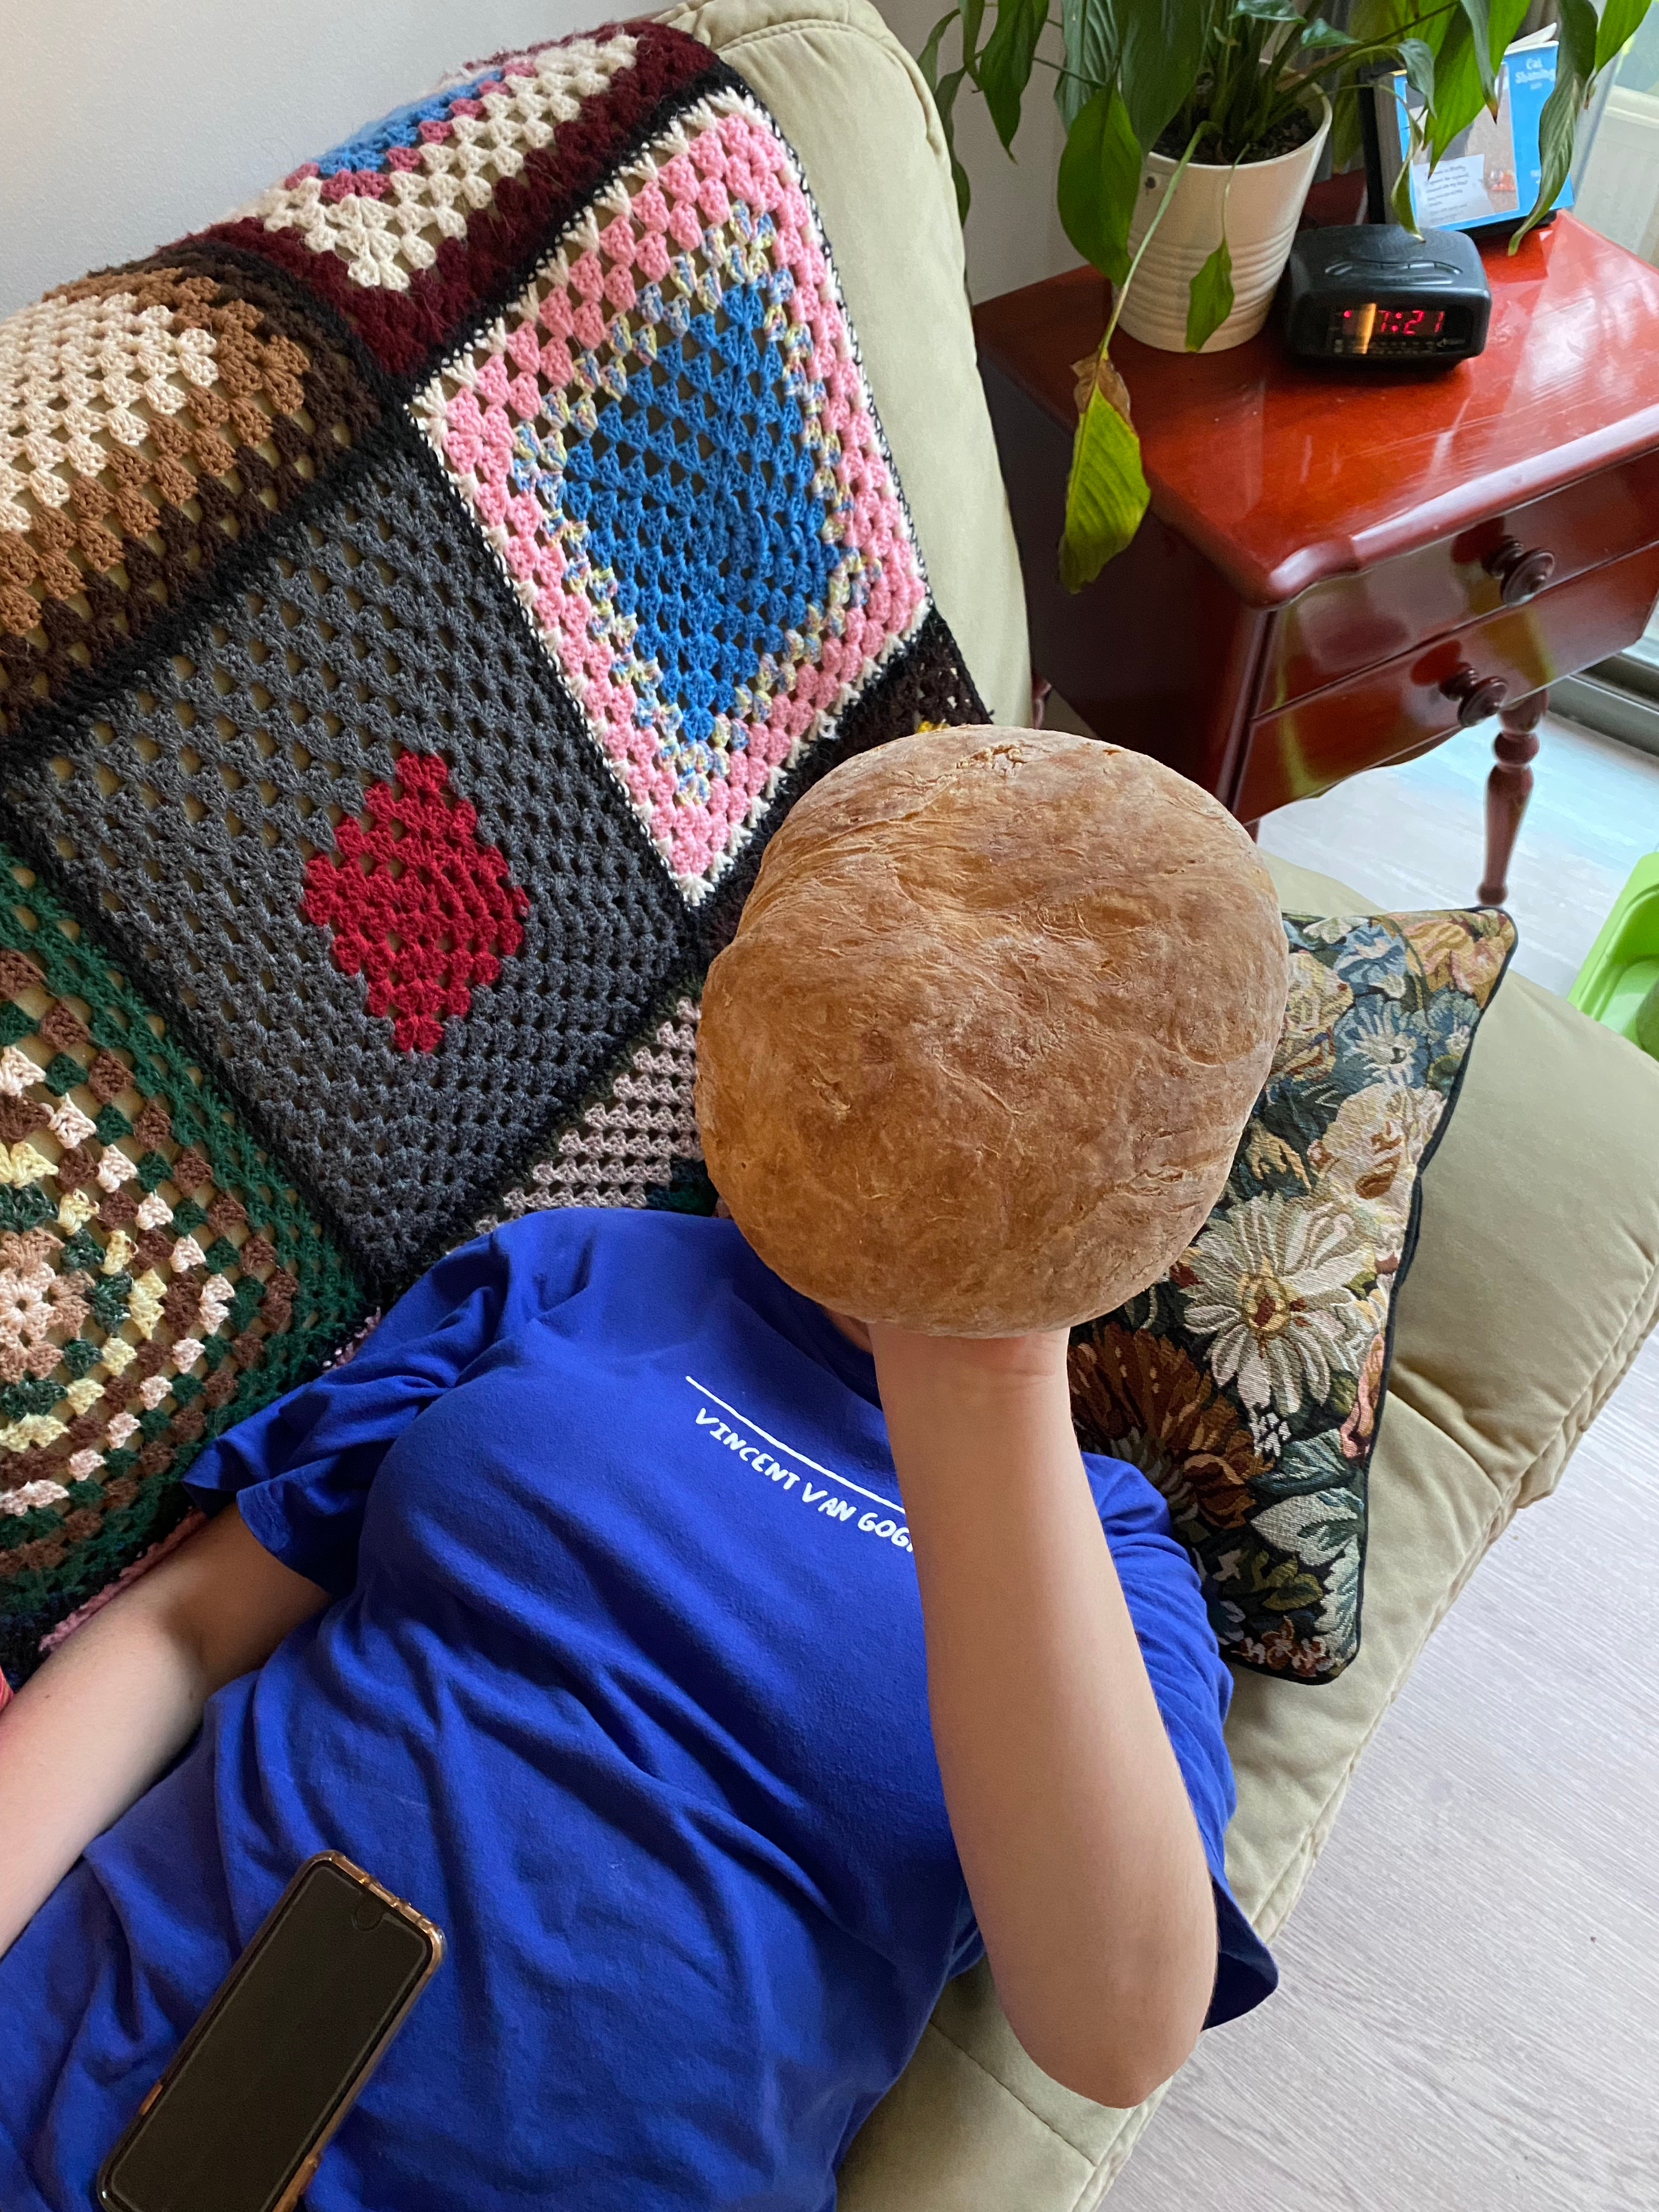
\includegraphics[keepaspectratio,width=\textwidth,height=\textheight]{Gallery/White bread (crusty, no-knead)}}\caption*{}\label{fig:White bread (crusty, no-knead)}\end{center}
\end{figure}
\newpage\begin{figure}[H]
\begin{center}\hyperref[rec:Almond Frangipane]{\includegraphics[keepaspectratio,width=\textheight,height=\textwidth,angle=-90]{Gallery/Almond Frangipane}}\caption*{}\label{fig:Almond Frangipane}\end{center}
\end{figure}
\newpage\begin{figure}[H]
\begin{center}\hyperref[rec:Choc Chip Biscuits]{\includegraphics[keepaspectratio,width=\textheight,height=\textwidth,angle=-90]{Gallery/Choc Chip Biscuits}}\caption*{}\label{fig:Choc Chip Biscuits}\end{center}
\end{figure}
\newpage\begin{figure}[H]
\begin{center}\hyperref[rec:Gingerbread Biscuits]{\includegraphics[keepaspectratio,width=\textheight,height=\textwidth,angle=-90]{Gallery/Gingerbread Biscuits}}\caption*{}\label{fig:Gingerbread Biscuits}\end{center}
\end{figure}
\newpage\begin{figure}[H]
\begin{center}\hyperref[rec:Vanilla Butter Cake]{\includegraphics[keepaspectratio,width=\textheight,height=\textwidth,angle=-90]{Gallery/Vanilla Butter Cake}}\caption*{}\label{fig:Vanilla Butter Cake}\end{center}
\end{figure}
\newpage\begin{figure}[H]
\begin{center}\hyperref[rec:Apple Crumble]{\includegraphics[keepaspectratio,width=\textheight,height=\textwidth,angle=-90]{Gallery/Apple Crumble}}\caption*{}\label{fig:Apple Crumble}\end{center}
\end{figure}
\newpage\begin{figure}[H]
\begin{center}\hyperref[rec:Banana Split]{\includegraphics[keepaspectratio,width=\textheight,height=\textwidth,angle=-90]{Gallery/Banana Split}}\caption*{}\label{fig:Banana Split}\end{center}
\end{figure}
\newpage\begin{figure}[H]
\begin{center}\hyperref[rec:Apple Cinnamon Muffins]{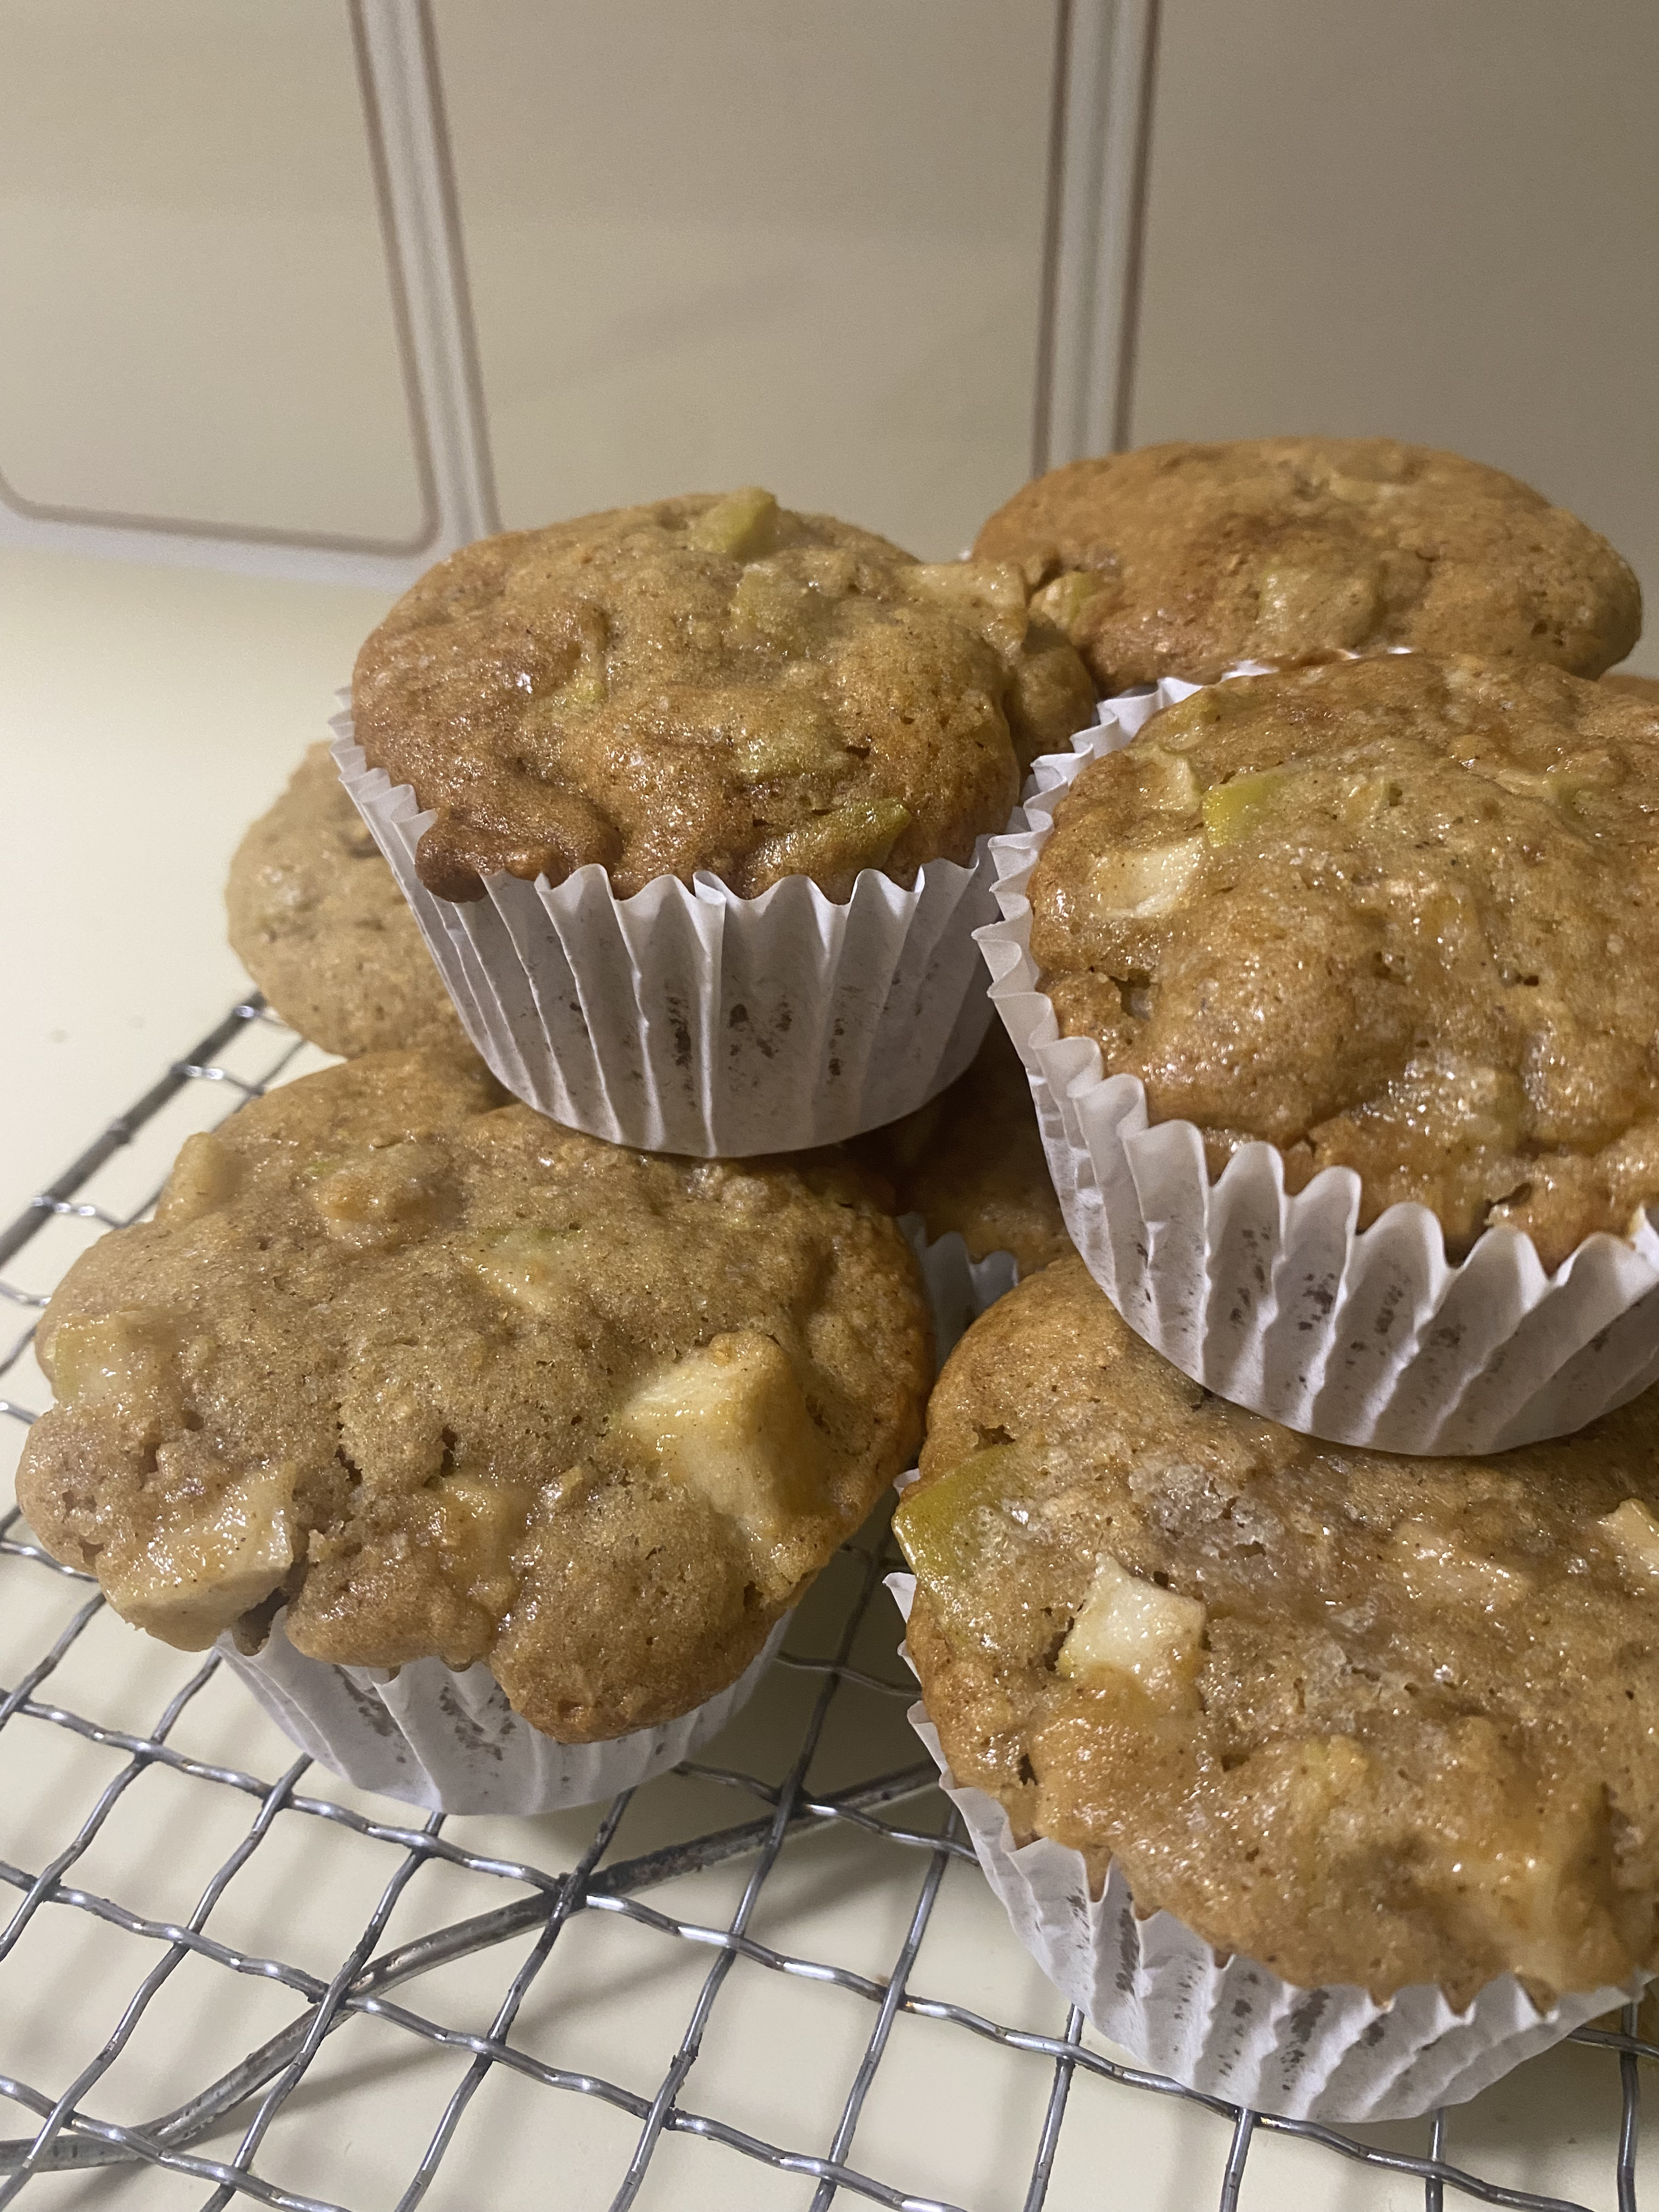
\includegraphics[keepaspectratio,width=\textwidth,height=\textheight]{Gallery/Apple Cinnamon Muffins}}\caption*{}\label{fig:Apple Cinnamon Muffins}\end{center}
\end{figure}
\newpage\begin{figure}[H]
\begin{center}\hyperref[rec:Strawberry Flan]{\includegraphics[keepaspectratio,width=\textheight,height=\textwidth,angle=-90]{Gallery/Strawberry Flan}}\caption*{}\label{fig:Strawberry Flan}\end{center}
\end{figure}
\newpage\begin{figure}[H]
\begin{center}\hyperref[rec:Enchiladas]{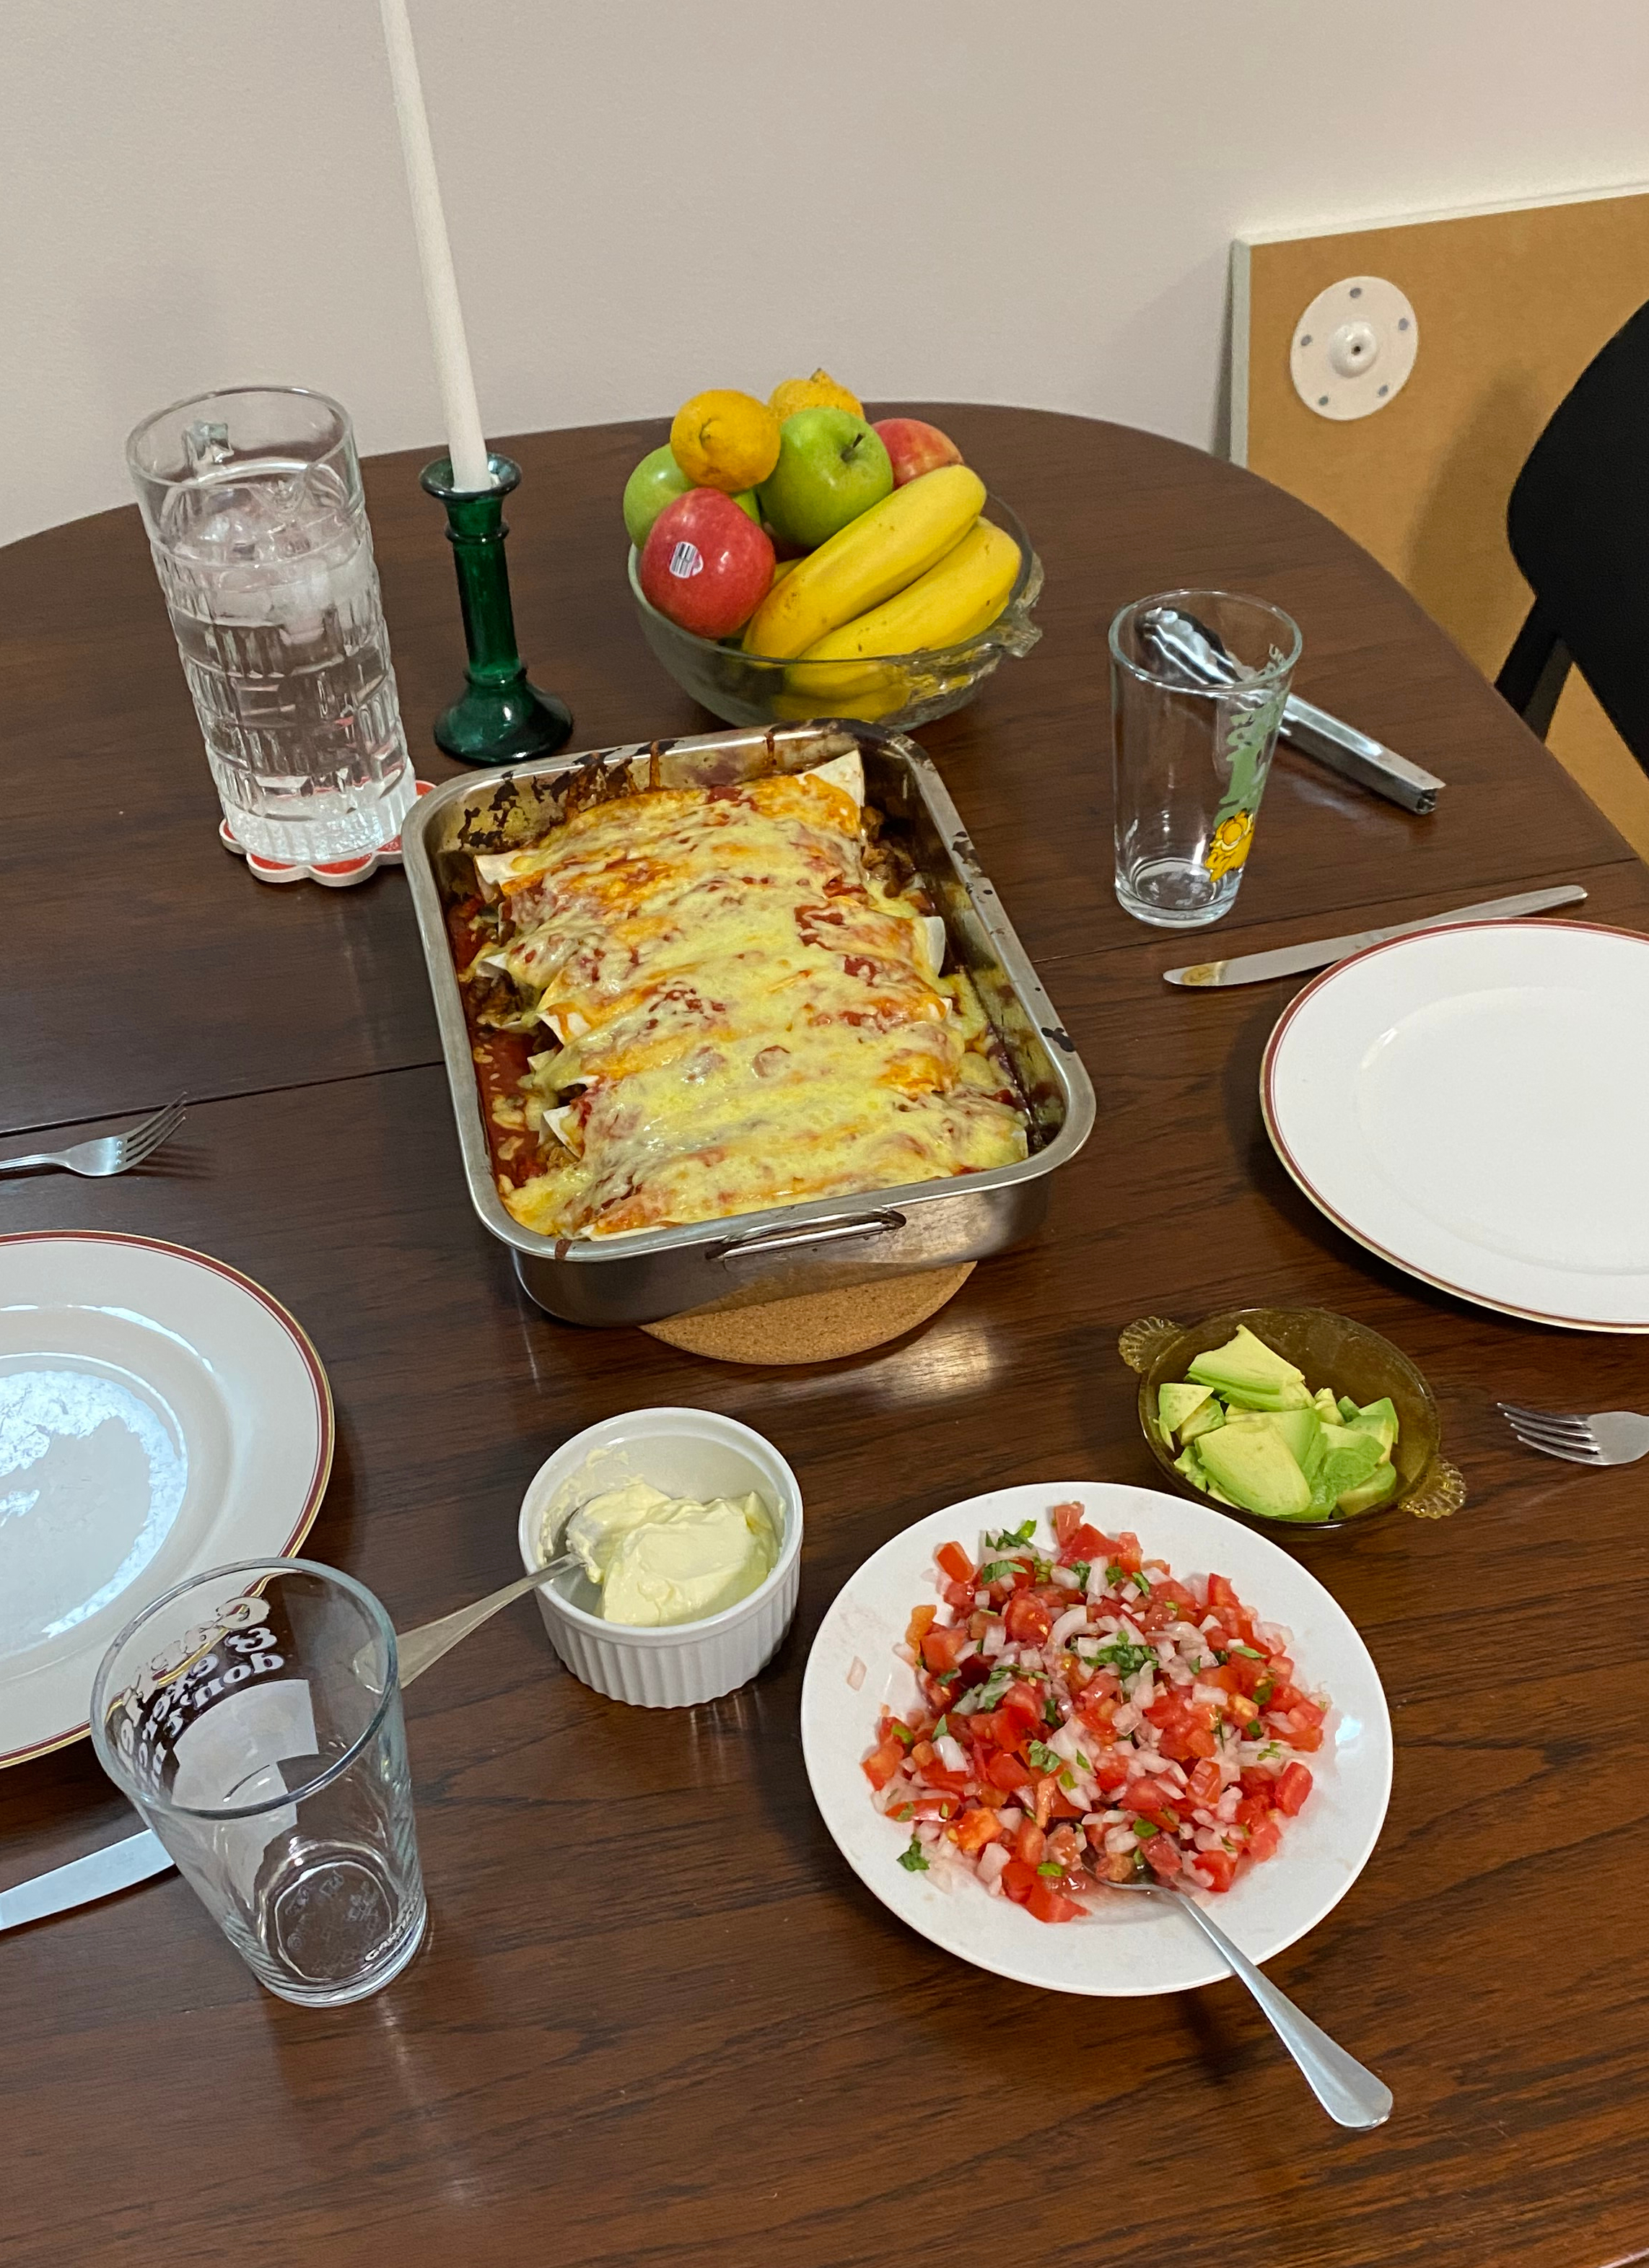
\includegraphics[keepaspectratio,width=\textwidth,height=\textheight]{Gallery/Enchiladas}}\caption*{}\label{fig:Enchiladas}\end{center}
\end{figure}
\newpage\begin{figure}[H]
\begin{center}\hyperref[rec:Lasagne]{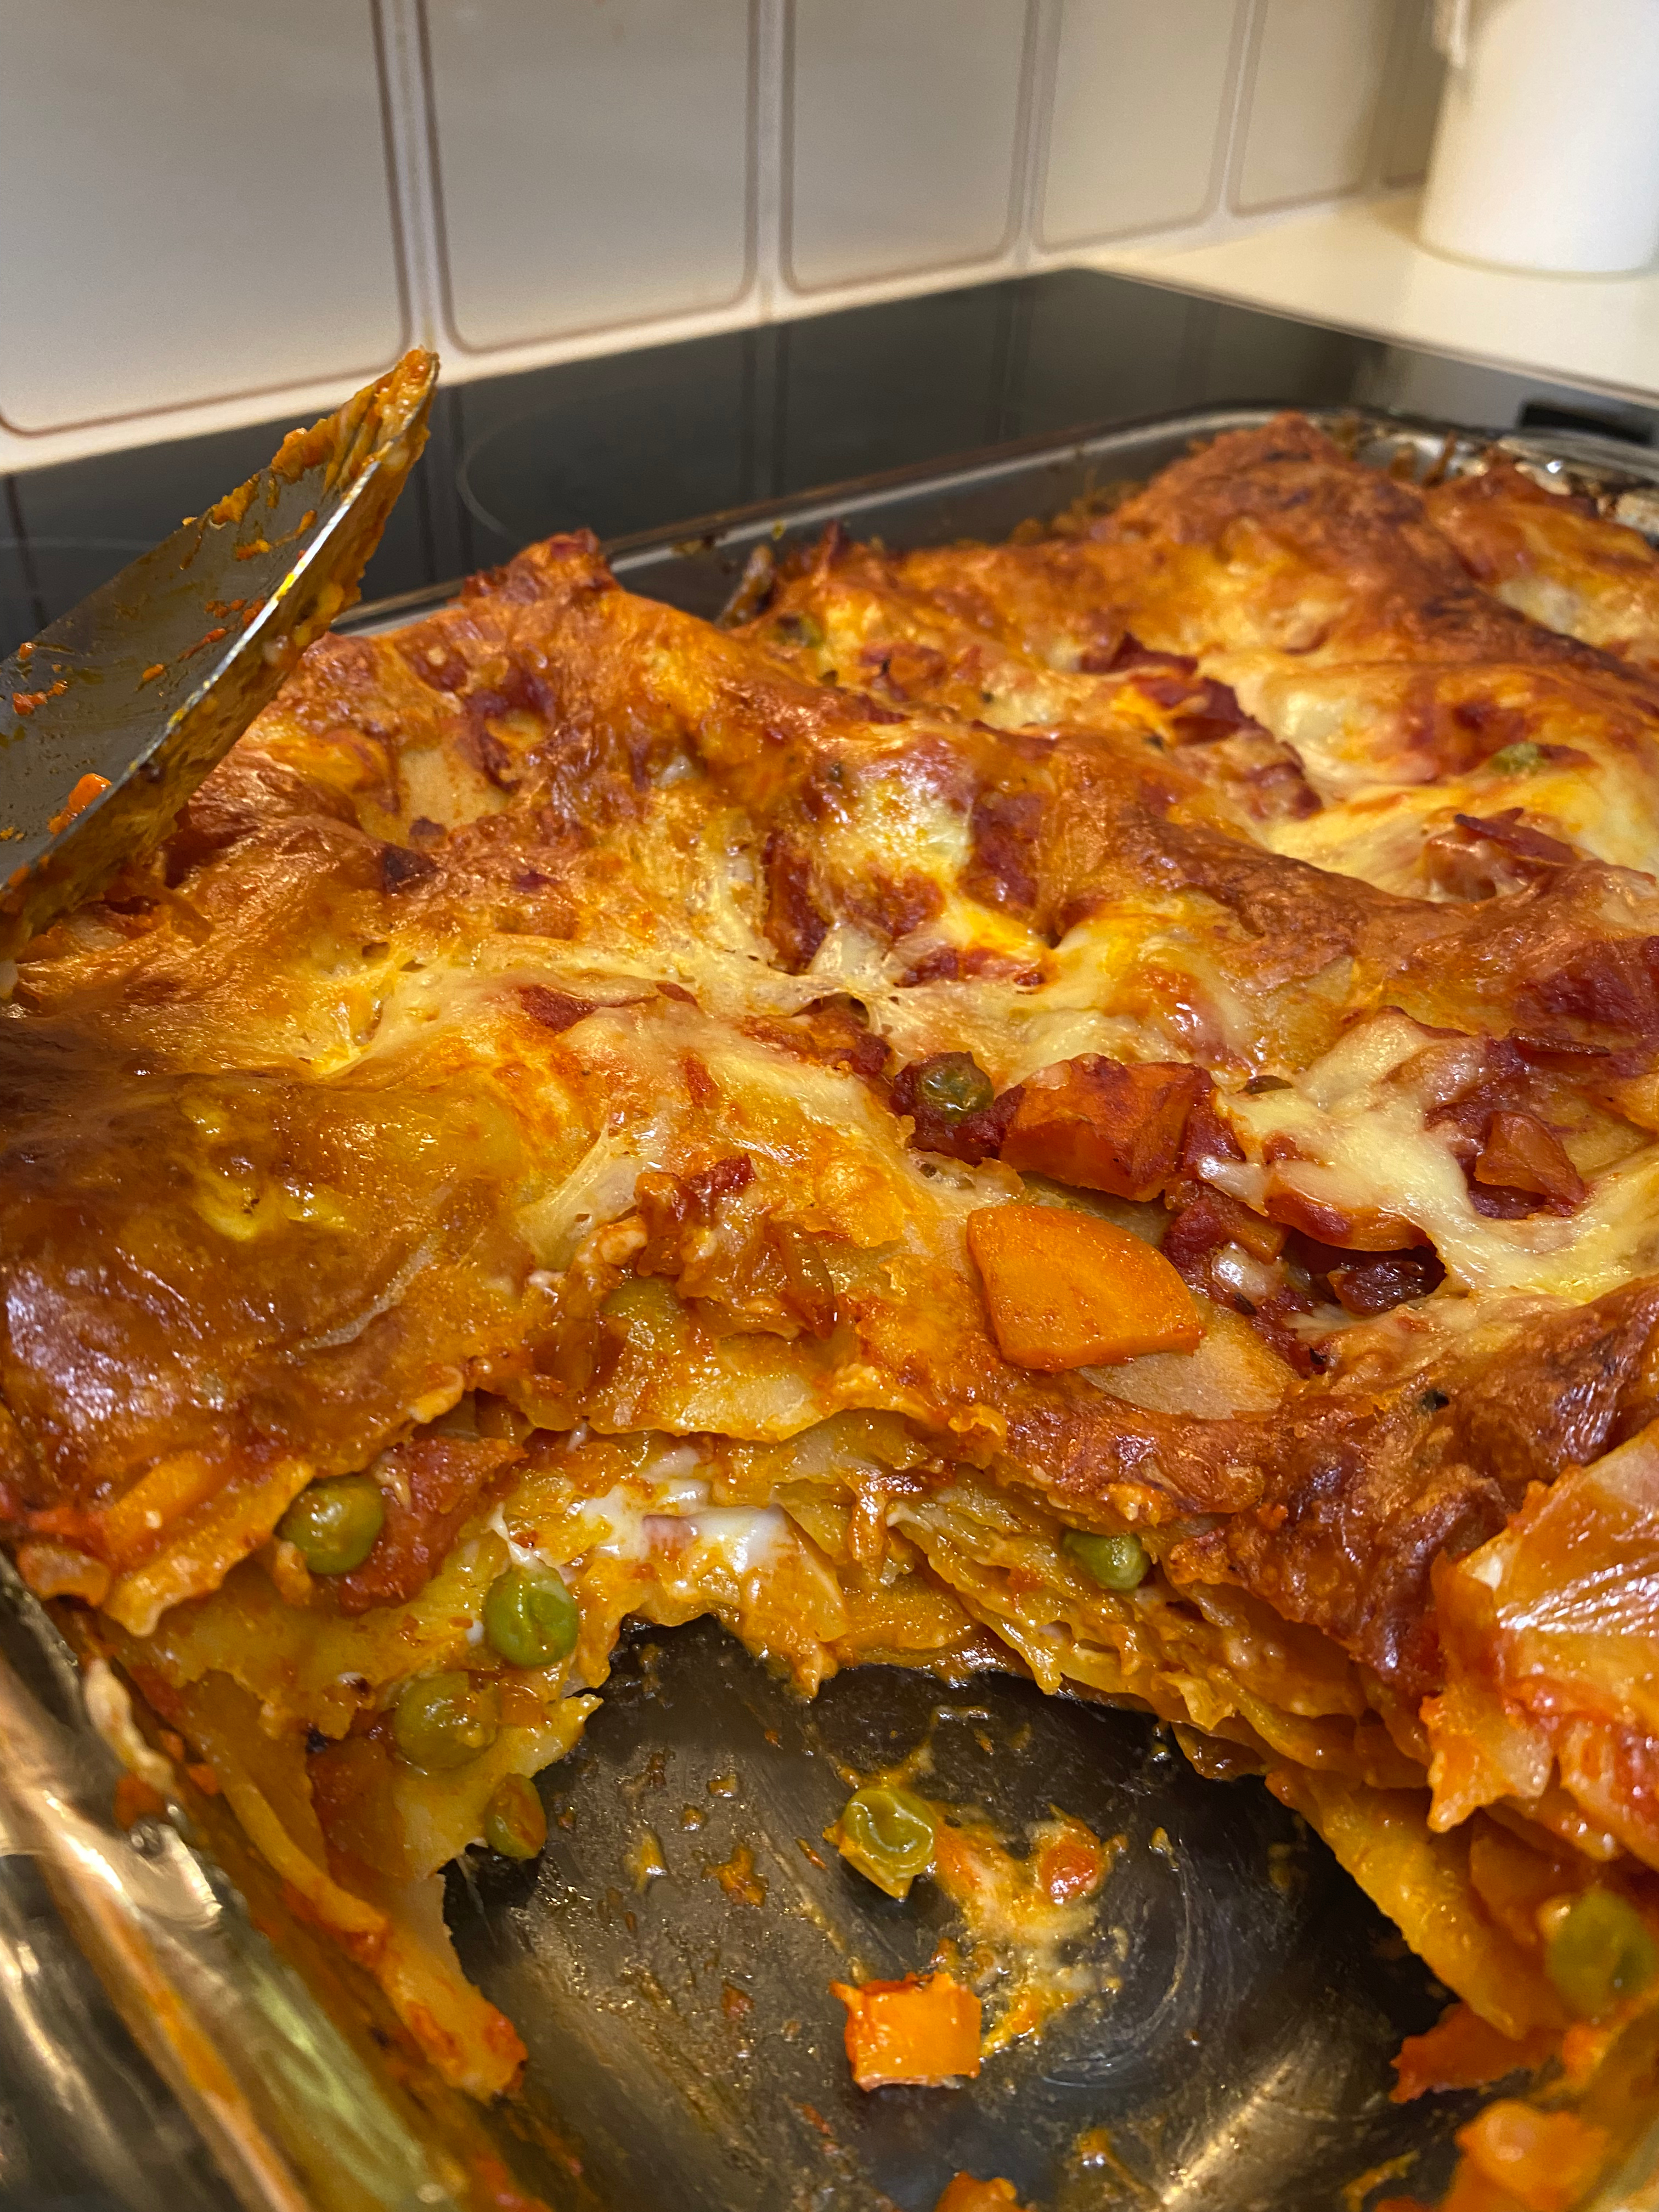
\includegraphics[keepaspectratio,width=\textwidth,height=\textheight]{Gallery/Lasagne}}\caption*{}\label{fig:Lasagne}\end{center}
\end{figure}
\newpage\begin{figure}[H]
\begin{center}\hyperref[rec:Nachos]{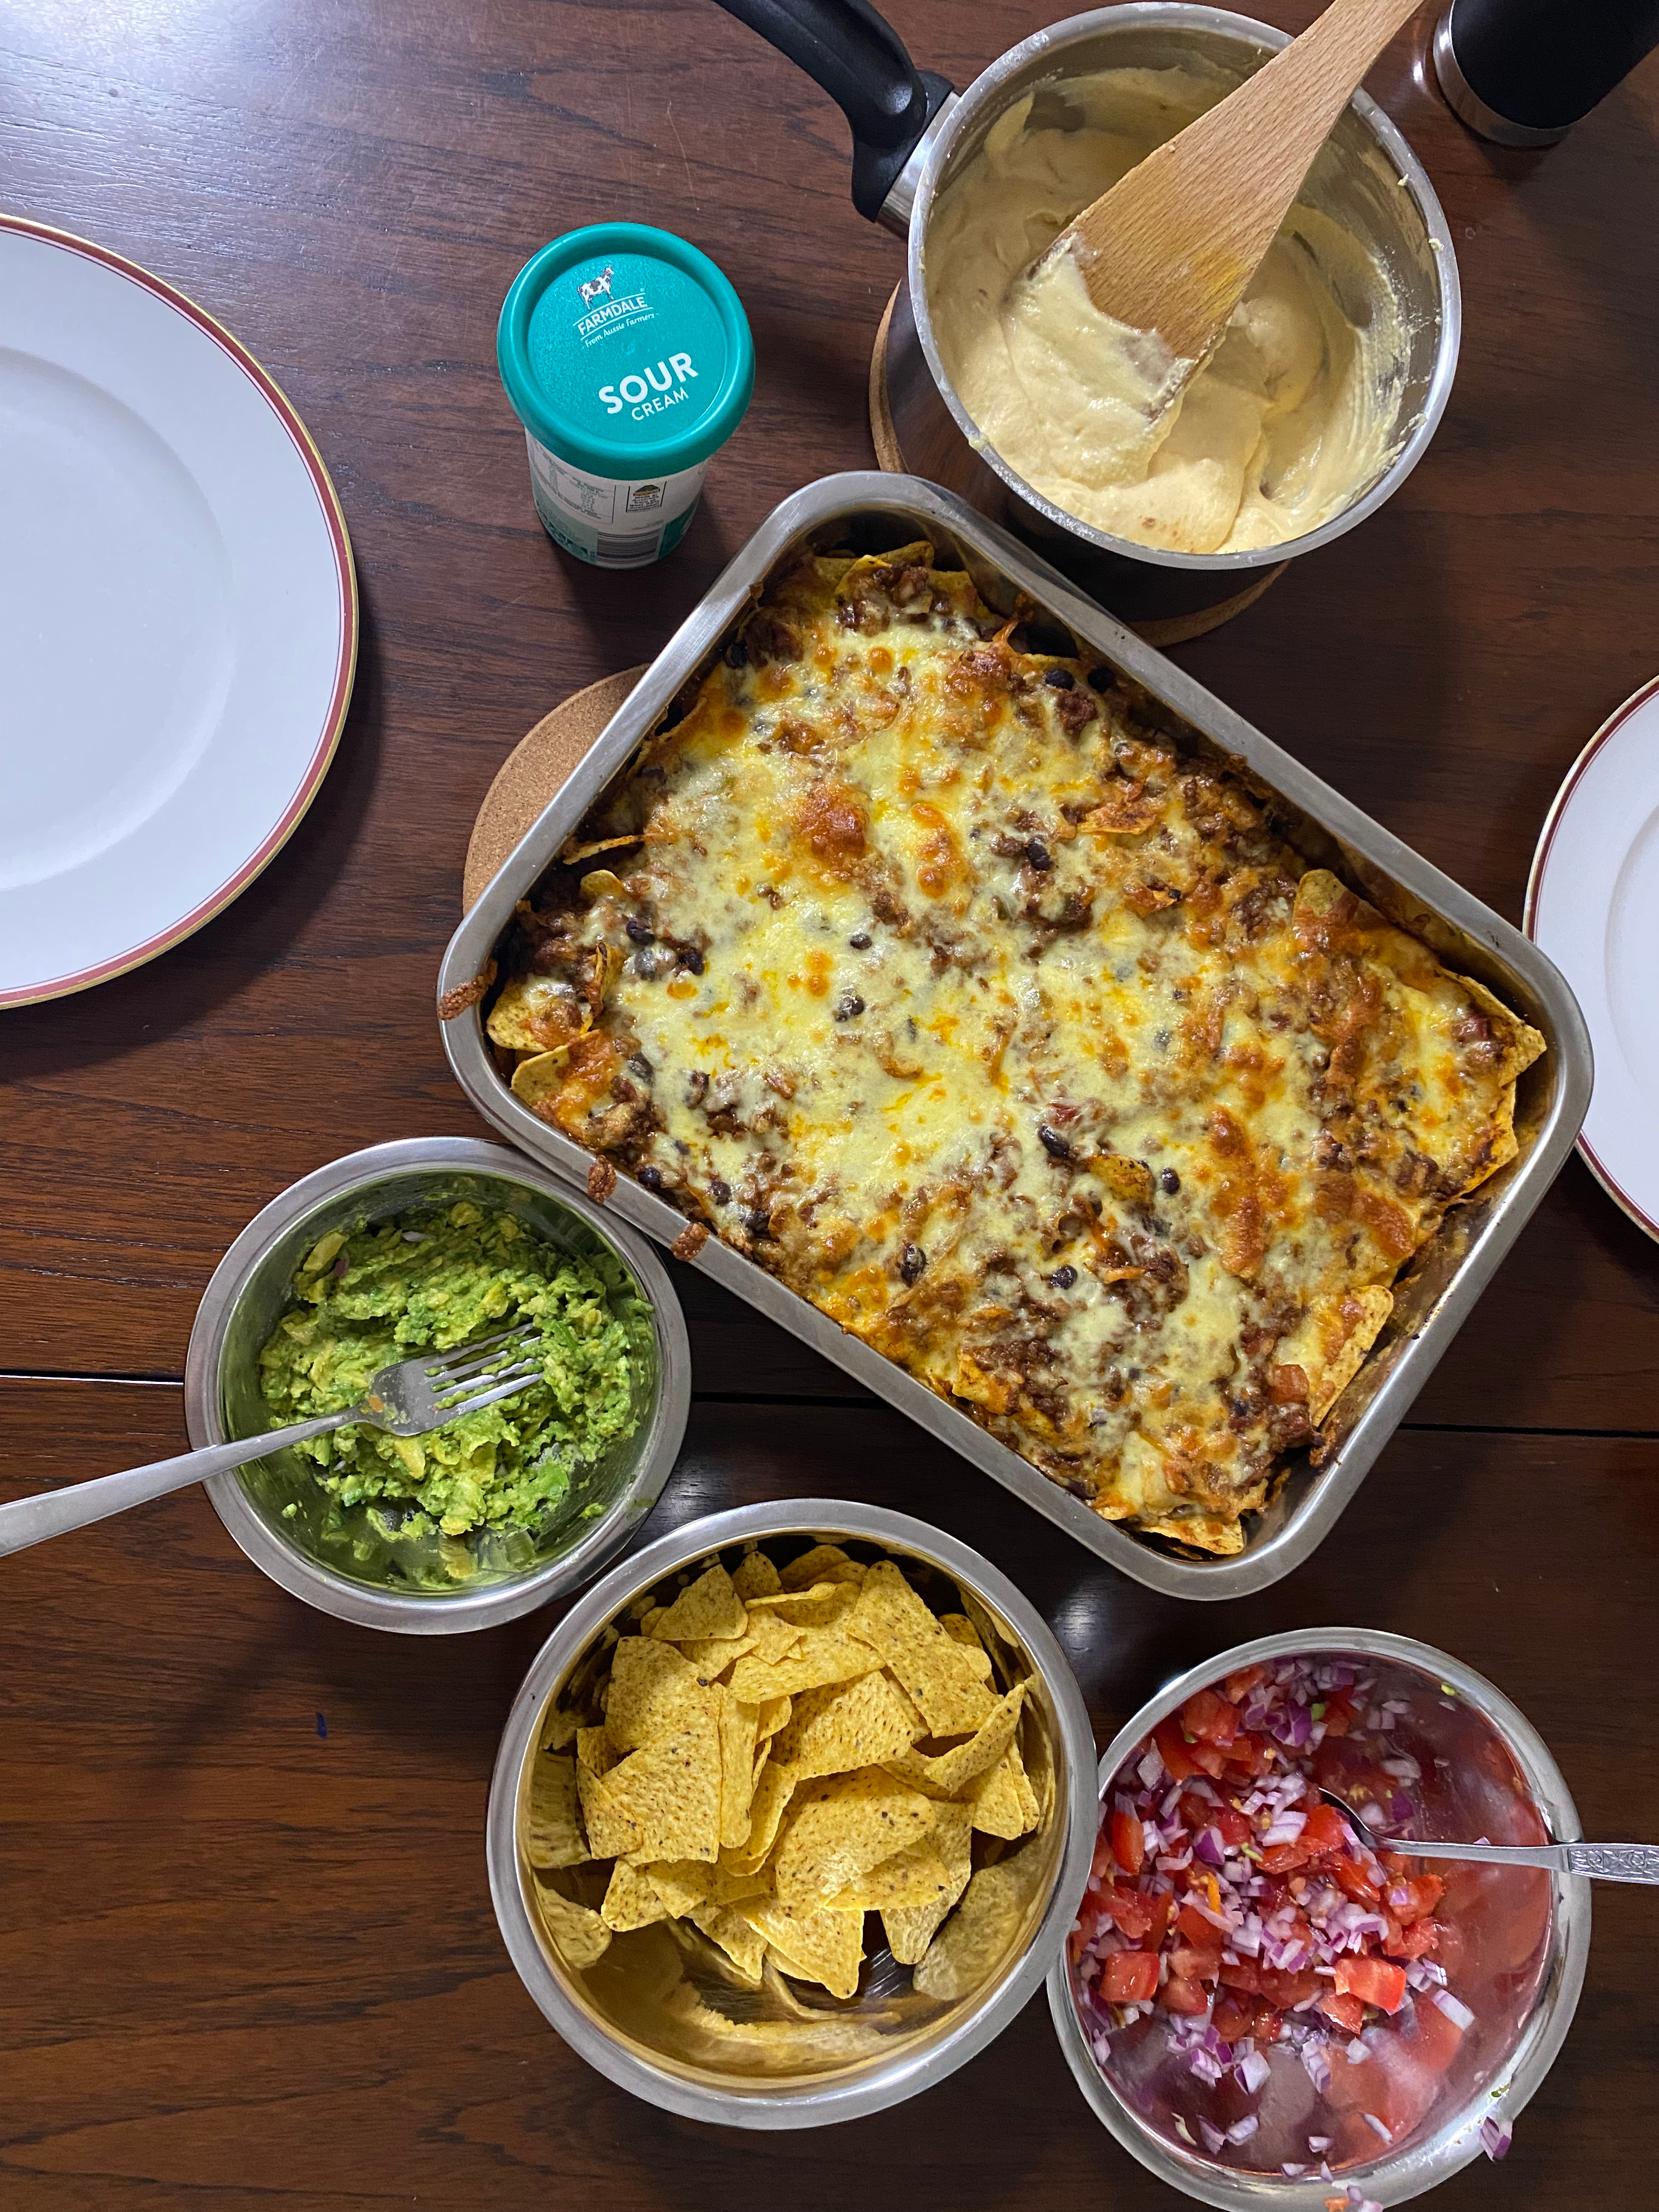
\includegraphics[keepaspectratio,width=\textwidth,height=\textheight]{Gallery/Nachos}}\caption*{}\label{fig:Nachos}\end{center}
\end{figure}
\newpage\begin{figure}[H]
\begin{center}\hyperref[rec:Tuna Pasta Bake]{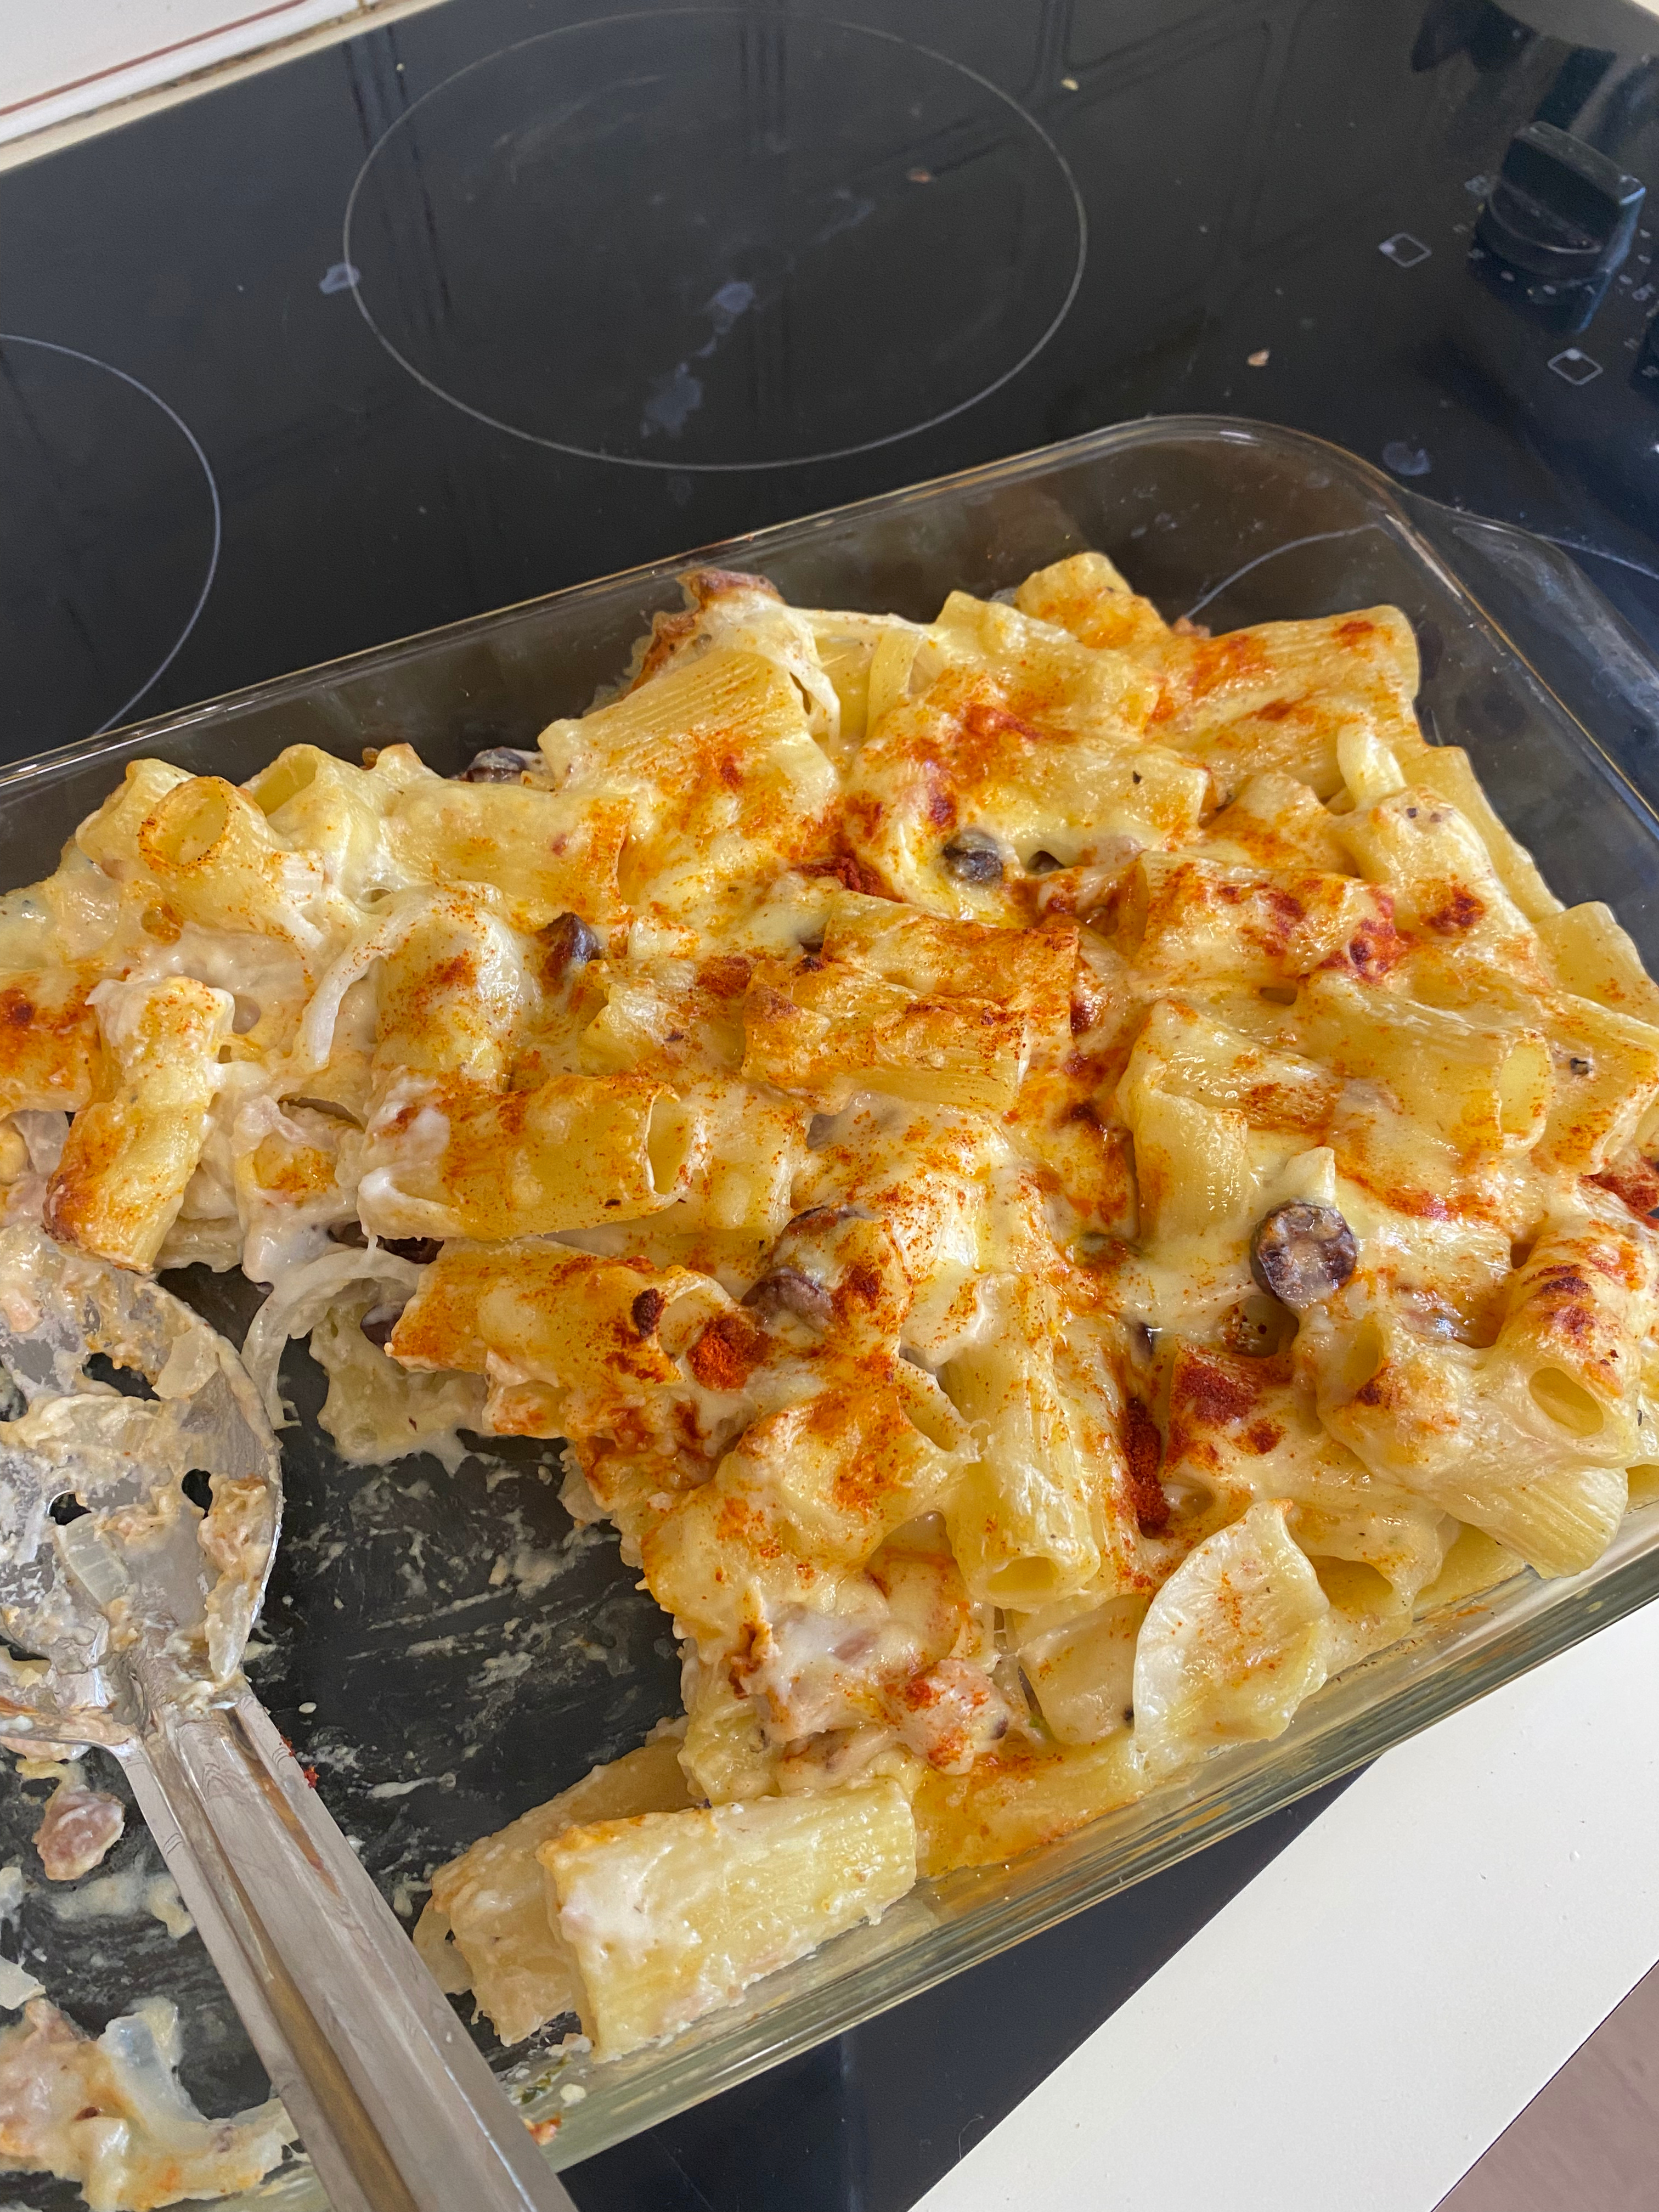
\includegraphics[keepaspectratio,width=\textwidth,height=\textheight]{Gallery/Tuna Pasta Bake}}\caption*{}\label{fig:Tuna Pasta Bake}\end{center}
\end{figure}
\newpage\begin{figure}[H]
\begin{center}\hyperref[rec:Sausage sizzle]{\includegraphics[keepaspectratio,width=\textwidth,height=\textheight]{Gallery/Sausage sizzle}}\caption*{}\label{fig:Sausage sizzle}\end{center}
\end{figure}
\newpage\begin{figure}[H]
\begin{center}\hyperref[rec:Beef Burgers]{\includegraphics[keepaspectratio,width=\textheight,height=\textwidth,angle=-90]{Gallery/Beef Burgers}}\caption*{}\label{fig:Beef Burgers}\end{center}
\end{figure}
\newpage\begin{figure}[H]
\begin{center}\hyperref[rec:Chickpea Curry]{\includegraphics[keepaspectratio,width=\textheight,height=\textwidth,angle=-90]{Gallery/Chickpea Curry}}\caption*{}\label{fig:Chickpea Curry}\end{center}
\end{figure}
\newpage\begin{figure}[H]
\begin{center}\hyperref[rec:Potato Curry]{\includegraphics[keepaspectratio,width=\textheight,height=\textwidth,angle=-90]{Gallery/Potato Curry}}\caption*{}\label{fig:Potato Curry}\end{center}
\end{figure}
\newpage\begin{figure}[H]
\begin{center}\hyperref[rec:Chicken Schnitzel]{\includegraphics[keepaspectratio,width=\textwidth,height=\textheight]{Gallery/Chicken Schnitzel}}\caption*{}\label{fig:Chicken Schnitzel}\end{center}
\end{figure}
\newpage\begin{figure}[H]
\begin{center}\hyperref[rec:Chicken Shawarma]{\includegraphics[keepaspectratio,width=\textheight,height=\textwidth,angle=-90]{Gallery/Chicken Shawarma}}\caption*{}\label{fig:Chicken Shawarma}\end{center}
\end{figure}
\newpage\begin{figure}[H]
\begin{center}\hyperref[rec:Gyros]{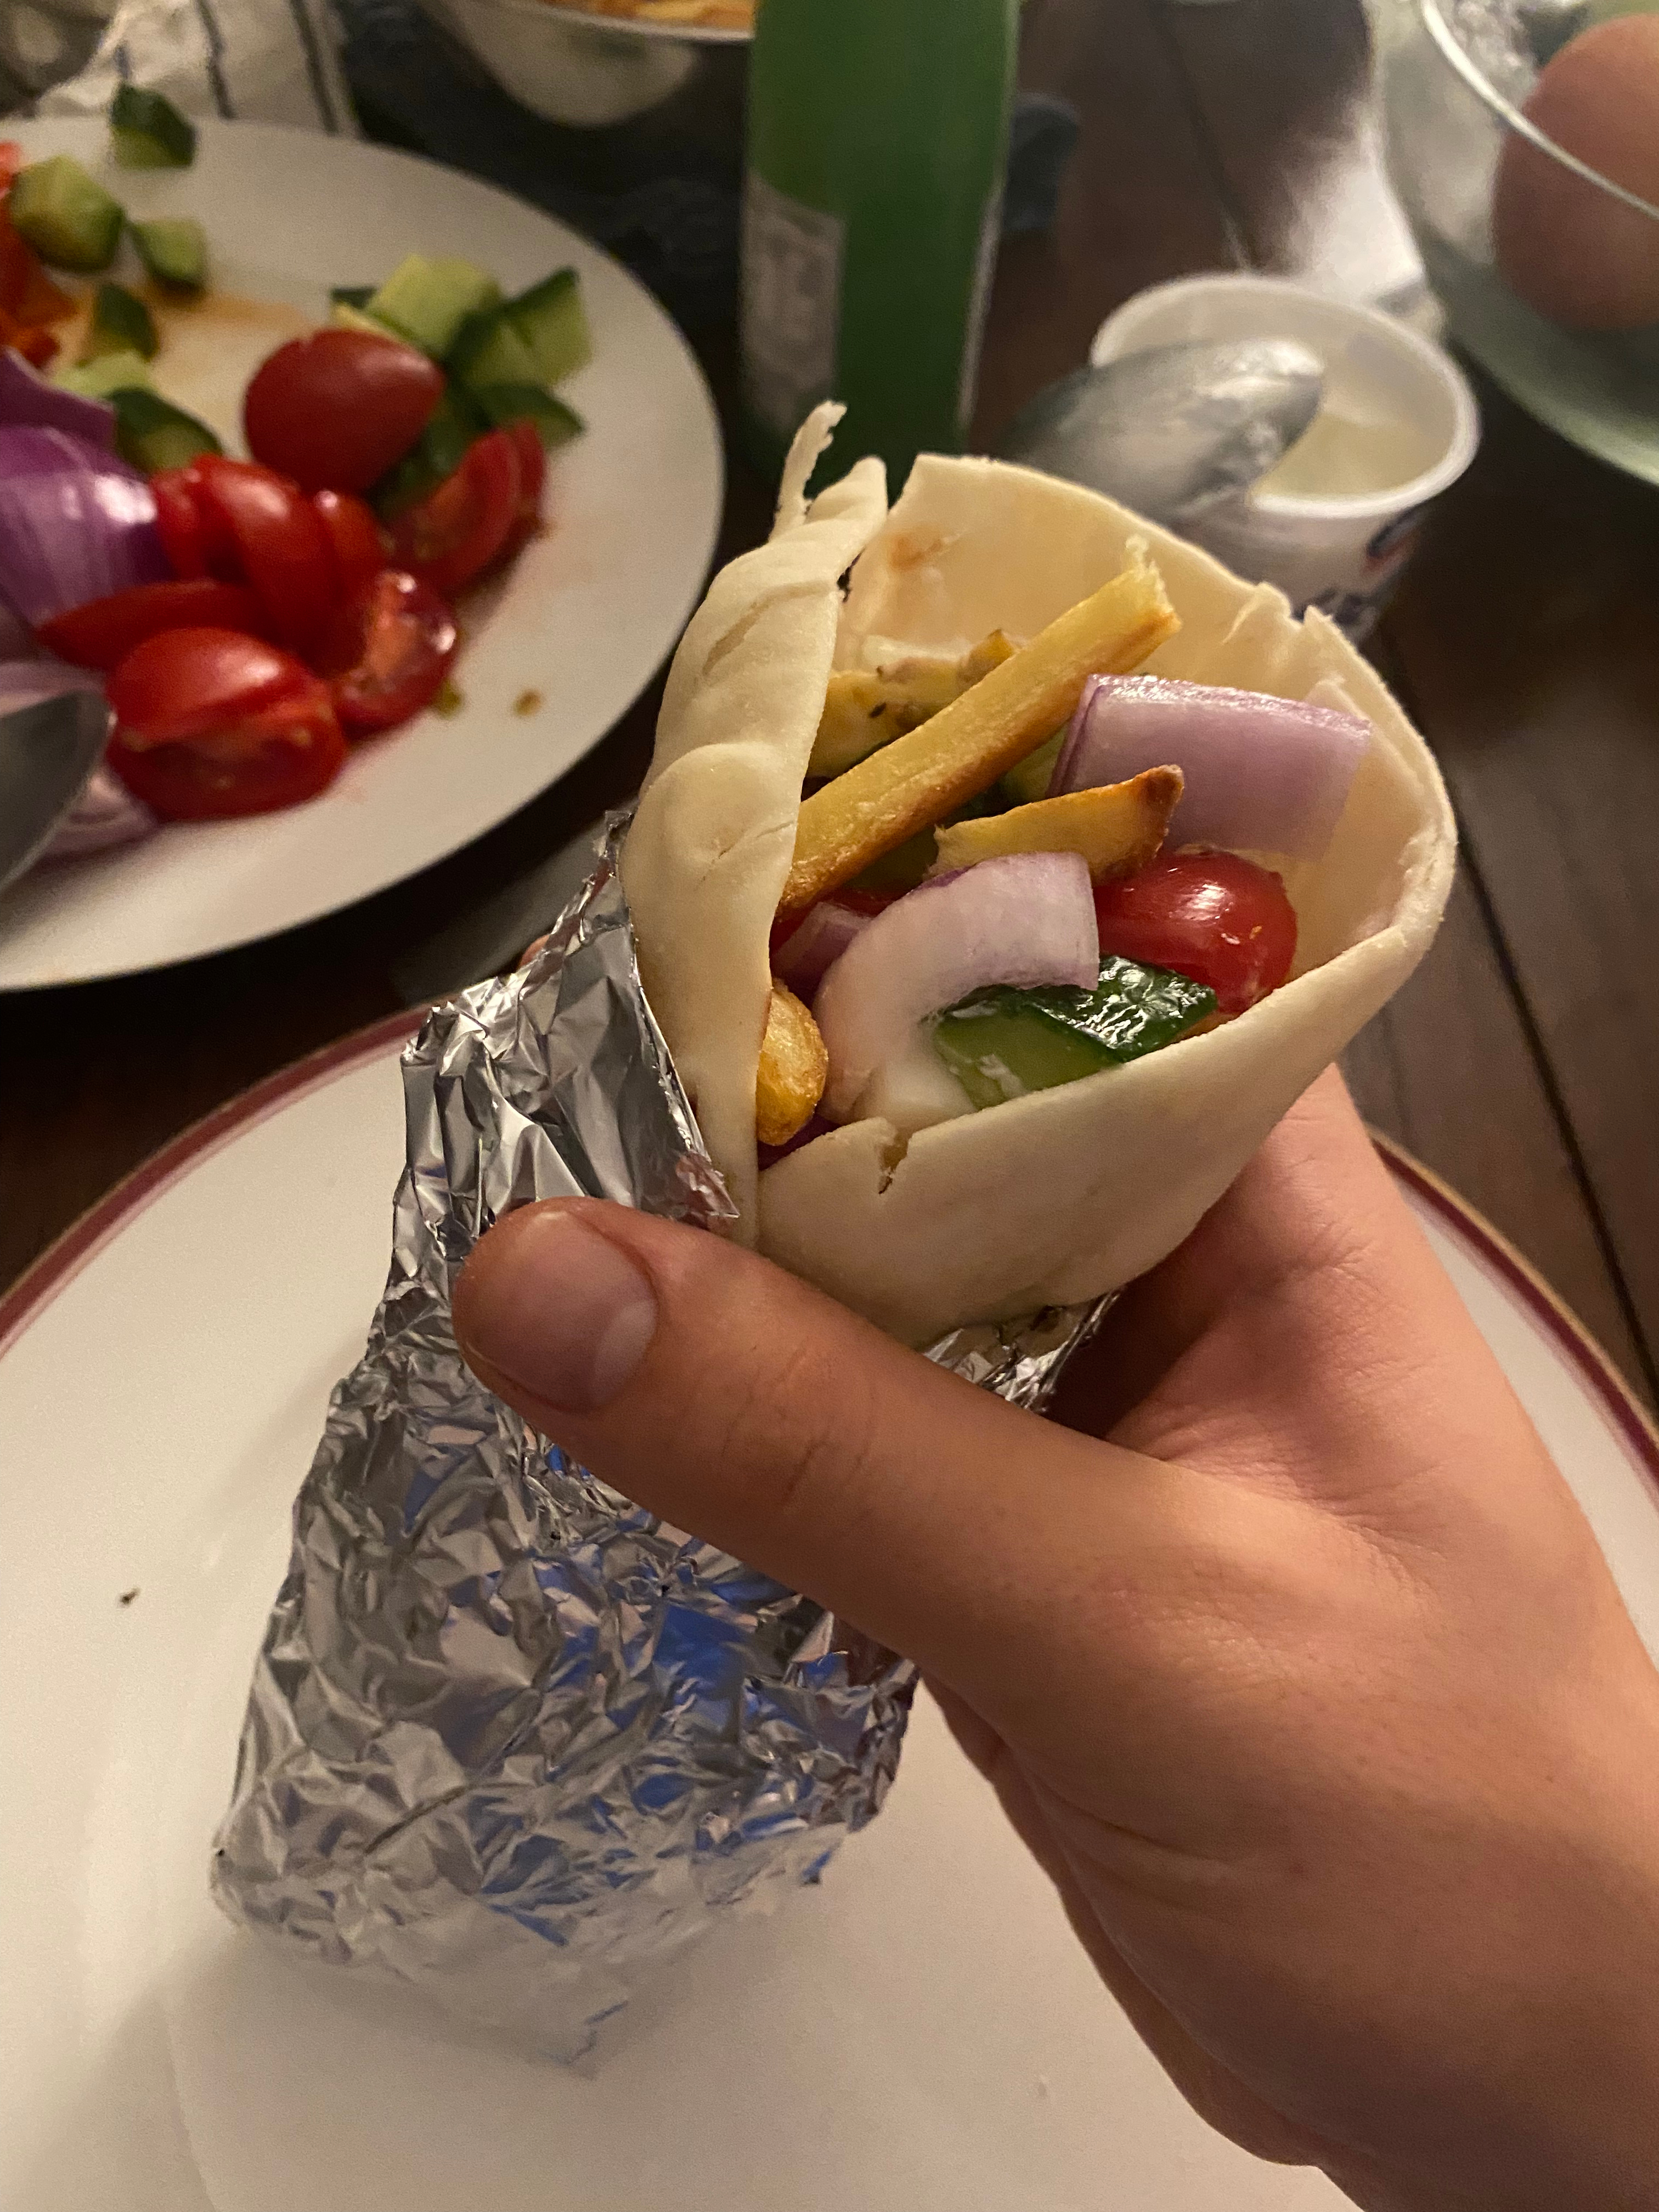
\includegraphics[keepaspectratio,width=\textwidth,height=\textheight]{Gallery/Gyros}}\caption*{}\label{fig:Gyros}\end{center}
\end{figure}
\newpage\begin{figure}[H]
\begin{center}\hyperref[rec:Chow Mein]{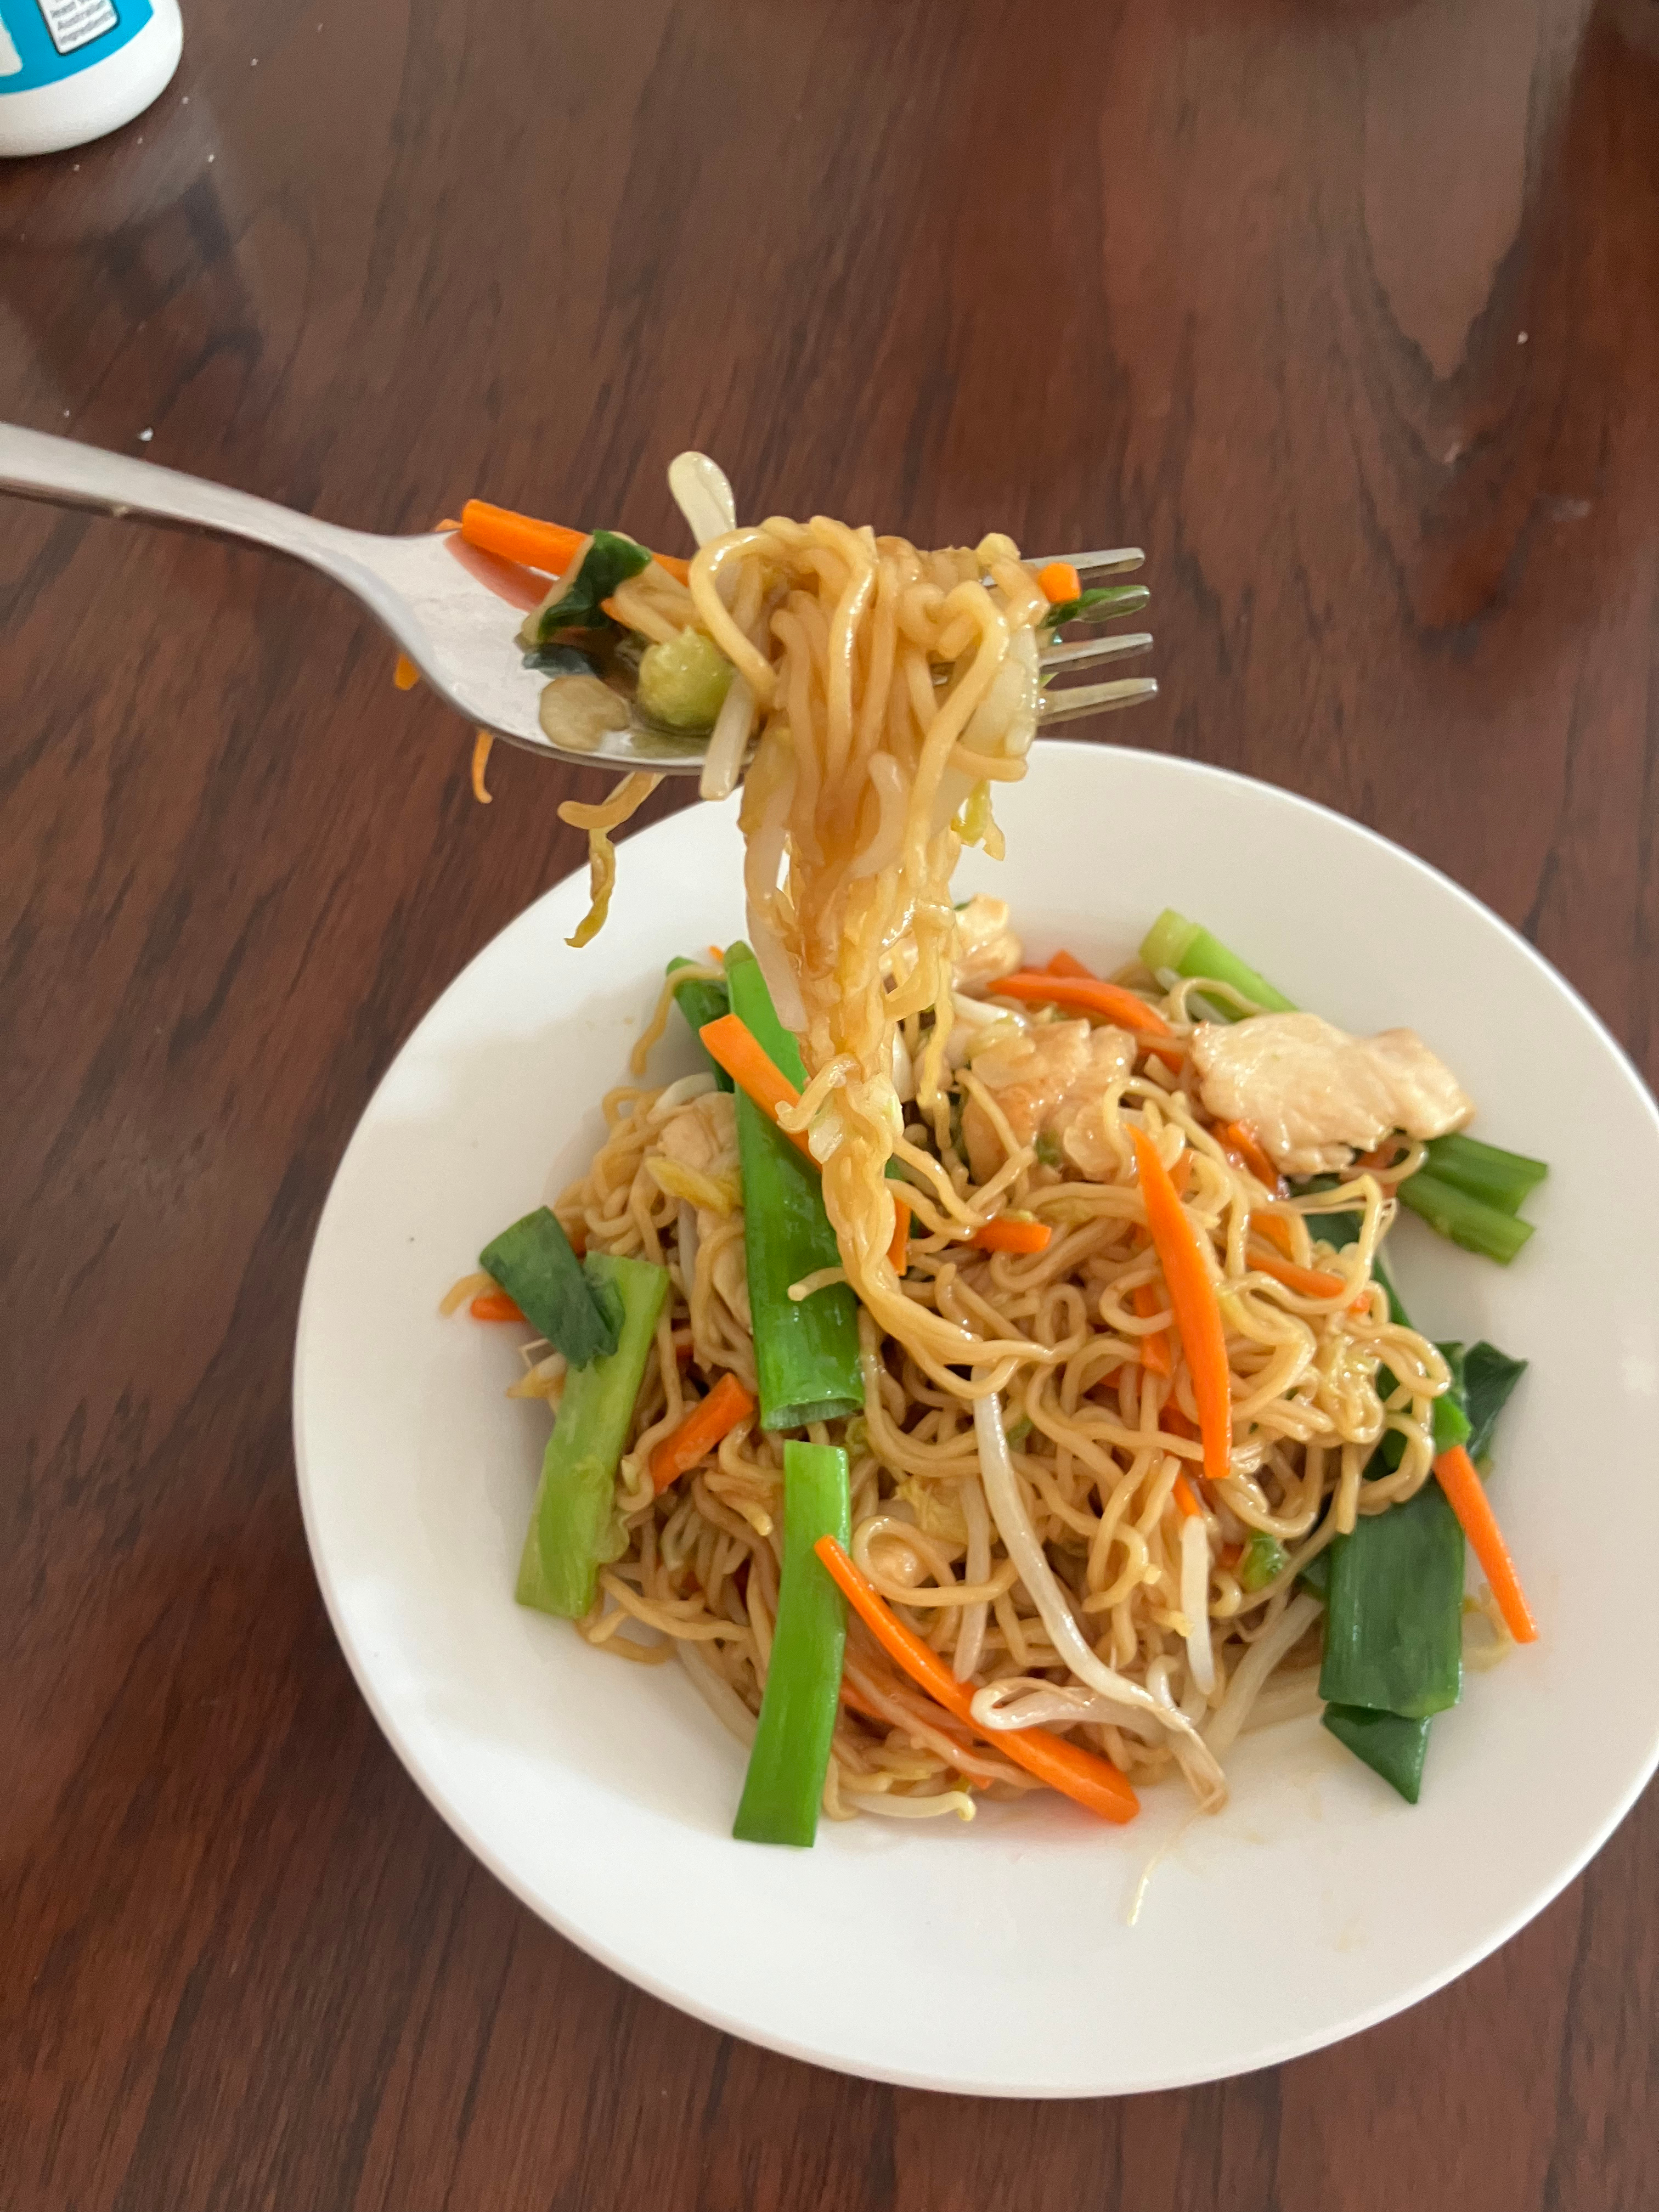
\includegraphics[keepaspectratio,width=\textwidth,height=\textheight]{Gallery/Chow Mein}}\caption*{}\label{fig:Chow Mein}\end{center}
\end{figure}
\newpage\begin{figure}[H]
\begin{center}\hyperref[rec:Hokkien Mee]{\includegraphics[keepaspectratio,width=\textwidth,height=\textheight]{Gallery/Hokkien Mee}}\caption*{}\label{fig:Hokkien Mee}\end{center}
\end{figure}
\newpage\begin{figure}[H]
\begin{center}\hyperref[rec:Pad See Ew]{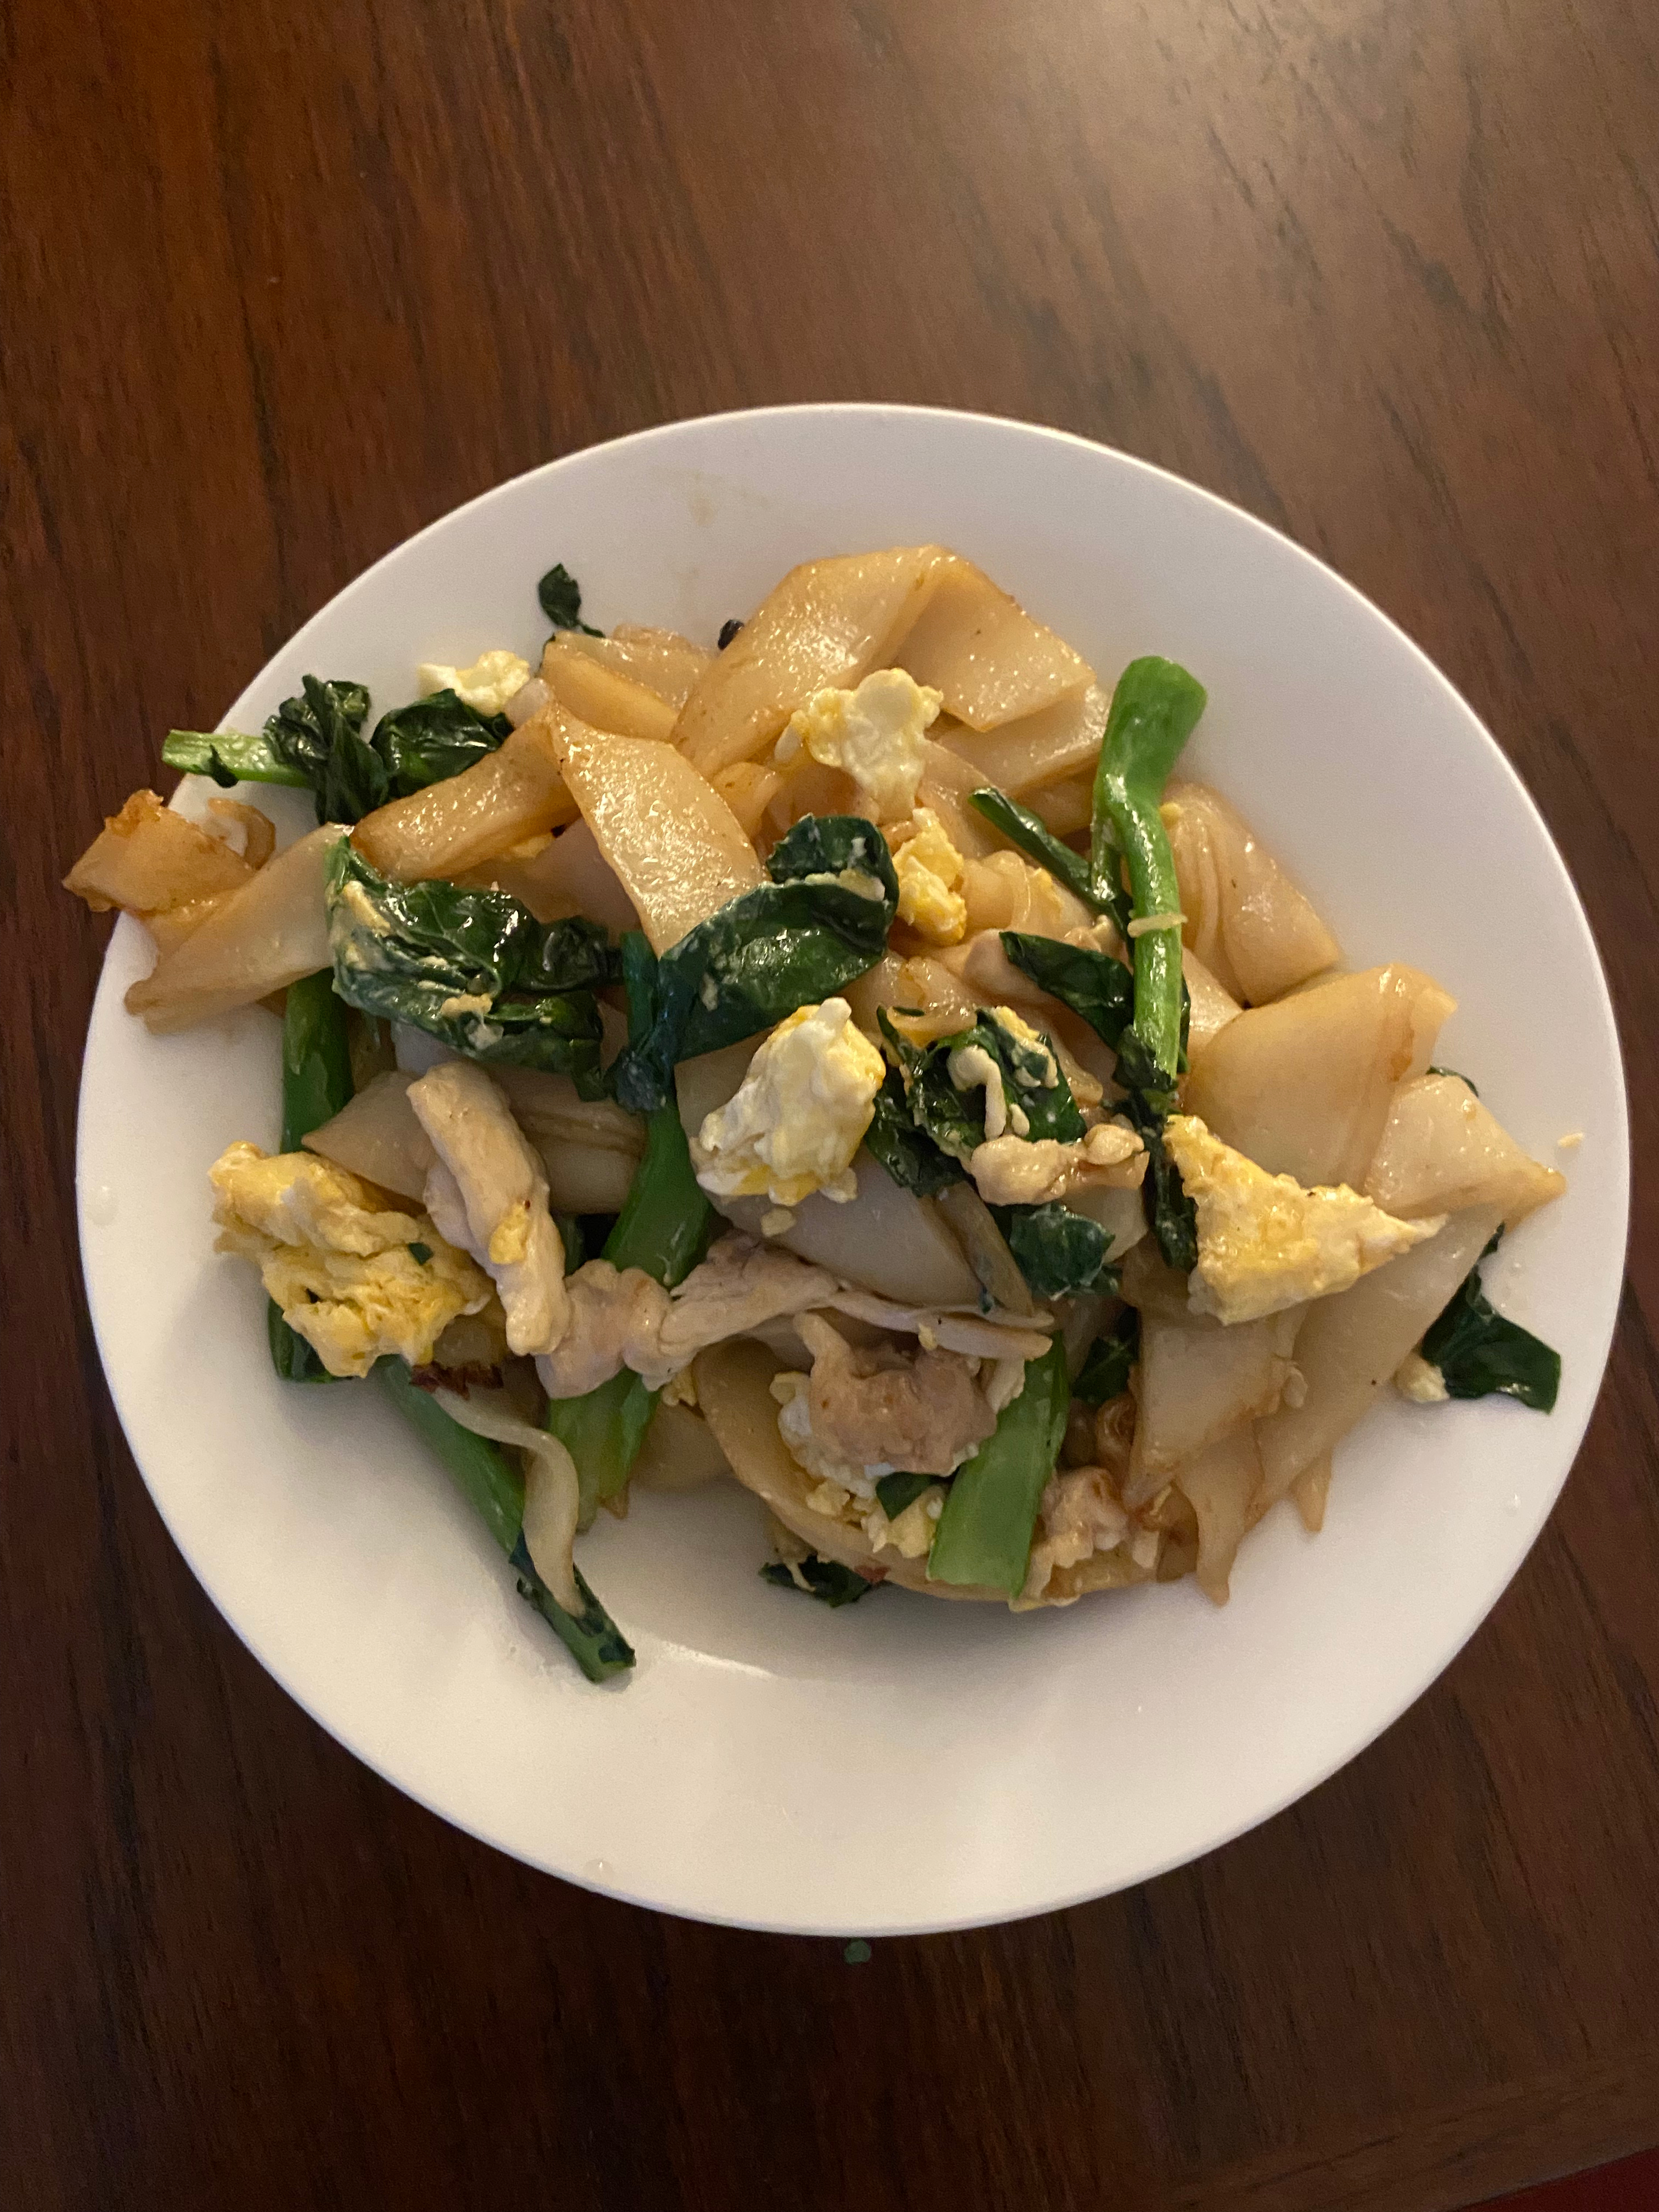
\includegraphics[keepaspectratio,width=\textwidth,height=\textheight]{Gallery/Pad See Ew}}\caption*{}\label{fig:Pad See Ew}\end{center}
\end{figure}
\newpage\begin{figure}[H]
\begin{center}\hyperref[rec:Basil Chicken Pesto]{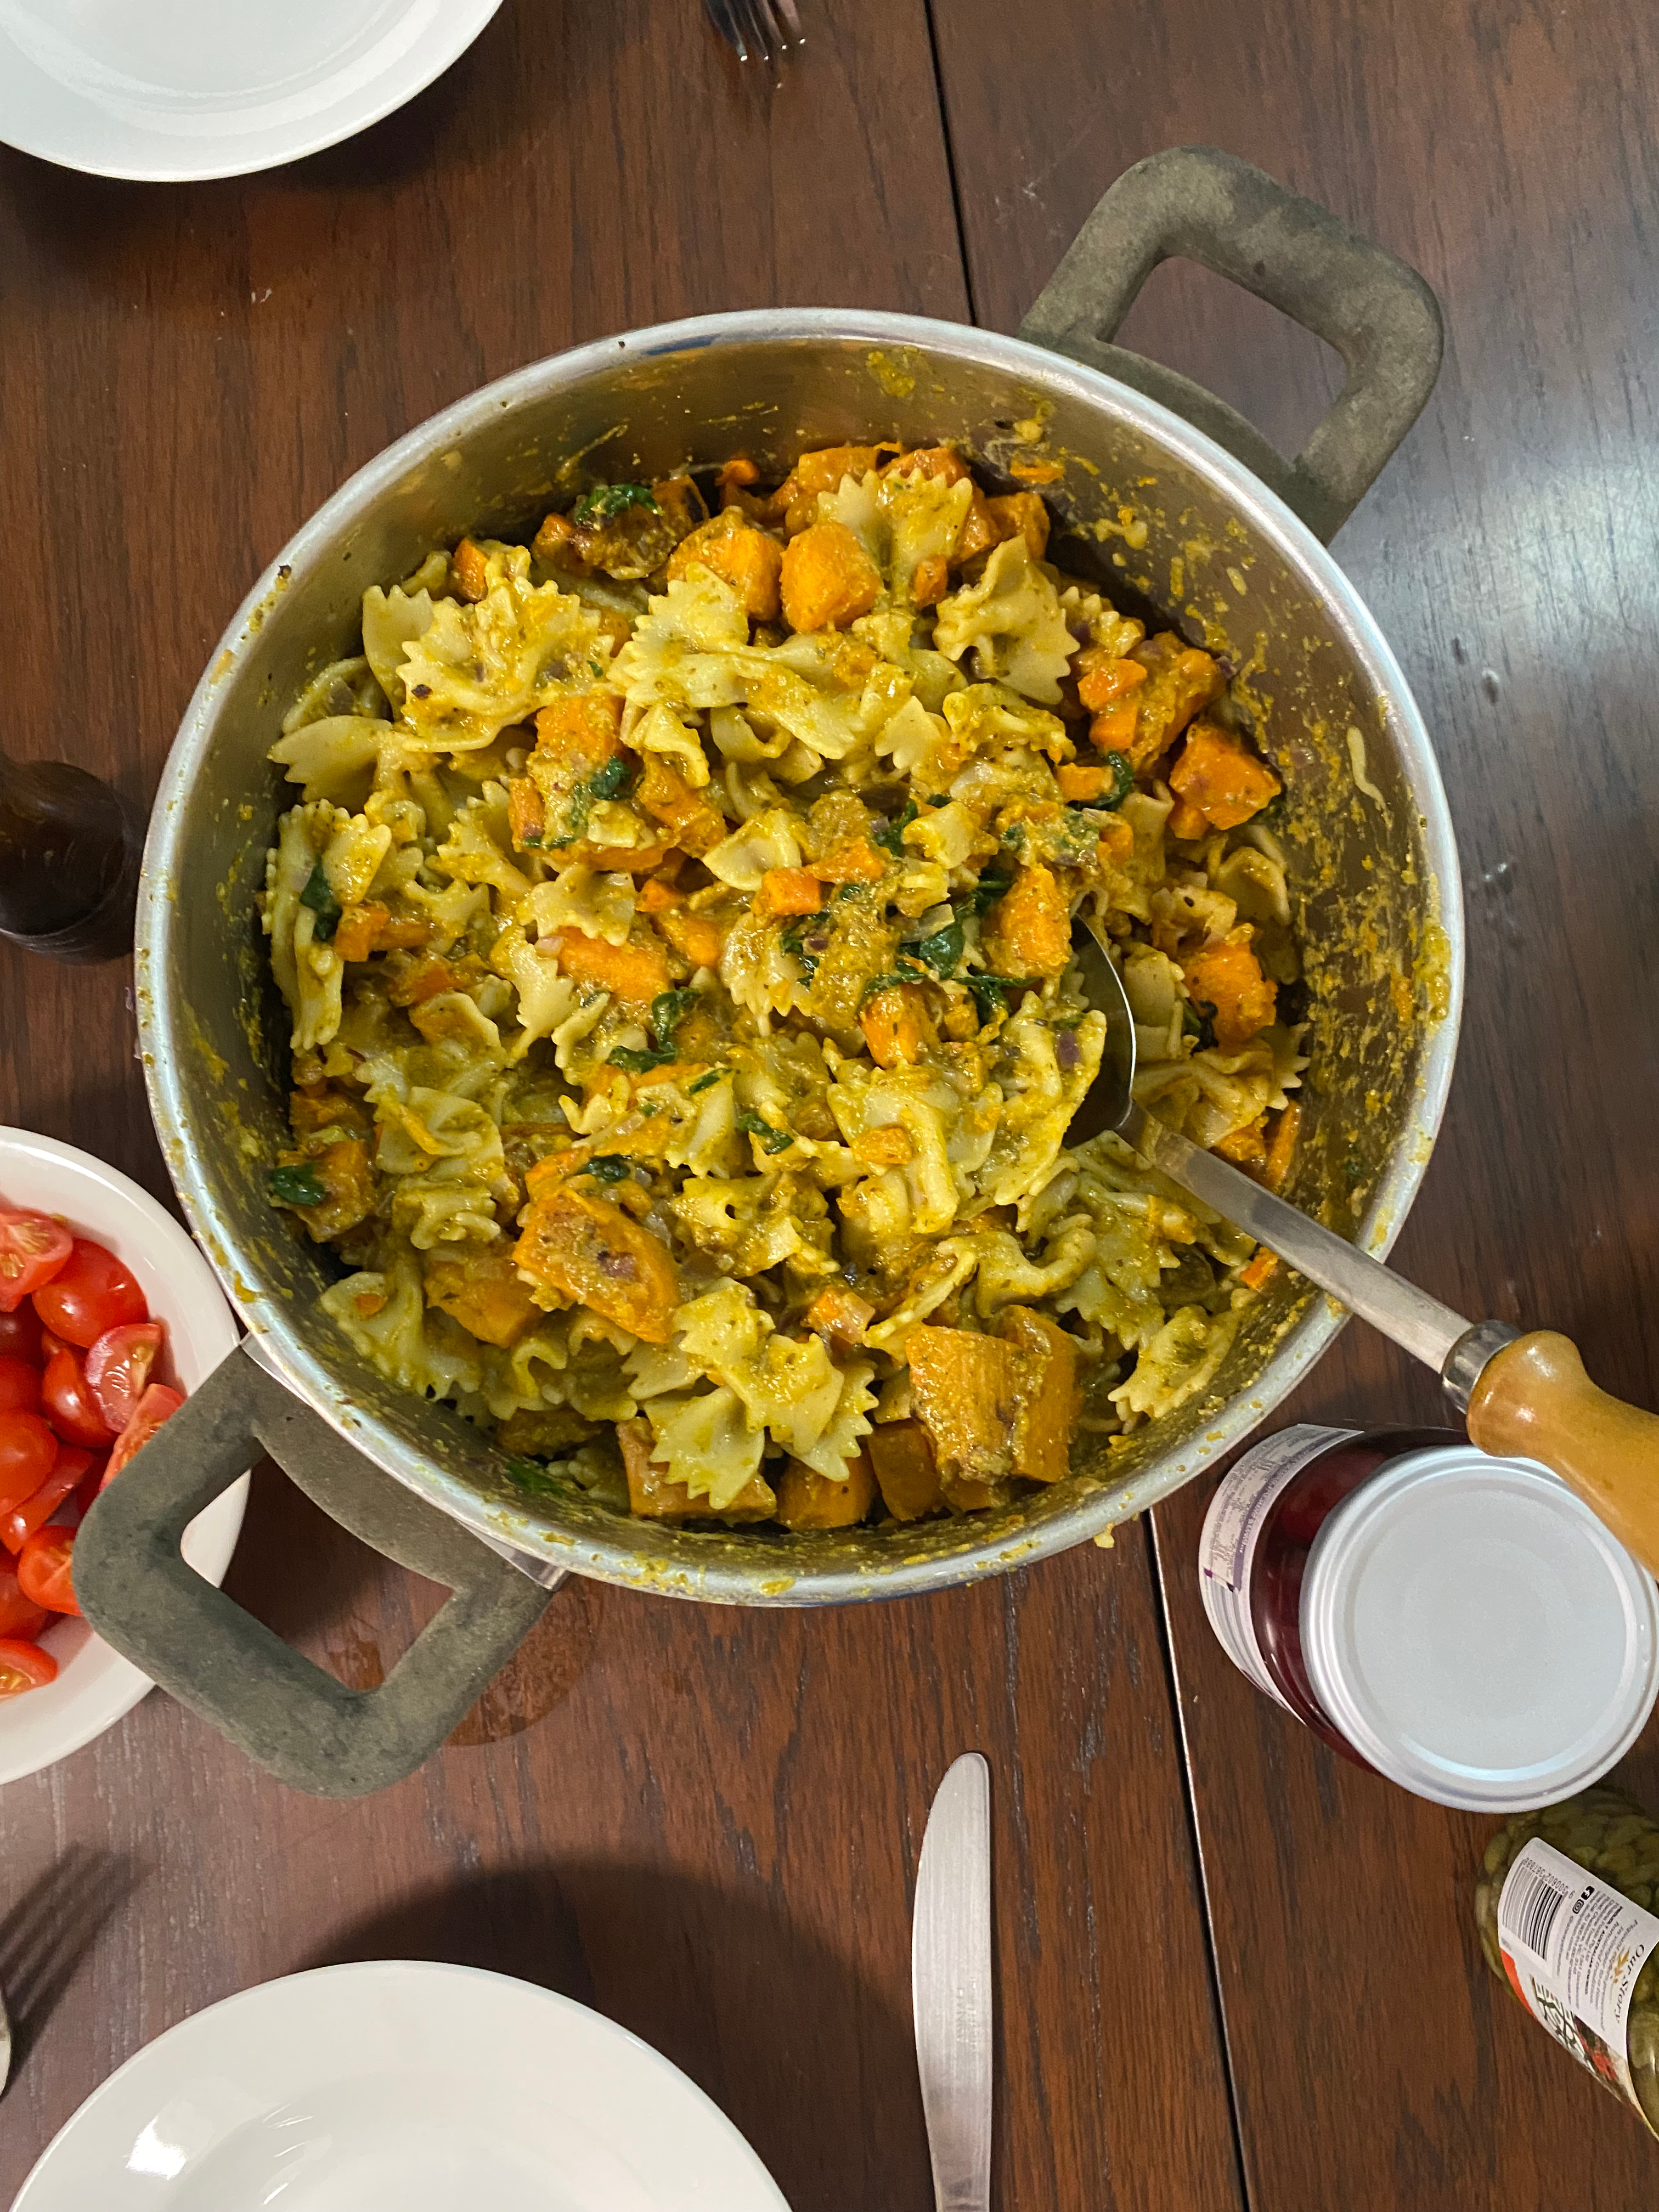
\includegraphics[keepaspectratio,width=\textwidth,height=\textheight]{Gallery/Basil Chicken Pesto}}\caption*{}\label{fig:Basil Chicken Pesto}\end{center}
\end{figure}
\newpage\begin{figure}[H]
\begin{center}\hyperref[rec:Fettuccine Alfredo]{\includegraphics[keepaspectratio,width=\textheight,height=\textwidth,angle=-90]{Gallery/Fettuccine Alfredo}}\caption*{}\label{fig:Fettuccine Alfredo}\end{center}
\end{figure}
\newpage\begin{figure}[H]
\begin{center}\hyperref[rec:Ravioli (ready meal)]{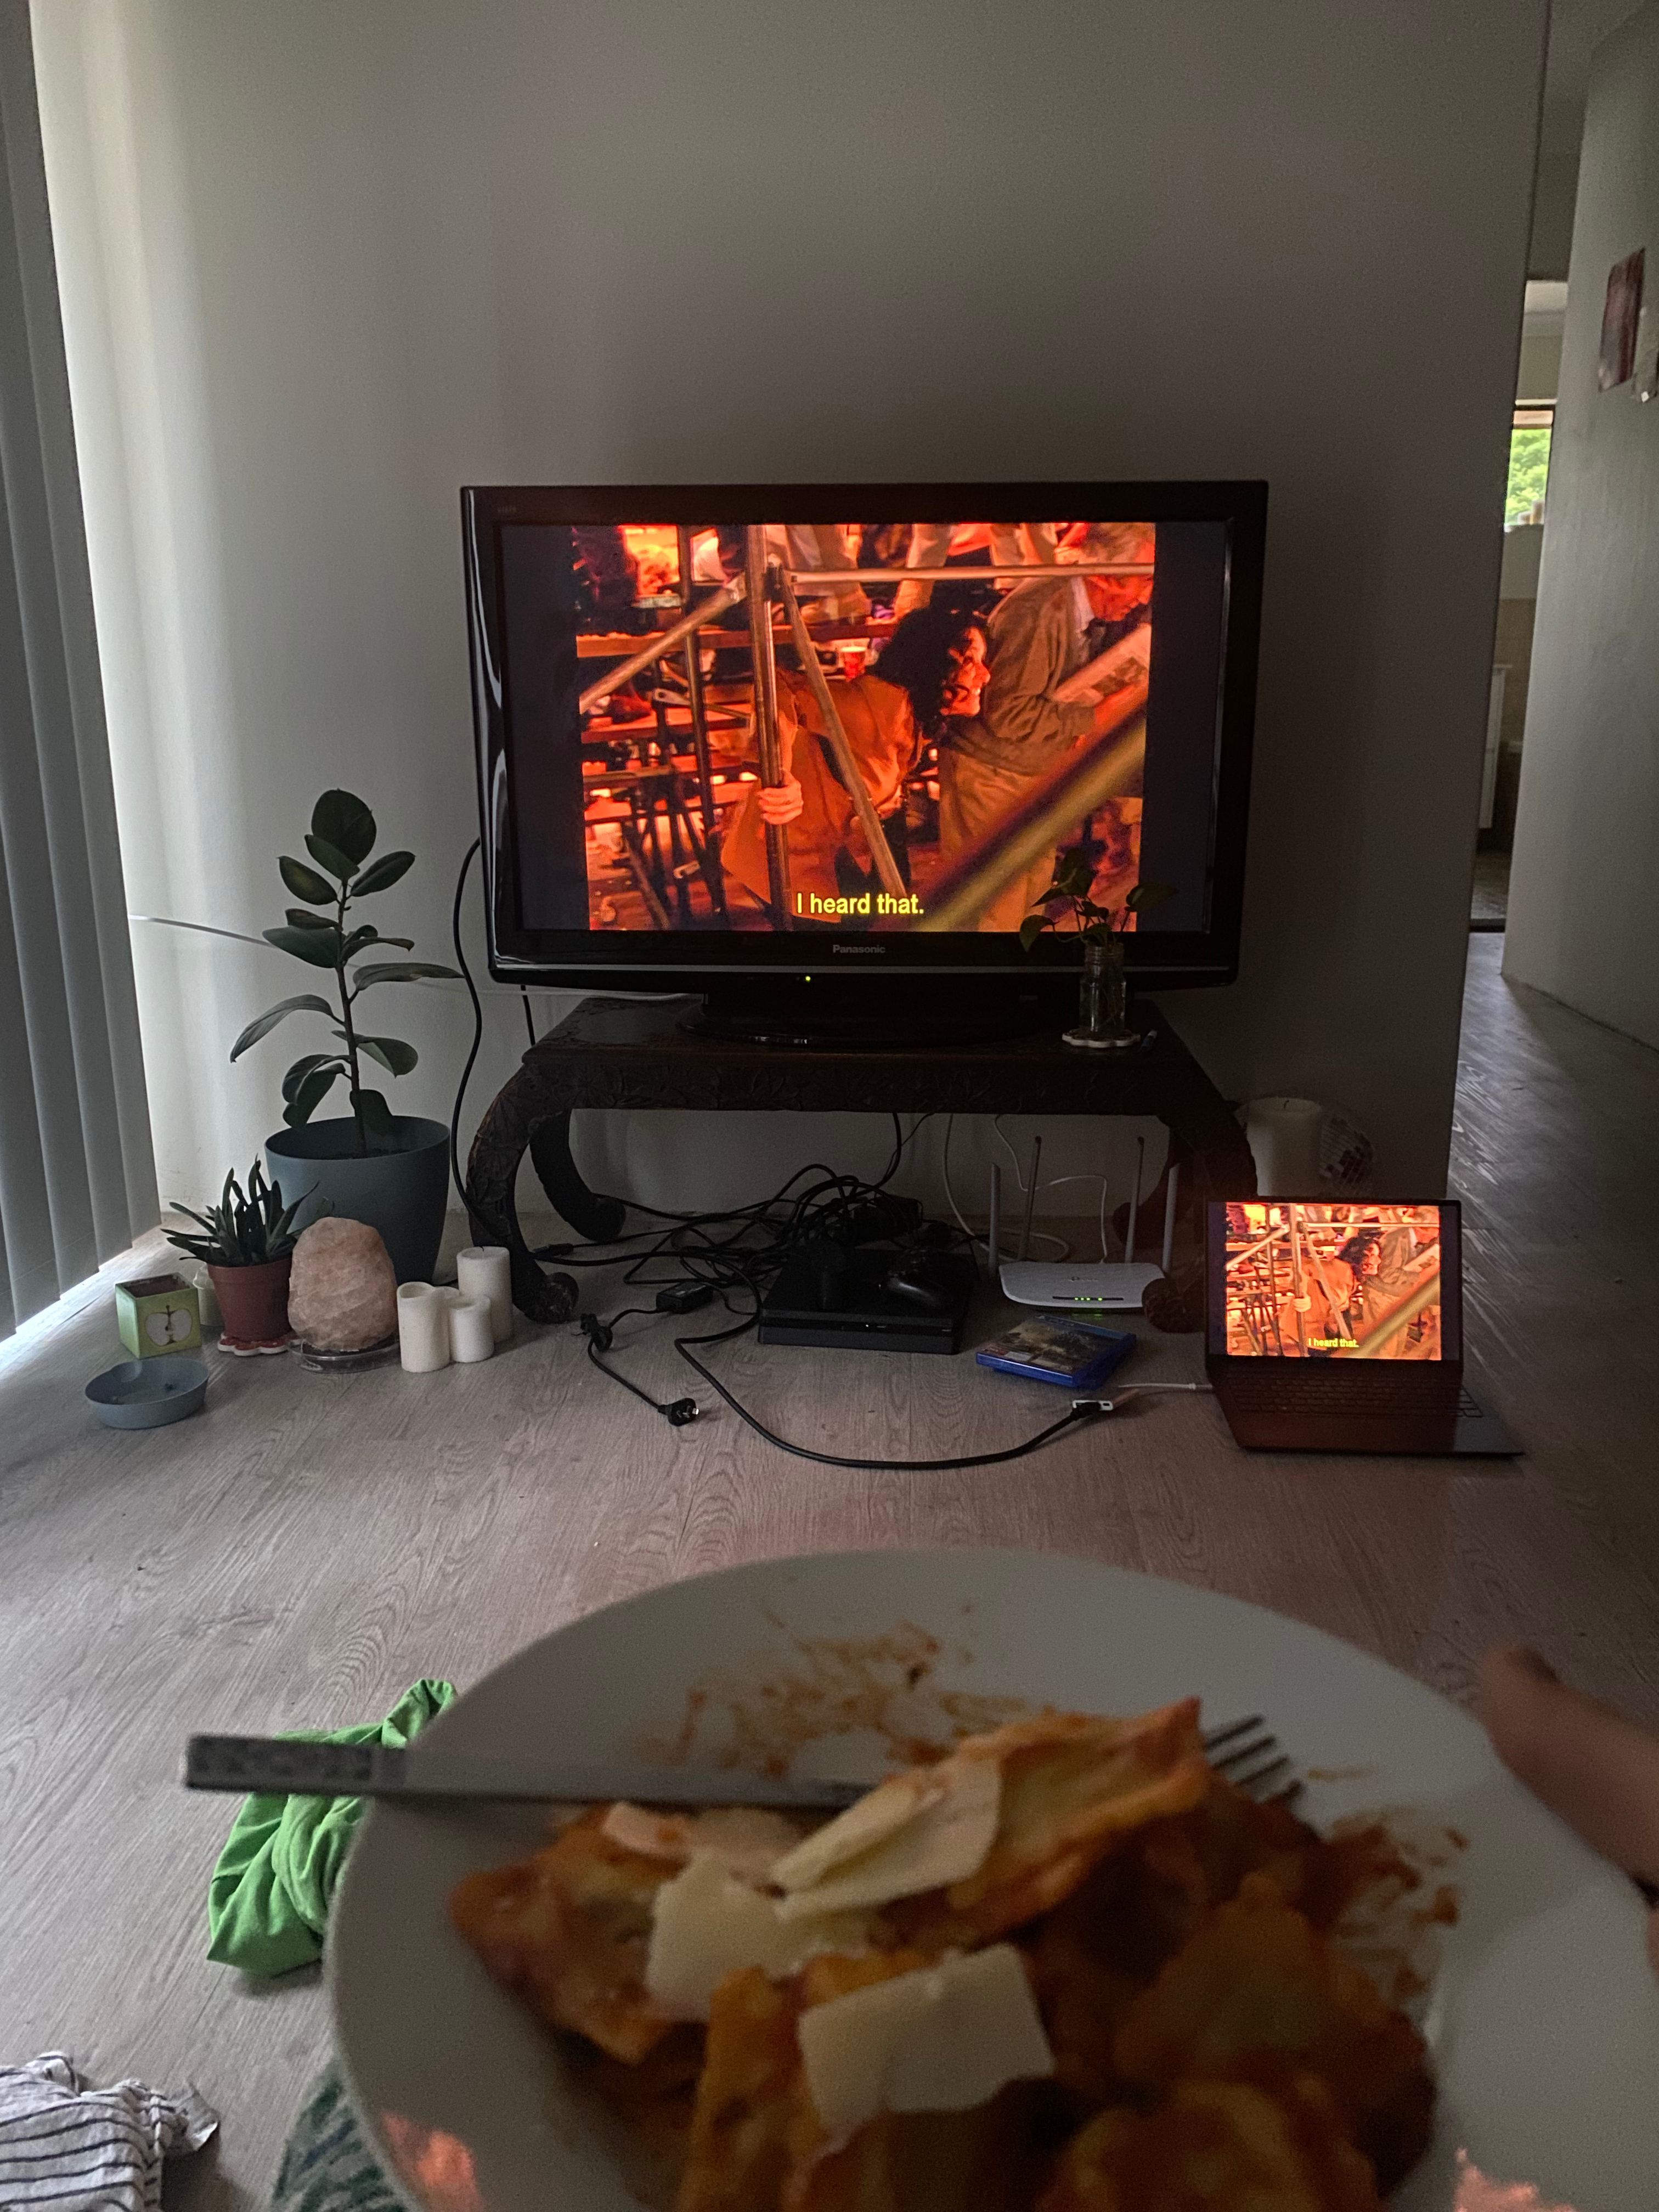
\includegraphics[keepaspectratio,width=\textwidth,height=\textheight]{Gallery/Ravioli (ready meal)}}\caption*{}\label{fig:Ravioli (ready meal)}\end{center}
\end{figure}
\newpage\begin{figure}[H]
\begin{center}\hyperref[rec:Red Sauce Rigatoni]{\includegraphics[keepaspectratio,width=\textheight,height=\textwidth,angle=-90]{Gallery/Red Sauce Rigatoni}}\caption*{}\label{fig:Red Sauce Rigatoni}\end{center}
\end{figure}
\newpage\begin{figure}[H]
\begin{center}\hyperref[rec:Bechamel Pie]{\includegraphics[keepaspectratio,width=\textheight,height=\textwidth,angle=-90]{Gallery/Bechamel Pie}}\caption*{}\label{fig:Bechamel Pie}\end{center}
\end{figure}
\newpage\begin{figure}[H]
\begin{center}\hyperref[rec:Pumpkin Quiche]{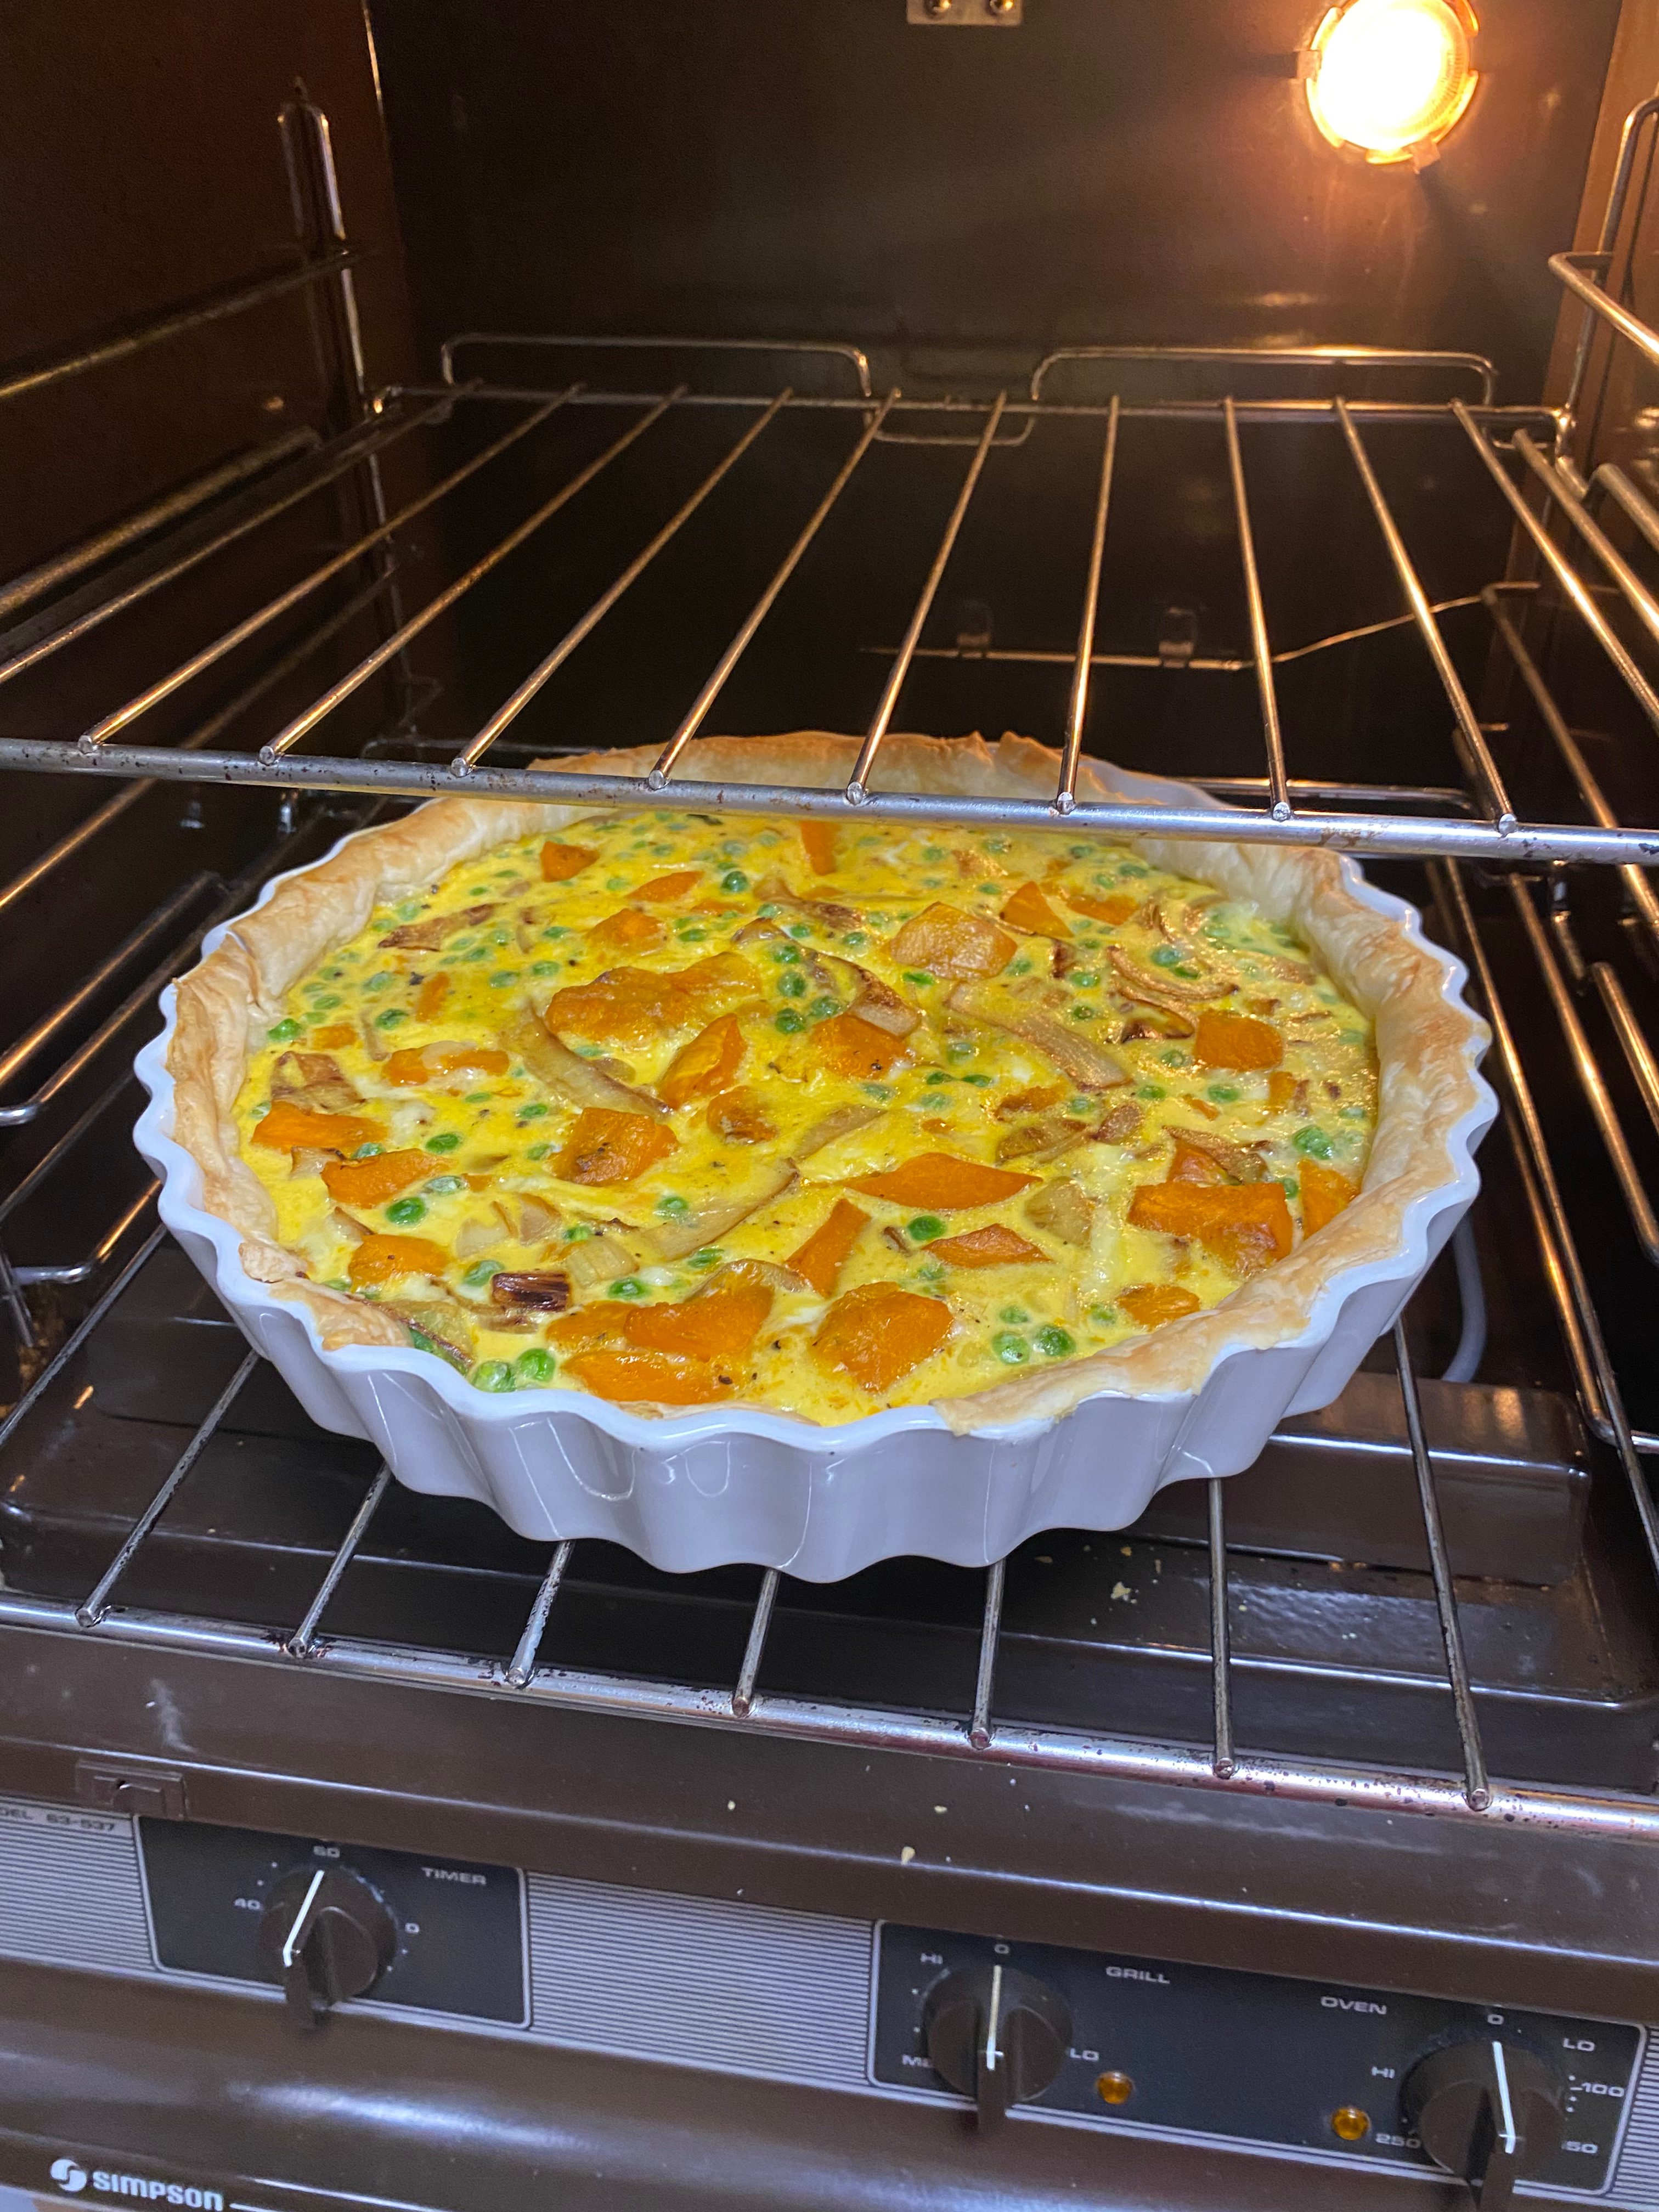
\includegraphics[keepaspectratio,width=\textwidth,height=\textheight]{Gallery/Pumpkin Quiche}}\caption*{}\label{fig:Pumpkin Quiche}\end{center}
\end{figure}
\newpage\begin{figure}[H]
\begin{center}\hyperref[rec:Tarte Dijonnaise]{\includegraphics[keepaspectratio,width=\textheight,height=\textwidth,angle=-90]{Gallery/Tarte Dijonnaise}}\caption*{}\label{fig:Tarte Dijonnaise}\end{center}
\end{figure}
\newpage\begin{figure}[H]
\begin{center}\hyperref[rec:Margherita Pizza]{\includegraphics[keepaspectratio,width=\textwidth,height=\textheight]{Gallery/Margherita Pizza}}\caption*{}\label{fig:Margherita Pizza}\end{center}
\end{figure}
\newpage\begin{figure}[H]
\begin{center}\hyperref[rec:Za'atar Munoushee]{\includegraphics[keepaspectratio,width=\textheight,height=\textwidth,angle=-90]{Gallery/Za'atar Munoushee}}\caption*{}\label{fig:Za'atar Munoushee}\end{center}
\end{figure}
\newpage\begin{figure}[H]
\begin{center}\hyperref[rec:Broccoli Paella]{\includegraphics[keepaspectratio,width=\textheight,height=\textwidth,angle=-90]{Gallery/Broccoli Paella}}\caption*{}\label{fig:Broccoli Paella}\end{center}
\end{figure}
\newpage\begin{figure}[H]
\begin{center}\hyperref[rec:Caramelised Onion and Tomato Risotto]{\includegraphics[keepaspectratio,width=\textheight,height=\textwidth,angle=-90]{Gallery/Caramelised Onion and Tomato Risotto}}\caption*{}\label{fig:Caramelised Onion and Tomato Risotto}\end{center}
\end{figure}
\newpage\begin{figure}[H]
\begin{center}\hyperref[rec:Chinese Fried Rice]{\includegraphics[keepaspectratio,width=\textheight,height=\textwidth,angle=-90]{Gallery/Chinese Fried Rice}}\caption*{}\label{fig:Chinese Fried Rice}\end{center}
\end{figure}
\newpage\begin{figure}[H]
\begin{center}\hyperref[rec:Potato Gratin]{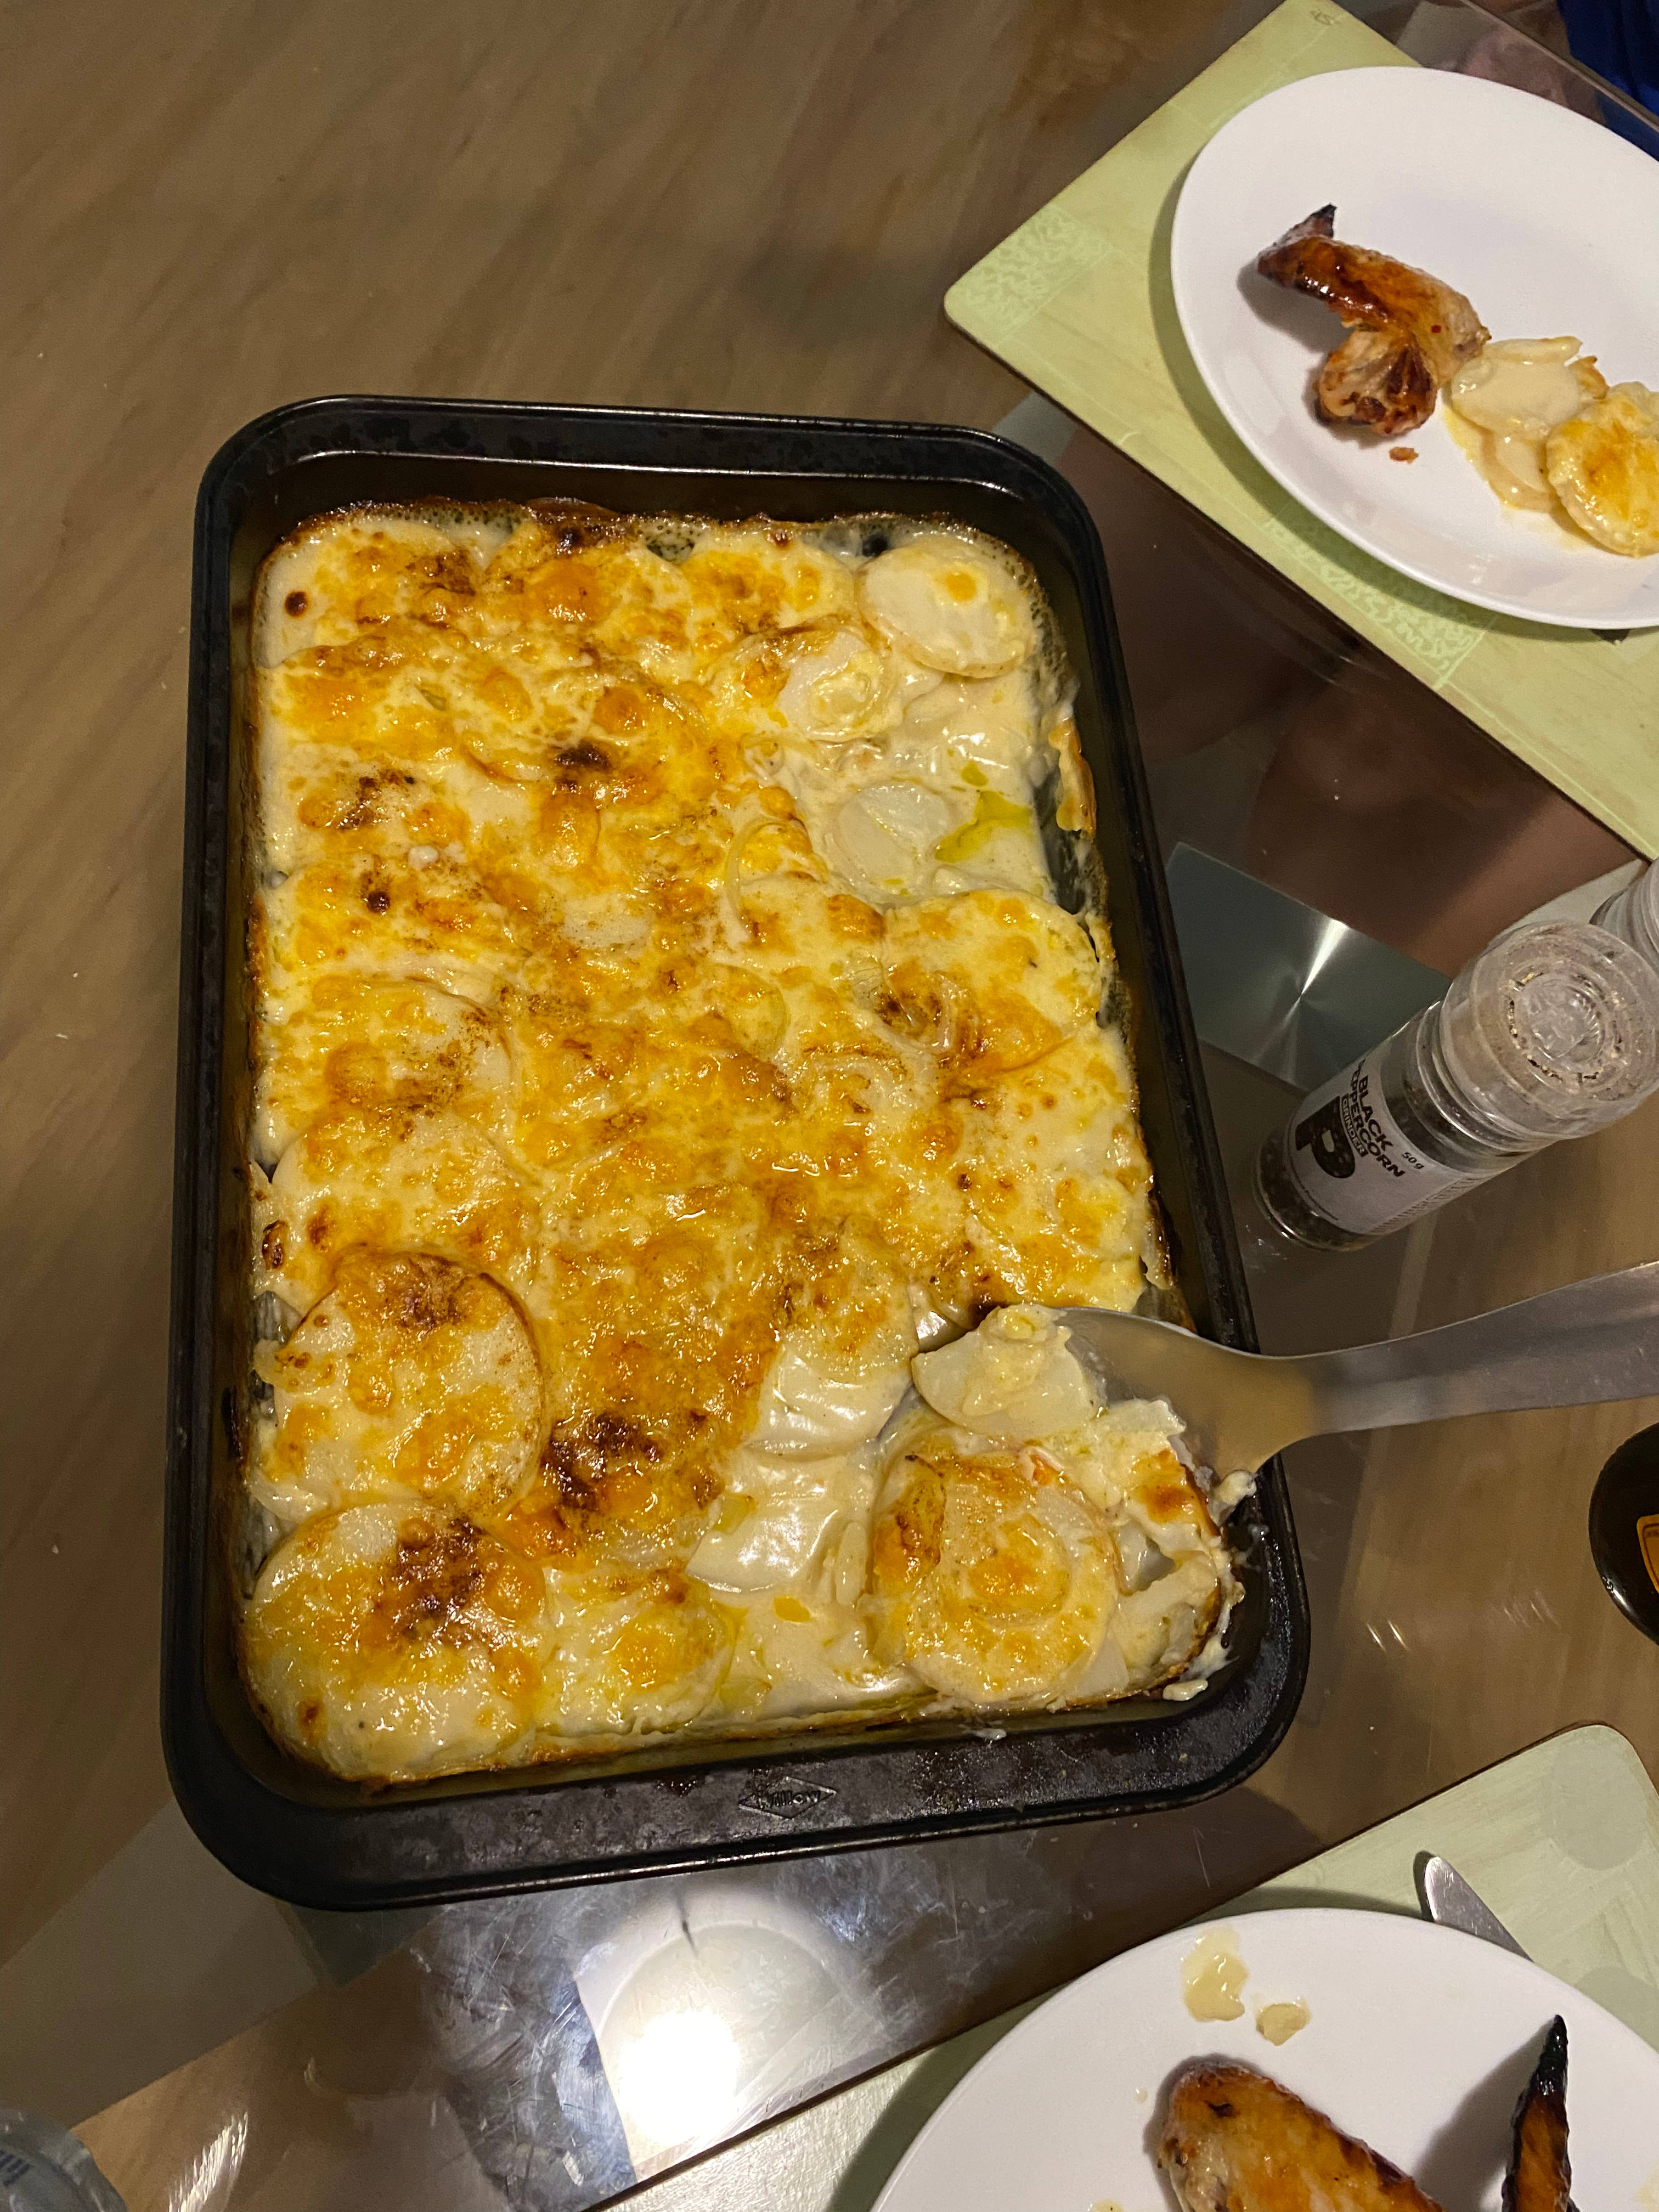
\includegraphics[keepaspectratio,width=\textwidth,height=\textheight]{Gallery/Potato Gratin}}\caption*{}\label{fig:Potato Gratin}\end{center}
\end{figure}
\newpage\begin{figure}[H]
\begin{center}\hyperref[rec:Chicken Caesar Salad]{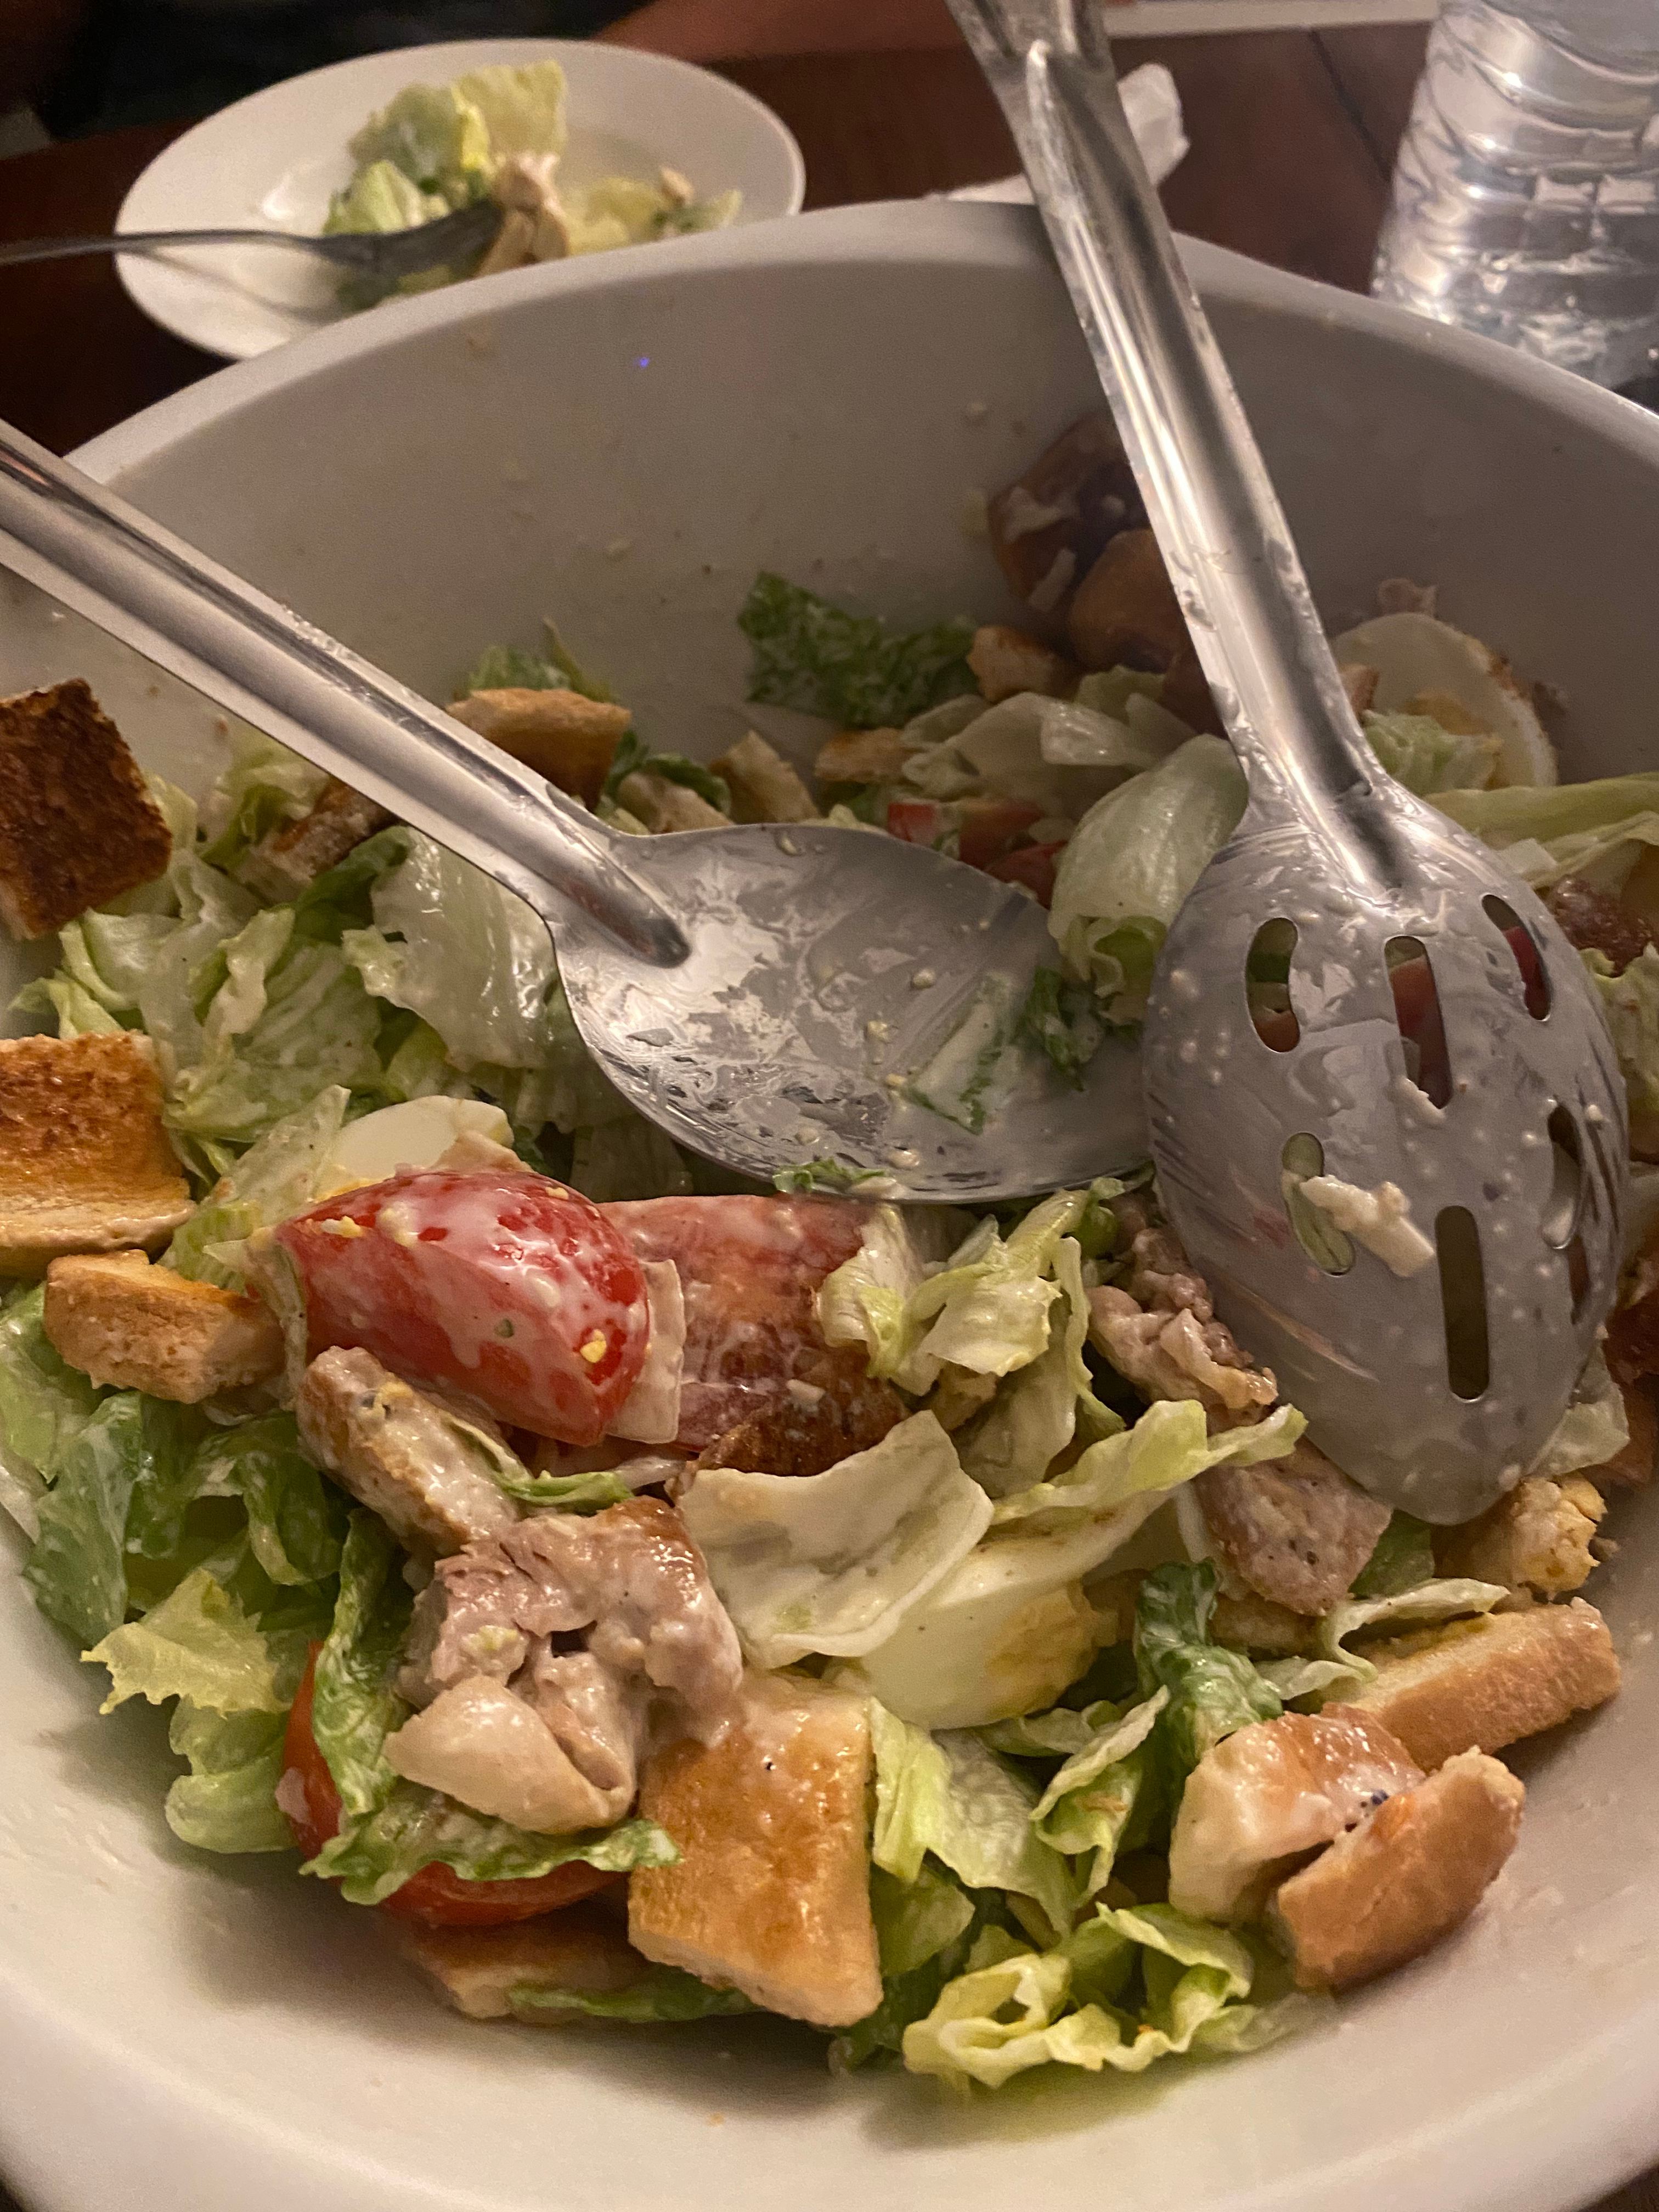
\includegraphics[keepaspectratio,width=\textwidth,height=\textheight]{Gallery/Chicken Caesar Salad}}\caption*{}\label{fig:Chicken Caesar Salad}\end{center}
\end{figure}
\newpage\begin{figure}[H]
\begin{center}\hyperref[rec:Chicken Fatteh]{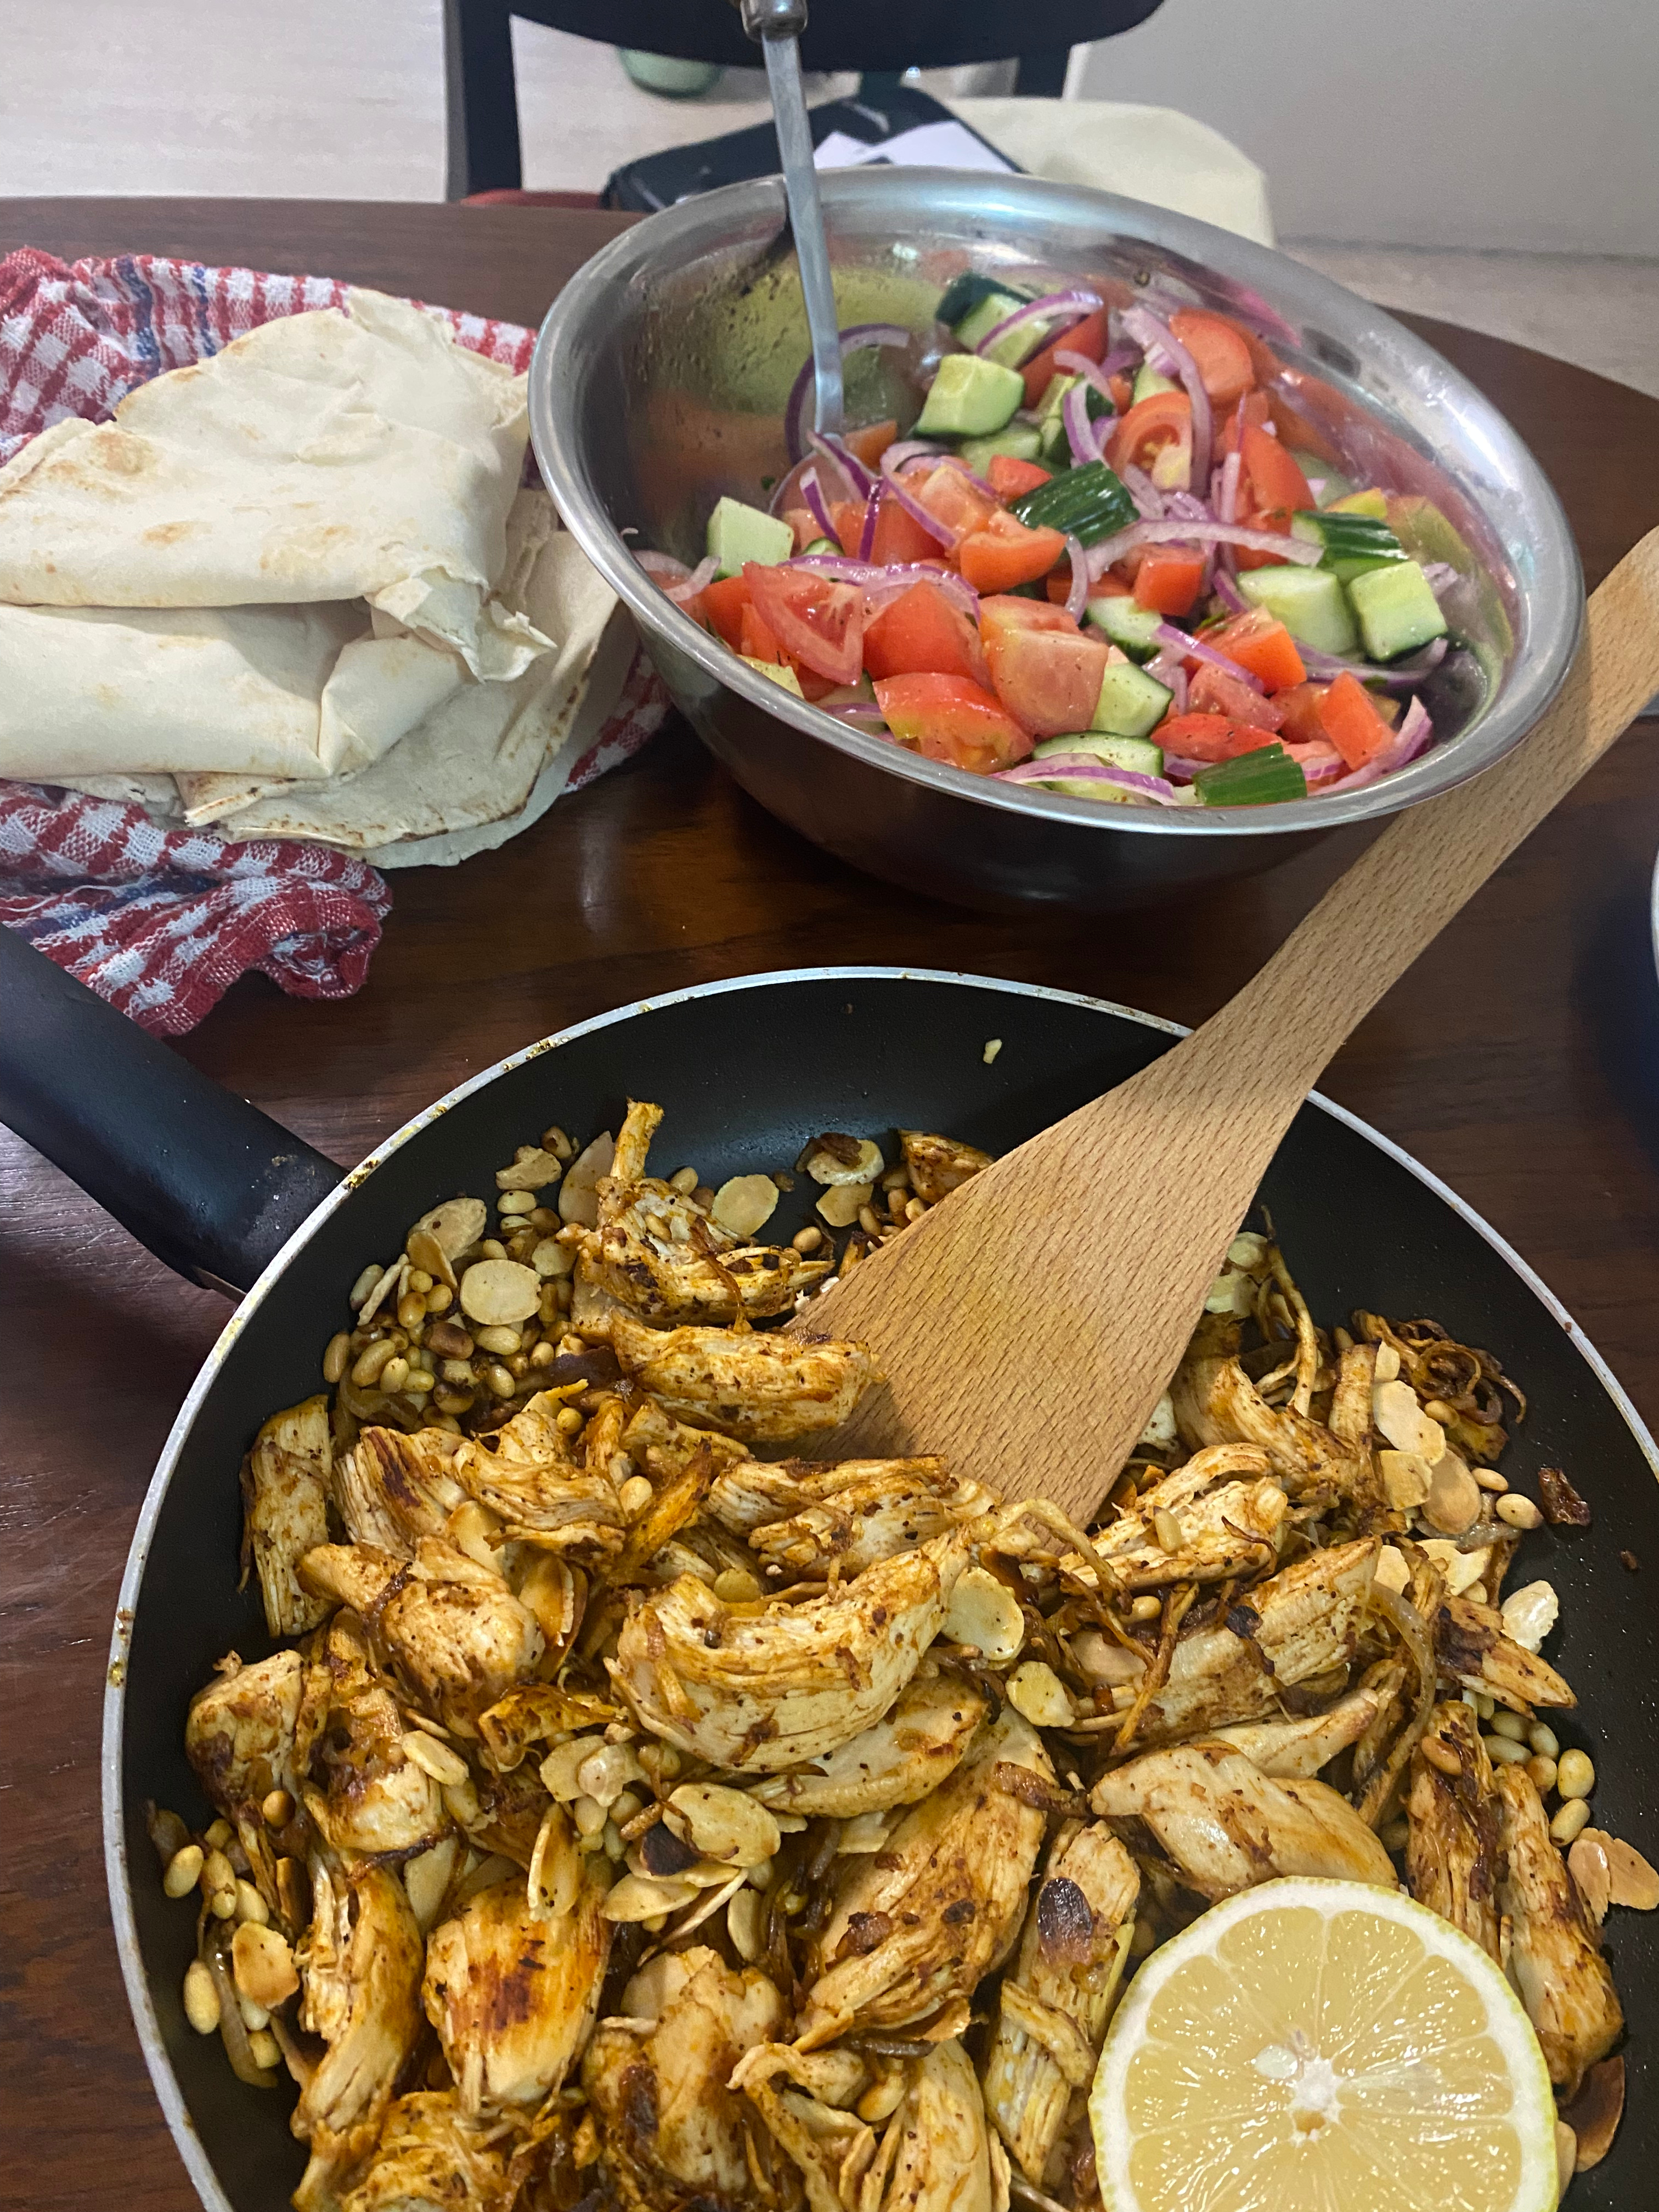
\includegraphics[keepaspectratio,width=\textwidth,height=\textheight]{Gallery/Chicken Fatteh}}\caption*{}\label{fig:Chicken Fatteh}\end{center}
\end{figure}
\newpage\begin{figure}[H]
\begin{center}\hyperref[rec:Sausages and Chips]{\includegraphics[keepaspectratio,width=\textheight,height=\textwidth,angle=-90]{Gallery/Sausages and Chips}}\caption*{}\label{fig:Sausages and Chips}\end{center}
\end{figure}
\newpage\begin{figure}[H]
\begin{center}\hyperref[rec:Egg Fried Rice]{\includegraphics[keepaspectratio,width=\textheight,height=\textwidth,angle=-90]{Gallery/Egg Fried Rice}}\caption*{}\label{fig:Egg Fried Rice}\end{center}
\end{figure}
\newpage\begin{figure}[H]
\begin{center}\hyperref[rec:Steak Tacos]{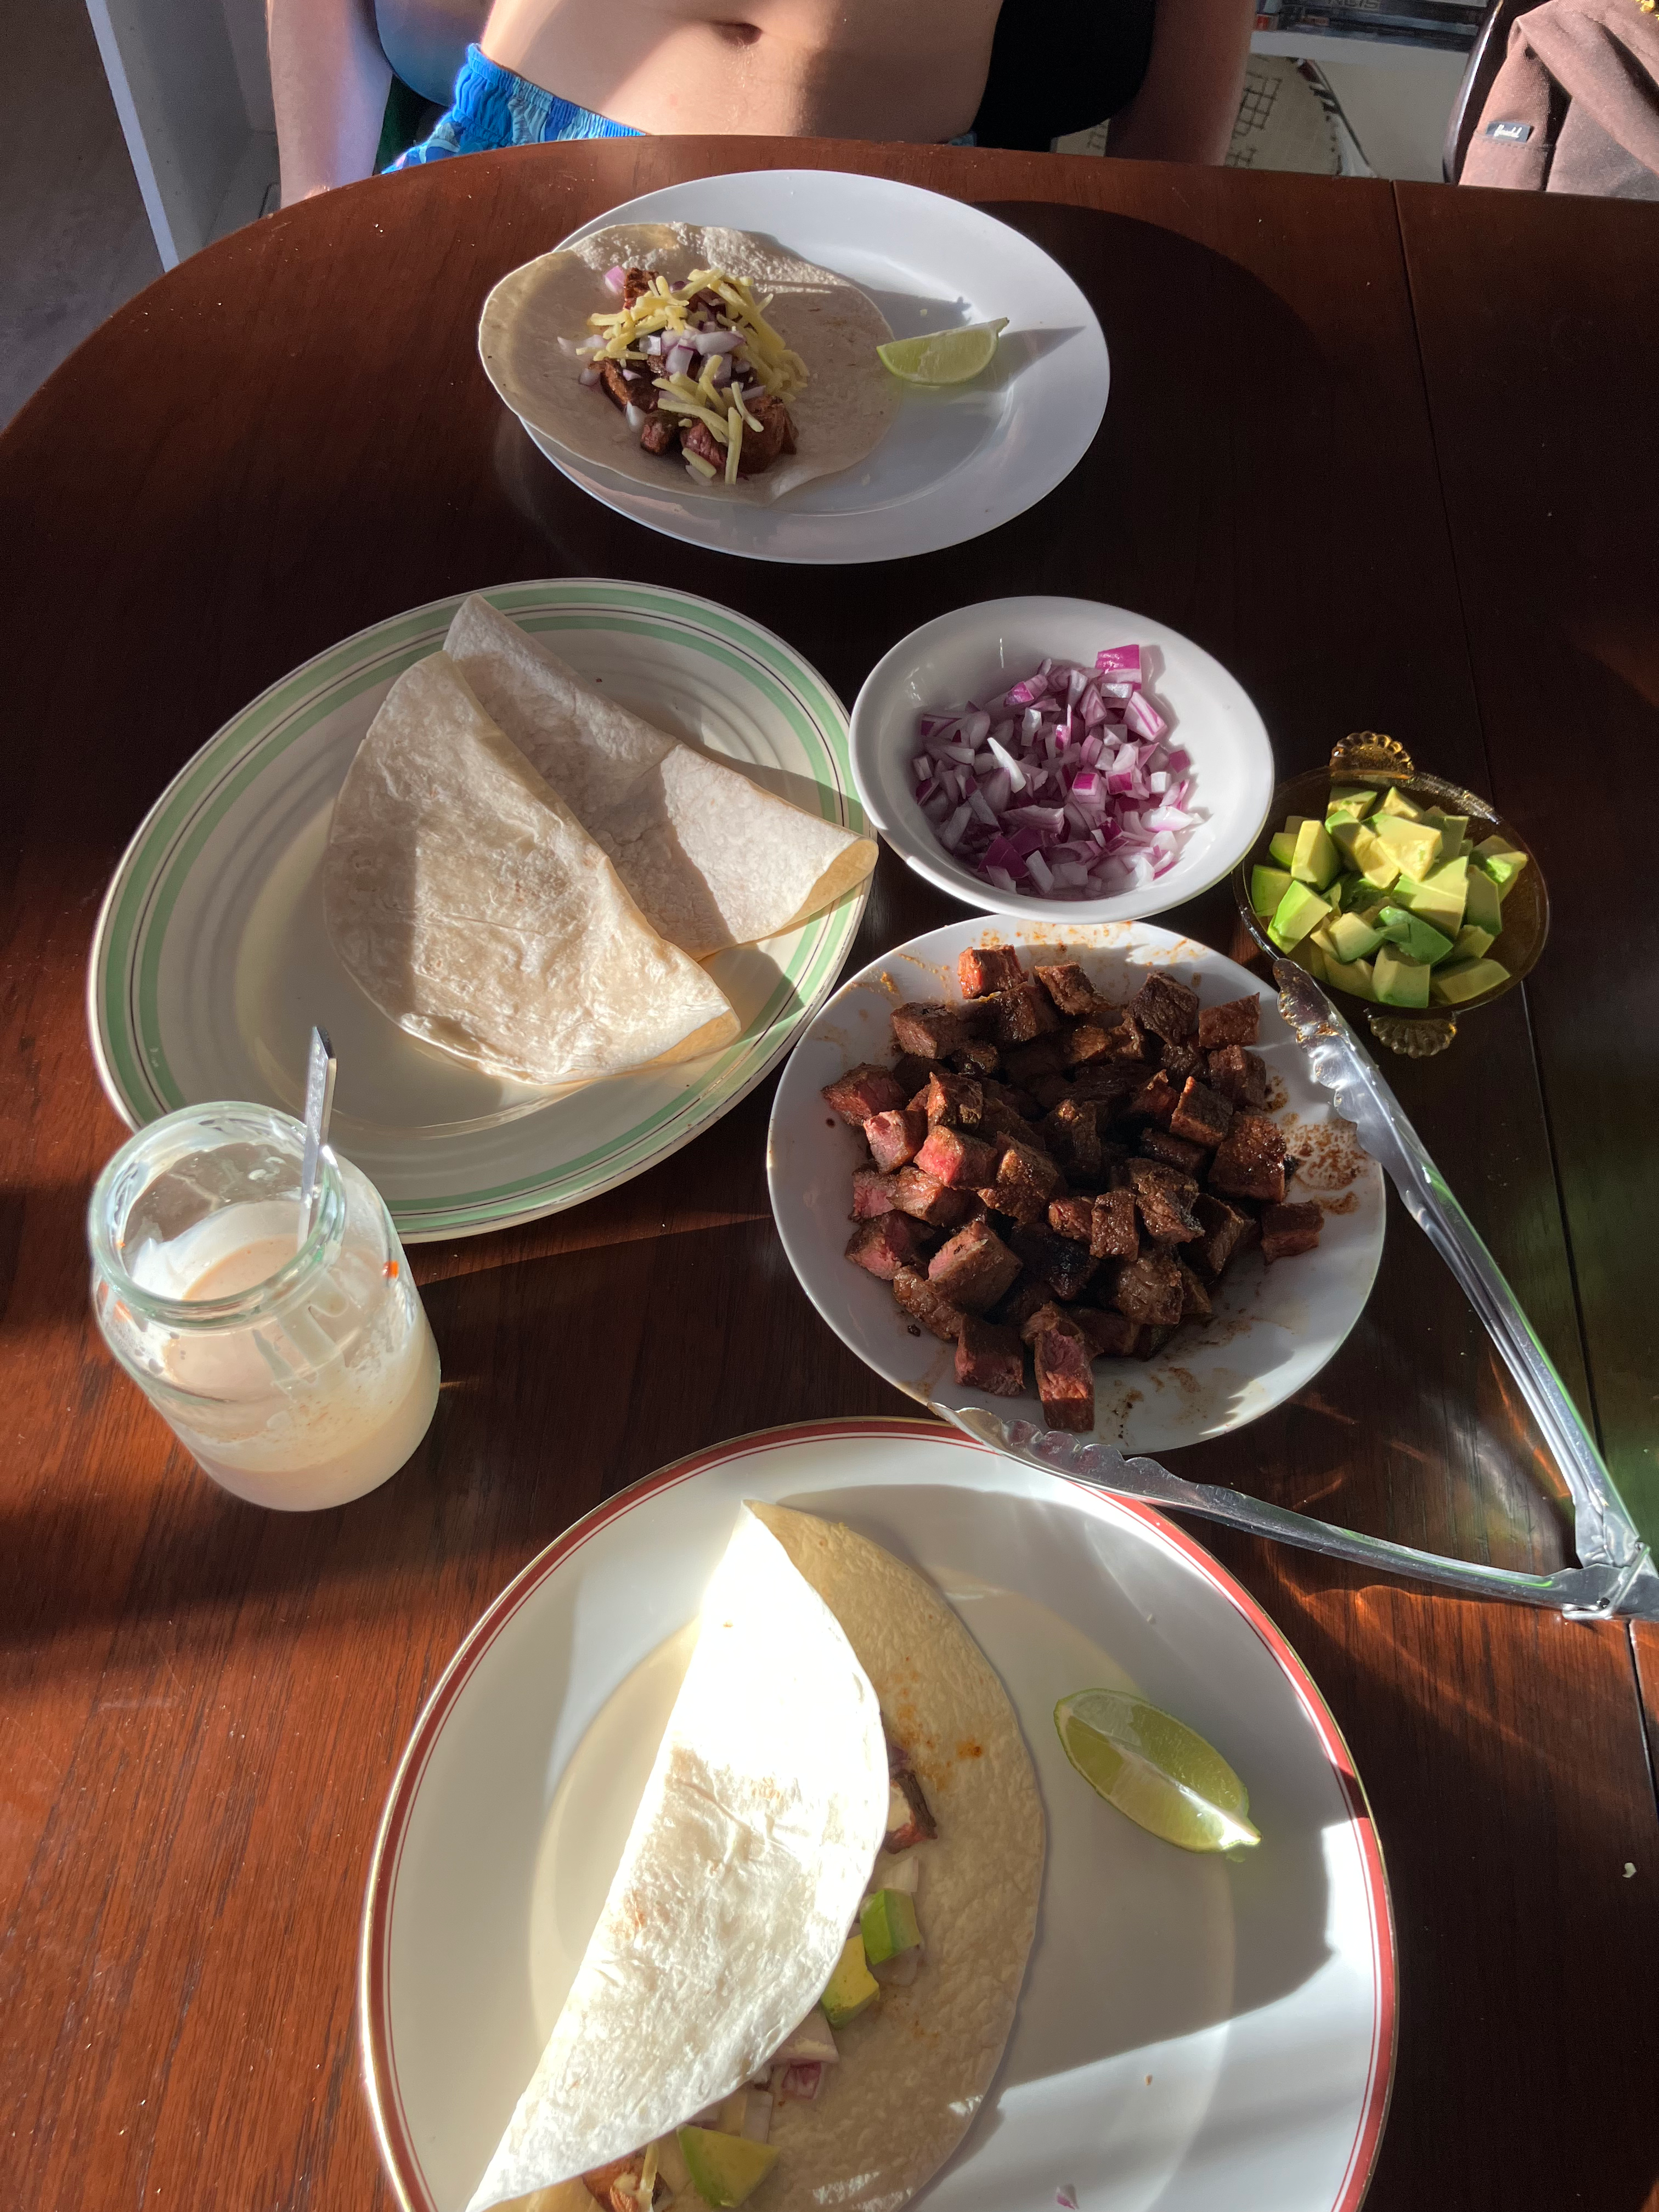
\includegraphics[keepaspectratio,width=\textwidth,height=\textheight]{Gallery/Steak Tacos}}\caption*{}\label{fig:Steak Tacos}\end{center}
\end{figure}


\newpage
\color{white}.\color{black}
\vspace{5cm}
\part{\Huge Indices}
\newpage
\printindex
\printindex[prop]
\printindex[cuisine]
\printindex[key]
\end{document}